% VERSION 3 : VERSION COURTE. main_v2 reste la version longue et de reference.
%
% CE QUE CETTE VERSION EST, ET CE QU'ELLE N'EST PAS. Kelian a demande le
% 11 septembre 2026 une reduction reelle d'environ 20 %, en ecartant explicitement
% la norme de l'Institut des actuaires (« environ 70 pages de corps, hors annexes »).
% La v3 retire donc QUATORZE SECTIONS du document, chacune remplacee par une
% section courte qui dit ce qu'elle etablissait et cite le script qui le porte.
%
% CE QUI REND CE RETRAIT ACCEPTABLE : main_v2.tex, ses chapitres et ses annexes ne
% sont PAS modifies. Les quatorze sections y figurent integralement. La v3 est une
% version courte A COTE, jamais un remplacement, et le choix entre les deux reste
% entier.
%
% LES CHAPITRES DE LA V3 SONT GENERES, PAS ECRITS. La regle du projet interdit de
% dupliquer un chapitre pour faire evoluer une version, parce que deux textes a
% maintenir divergent en une semaine. Les sept chapitres restructures sont donc
% DERIVES des chapitres partages par exploratory/memoire_cascade/construire_v3.py.
% Corriger un chapitre de la v3 se fait dans chapitres/, puis par relance du
% script. Ne jamais editer chapitres_v3/ a la main.
%
% Les douze autres pieces sont appelees TELLES QUELLES depuis chapitres/, donc
% sans copie et sans risque de divergence.

\documentclass[11pt,a4paper]{report}

% Meme preambule que la v2 : police Palatino, sans couleur, encadres en filets.
% La v3 ne change pas le style, elle change la longueur.
% Préambule V2 : STYLE CLASSIQUE DE MONOGRAPHIE. Appelé par main_v2.tex.
%
% CE FICHIER NE CHANGE QUE L'APPARENCE. Les chapitres sont EXACTEMENT les mêmes
% fichiers que ceux de main.tex : aucun mot, aucun nombre, aucune structure ne
% diffère entre les deux versions. C'est la condition pour que la comparaison
% porte sur le style seul, et c'est aussi ce qui évite de maintenir deux textes.
%
% CE QUI CHANGE, ET POURQUOI
%   1. POLICE. Palatino (mathpazo) au lieu de Latin Modern. C'est une romaine de
%      la Renaissance revisitée : c'est elle qui donne l'aspect << texte ancien >>.
%      Sa hauteur d'x est grande, donc l'interligne est ouvert à 1,05, sans quoi
%      le gris de la page devient trop dense.
%   2. AUCUNE COULEUR. Tous les noms de couleurs du projet sont redéfinis en NOIR,
%      ce qui neutralise les \textcolor{navy} des chapitres sans les éditer. Les
%      liens restent cliquables mais s'impriment en noir.
%   3. LES ENCADRÉS DEVIENNENT DES FILETS. Les 66 blocs << clé >> et les 48 blocs
%      << attention >> perdent leur fond bleu et leur cadre arrondi. Ils gardent
%      leur distinction, mais par la TYPOGRAPHIE et non par la couleur : filets
%      haut et bas pour la synthèse, filet vertical épais pour l'avertissement.
%      C'est le dispositif des monographies imprimées, et il survit à la
%      photocopie comme à l'impression en noir et blanc.
%   4. TITRES. Petites capitales et filets, jamais de gras coloré. Les têtes de
%      paragraphe passent en italique : elles sont ici des phrases entières, et
%      une phrase entière en gras alourdit la page.
%   5. TITRES COURANTS. Chapitre en petites capitales en tête de page. Signal
%      classique, et utile sur un document de cette longueur.
%
% CE QUI NE CHANGE PAS, ET C'EST DÉLIBÉRÉ
%   LA GÉOMÉTRIE. Les marges restent à 2,4 cm. Une monographie classique aurait
%   une justification plus étroite, mais la lisibilité des cinquante figures est
%   calibrée sur CETTE largeur : \figover déborde à 1,14 fois la justification et
%   \figcle remplit la page. Rétrécir le bloc de texte rendrait les étiquettes
%   illisibles, ce qui est le défaut que la note de \figover documente. Le style
%   ne se paie pas en lisibilité des résultats.
%
%   LES CHIFFRES RESTENT ALIGNÉS (pas de chiffres elzéviriens). Palatino en
%   propose, et ils sont plus élégants dans un texte courant. Ils sont refusés
%   ici : ce document se lit pour ses nombres, et des chiffres de hauteur
%   inégale se comparent mal dans une colonne de tableau.

\usepackage[utf8]{inputenc}
\usepackage[T1]{fontenc}
\usepackage[sc]{mathpazo}          % Palatino, avec vraies petites capitales
\linespread{1.05}                  % obligatoire avec Palatino : grande hauteur d'x
\usepackage[french]{babel}
\usepackage[margin=2.4cm]{geometry}
\usepackage{microtype}

% Palatino est PLUS LARGE que Latin Modern a taille nominale egale, si bien que
% des paragraphes qui tenaient debordent. On autorise donc TeX a etirer les
% blancs entre mots en dernier recours, ce qui resorbe les debordements de
% PARAGRAPHE sans toucher une ligne des chapitres. Les debordements de TABLEAU,
% eux, ne s'y reduisent pas : une colonne trop large reste trop large, et cela
% se corrige dans le tableau ou pas du tout.
\setlength{\emergencystretch}{2.5em}
\usepackage{booktabs}
\usepackage{array}
\usepackage[table]{xcolor}
\usepackage{amsmath}
\usepackage{amssymb}
\usepackage{mathtools}
\usepackage{enumitem}
\usepackage[most]{tcolorbox}
\usepackage{tabularx}
\usepackage{longtable}
\usepackage{graphicx}
\usepackage{eurosym}
\usepackage{caption}
\usepackage{titlesec}
\usepackage{fancyhdr}
\usepackage{amsthm}
\usepackage[round,authoryear]{natbib}
\usepackage{hyperref}

% ---------------------------------------------------------------------------
% FIGURES : dispositif IDENTIQUE à la version 1, et il ne doit pas bouger.
% Voir la note du préambule de la version 1 pour le motif complet.
% ---------------------------------------------------------------------------
\newcommand{\figover}[1]{%
  \makebox[\textwidth][c]{\includegraphics[width=1.14\textwidth]{#1}}}

\newcommand{\figcle}[3]{%
  \begin{figure}[p]
    \centering
    \makebox[\textwidth][c]{%
      \includegraphics[width=1.10\textwidth,height=0.88\textheight,keepaspectratio]{#1}}
    \caption{#2}
    \label{#3}
  \end{figure}}

\graphicspath{{../vasicek_lab/figures/}{../cascade_qualitative/figures/}{../../outputs/}}

% ---------------------------------------------------------------------------
% ÉNONCÉS. Style classique : corps en italique pour les théorèmes, en romain
% pour les définitions, ce qui les distingue sans numérotation séparée.
% ---------------------------------------------------------------------------
\theoremstyle{plain}
\newtheorem{theorem}{Théorème}[chapter]
\newtheorem{proposition}[theorem]{Proposition}
\newtheorem{lemma}[theorem]{Lemme}
\theoremstyle{definition}
\newtheorem{definition}[theorem]{Définition}

\newcommand{\R}{\mathbb{R}}
\newcommand{\E}{\mathbb{E}}
\newcommand{\Prob}{\mathbb{P}}
\newcommand{\Var}{\mathrm{Var}}
% VaR et TVaR sont RESERVEES a la charge annuelle agregee L, c'est-a-dire a la mesure de
% capital. Le quantile de la severite d'un SINISTRE UNIQUE est un autre objet : il porte le
% symbole q, et sa moyenne de queue le symbole q barre. Ne pas les confondre : un niveau de
% 99,5 % n'a de sens reglementaire que sur un horizon ANNUEL, et une perte unique n'en porte
% aucun. Voir la table des notations et le chapitre socle.
\newcommand{\VaR}{\mathrm{VaR}}
\newcommand{\TVaR}{\mathrm{TVaR}}
\newcommand{\qsev}{\mathrm{q}}
\newcommand{\qbarsev}{\overline{\mathrm{q}}}
\newcommand{\dd}{\mathrm{d}}
\newcommand{\indic}{\mathbf{1}}
\providecommand{\up}[1]{\textsuperscript{#1}}

% ---------------------------------------------------------------------------
% PALETTE : tous les noms de la version 1 existent encore, et ils valent NOIR.
% C'est ce qui rend les chapitres réutilisables sans une seule édition : les
% cinq \textcolor{navy} de la table des notations s'impriment en noir, et les
% cellules colorées des tables de synthèse deviennent blanches.
% ---------------------------------------------------------------------------
\definecolor{navy}{gray}{0}
\definecolor{bluemid}{gray}{0}
\definecolor{lightblue}{gray}{1}
\definecolor{accent}{gray}{0}
\definecolor{green}{gray}{0}
\definecolor{lightgreen}{gray}{1}
\definecolor{softgreen}{gray}{1}
\definecolor{softamber}{gray}{1}

\hypersetup{colorlinks=true, linkcolor=black, urlcolor=black, citecolor=black,
  pdftitle={Quantification du SCR lie a la non-conformite DORA par la cascade dirigee},
  pdfauthor={Kelian Kaddouri}}

% ---------------------------------------------------------------------------
% LES DEUX ENCADRÉS, EN TYPOGRAPHIE PLUTÔT QU'EN COULEUR.
% Ils restent des environnements tcolorbox pour une raison pratique : ils
% doivent pouvoir se COUPER entre deux pages, ce qu'un simple \hrule autour
% d'un bloc ne sait pas faire proprement sur des blocs de dix lignes.
%   cle       : filets haut et bas, pleine justification. C'est le << résumé
%               encadré >> des monographies : il arrête l'oeil sans le colorer.
%   attention : filet vertical épais et retrait. Distinction lisible en noir et
%               blanc, et hiérarchie claire, l'avertissement étant en retrait
%               du fil du texte quand la synthèse l'interrompt.
% ---------------------------------------------------------------------------
% NOTE DE MISE EN OEUVRE, ET ELLE A COUTE UN ESSAI. Mettre boxrule a 0pt puis
% ne relever que toprule et bottomrule NE SUFFIT PAS : le squelette << enhanced >>
% trace quand meme un filet de cheveu sur les quatre cotes, et les deux encadres
% se retrouvent tous deux cadres, donc indistinguables. L'idiome correct est
% << frame hidden >> pour supprimer le cadre, puis des << borderline >> pour ne
% dessiner que les filets voulus. Verifie sur le PDF rendu, pas sur la source.
\newtcolorbox{cle}[1][]{%
  enhanced, breakable, sharp corners,
  colback=white, frame hidden,
  borderline north={0.9pt}{0pt}{black},
  borderline south={0.9pt}{0pt}{black},
  left=0pt, right=0pt, top=8pt, bottom=8pt,
  before skip=12pt, after skip=12pt, #1}

\newtcolorbox{attention}[1][]{%
  enhanced, breakable, sharp corners,
  colback=white, frame hidden,
  borderline west={1.8pt}{0pt}{black},
  left=12pt, right=0pt, top=4pt, bottom=4pt,
  before skip=12pt, after skip=12pt, #1}

\newtcolorbox{migration}[1][]{%
  enhanced, breakable, sharp corners, colback=white, colframe=black,
  boxrule=0.4pt, left=8pt, right=8pt, top=5pt, bottom=5pt,
  before skip=8pt, after skip=8pt, #1}
\newcommand{\areprendre}[1]{\begin{migration}\footnotesize\textit{[À migrer]}~#1\end{migration}}

% ---------------------------------------------------------------------------
% VERDICTS DES TABLES DE SYNTHÈSE. La version 1 les distingue par la couleur du
% fond de cellule. Ici c'est le mot qui porte, en petites capitales : les trois
% verdicts se lisent aussi bien, et la table survit à une impression en noir.
% \cascell devient neutre : la ligne qu'elle marquait porte déjà son gras.
% ---------------------------------------------------------------------------
\newcommand{\rob}{\textsc{robuste}}
\newcommand{\feat}{\textsc{voulu}}
\newcommand{\ass}{\textsc{assumé}}
\newcommand{\oui}{$\checkmark$}
\newcommand{\non}{$\times$}
\newcommand{\cascell}{}

% ---------------------------------------------------------------------------
% TITRES. Petites capitales et filets. Aucun gras coloré.
% L'espacement resserré de la version 1 est CONSERVÉ : il économise environ un
% quart de page par chapitre, et le style n'a pas de raison de le rendre.
% ---------------------------------------------------------------------------
\titleformat{\part}[display]
  {\normalfont\filcenter}
  {\large\scshape\partname~\thepart}
  {16pt}
  {\Huge\scshape}
\titleformat{\chapter}[display]
  {\normalfont}
  {\normalsize\scshape\chaptertitlename~\thechapter}
  {8pt}
  {\huge}
  [{\vspace{6pt}\titlerule[0.8pt]}]
\titlespacing*{\chapter}{0pt}{-10pt}{22pt}
\titleformat{\section}{\normalfont\large\bfseries}{\thesection}{0.6em}{}
\titleformat{\subsection}{\normalfont\normalsize\itshape}{\thesubsection}{0.5em}{}
\titleformat{\paragraph}[runin]{\normalfont\normalsize\itshape}{}{0pt}{}
\titlespacing*{\paragraph}{0pt}{9pt}{0.55em}

\captionsetup{font=small,labelfont=sc,labelsep=period,skip=6pt}

% Titres courants : chapitre en petites capitales, filet fin, folio à droite.
\pagestyle{fancy}
\fancyhf{}
\fancyhead[L]{\small\scshape\nouppercase{\leftmark}}
\fancyhead[R]{\small\thepage}
\renewcommand{\headrulewidth}{0.4pt}
\fancypagestyle{plain}{\fancyhf{}\fancyfoot[C]{\small\thepage}%
  \renewcommand{\headrulewidth}{0pt}}

% ---------------------------------------------------------------------------
% PAGE DE TITRE classique : filets, petites capitales, pas de couleur.
% ---------------------------------------------------------------------------
\title{%
  \vspace{-0.8cm}
  \rule{\textwidth}{1pt}\\[10pt]
  {\Large\scshape Quantification du SCR lié à la non-conformité\\[4pt]
   au règlement DORA}\\[10pt]
  \rule{\textwidth}{0.4pt}\\[12pt]
  {\large\itshape Une cascade dirigée entre les cinq piliers,\\
   dont l'état de conformité pilote le capital}}
\author{\normalsize\scshape Kélian Kaddouri \\[6pt]
  \normalfont\small ENSAE / Nexialog Consulting \\
  \small Tuteurs : Hugo Rapior, Caroline Hillairet}
\date{\small\today}


\begin{document}

% Page de garde au modele imposee par l'Institut des Actuaires et l'ENSAE.
% Fichier PARTAGE avec main.tex et main_v2.tex : ne pas le dupliquer.
% =====================================================================
% PAGE DE GARDE OFFICIELLE — modèle imposé par l'Institut des Actuaires
% et l'ENSAE Paris (filière Actuariat).
%
% Ce fichier reproduit le gabarit officiel « Page_de_garde_memoire.tex »
% sans en modifier la structure ni les mentions légales : seules les
% valeurs des champs sont renseignées, et elles sont regroupées
% ci-dessous pour être relues d'un coup d'oeil avant le dépôt.
%
% CE QUI RESTE À TRANCHER, ET CELA N'APPARTIENT PAS À L'ASSISTANT :
%   1. la DATE DE SOUTENANCE. Elle s'imprime en gras entre crochets
%      tant qu'elle n'est pas renseignée, donc un dépôt accidentel avec
%      une date fausse est impossible. Session de novembre 2026, semaine
%      du 9 annoncée sous réserve de confirmation ;
%   2. la CONFIDENTIALITÉ. Les deux cases sont livrées NON cochées, comme
%      le gabarit. Cocher l'une des deux est obligatoire au dépôt, et le
%      choix relève de Nexialog et non de Kélian seul. Pour cocher,
%      remplacer le $\Box$ voulu par $\boxtimes$ ;
%   3. les MEMBRES DU JURY. Le gabarit les laisse vides, ils ne sont en
%      général pas connus à la date du dépôt. Ne rien y écrire par
%      anticipation : ces lignes sont signées en séance.
% =====================================================================

% --- Champs renseignés ------------------------------------------------
\newcommand{\pgdatesoutenance}{\textbf{[jj/mm/2026]}}
\newcommand{\pgauteur}{Kélian KADDOURI}
% Le titre tient sur deux lignes, le titre proprement dit puis le sous-titre.
% Ne pas les refondre en une seule : à ce corps la ligne déborde de la
% justification, et le gabarit prévoit explicitement d'ajouter des lignes au
% titre en retirant autant de \bigskip plus bas.
\newcommand{\pgtitre}{Quantification du SCR lié à la non-conformité au règlement DORA}
\newcommand{\pgtitrebis}{Une cascade dirigée entre les cinq piliers}
\newcommand{\pgentreprise}{Nexialog Consulting}
\newcommand{\pgdirecteur}{Hugo RAPIOR}
% ---------------------------------------------------------------------

% GÉOMÉTRIE PROPRE À CETTE PAGE, et ce n'est pas une coquetterie. Le gabarit
% officiel est calibré sur des marges de 2 cm en corps 12, quand le mémoire
% compose sur 2,4 cm en corps 11 : posé tel quel dans la géométrie du mémoire,
% le tableau des signatures déborde de 1,4 cm et la ligne de titre de 0,2 cm.
% On rend donc à cette page les marges du gabarit, et on les reprend ensuite.
\newgeometry{margin=2cm}

\begin{titlepage}
\fontsize{12}{14.5}\selectfont

% Filet de cadre sur les quatre bords de la page, comme le gabarit.
\begin{tikzpicture}[remember picture,overlay]
  \draw[line width=0.25mm]
    ([yshift=-15pt,xshift=15pt]current page.north west)--
    ([yshift=-15pt,xshift=-15pt]current page.north east)--
    ([yshift=15pt,xshift=-15pt]current page.south east)--
    ([yshift=15pt,xshift=15pt]current page.south west)--cycle;
\end{tikzpicture}

\begin{figure}[t]
  \vspace{-1cm}
  \begin{minipage}[l]{.46\linewidth}
    \hspace{-0.5cm}
\includegraphics[scale=0.3]{logos/IA}
  \end{minipage}\hfill
  % Le gabarit donne .1\linewidth à ce bloc, ce qui vaut 48,2 pt dans cette
  % justification quand le logo ENSAE à l'échelle 0,1 en mesure 52,2 : il
  % débordait de 4 pt, exactement. La boîte est élargie, l'image ne bouge pas
  % et sa taille reste celle du gabarit.
  \begin{minipage}[r]{.12\linewidth}
    
\includegraphics[scale=0.1]{logos/ensae}
  \end{minipage}
\end{figure}

\begin{center}
  {\large\bfseries Mémoire présenté devant l'ENSAE Paris\\
   pour l'obtention du diplôme de la filière Actuariat\\
   et l'admission à l'Institut des actuaires\\
   le \pgdatesoutenance}
\end{center}

\bigskip

\begin{tabular}{ll}
  Par : & {\Large\bfseries \pgauteur} \\ & \\
  Titre : & {\large\bfseries \pgtitre} \\
          & {\large\bfseries \pgtitrebis}
\end{tabular}

\bigskip
\bigskip
\bigskip
\bigskip

Confidentialité : \ \ $\Box$ NON \hspace{1cm} $\Box$ OUI \ (Durée : $\Box$ 1 an \hspace{0.25cm} $\Box$ 2 ans)

\bigskip
\textit{Les signataires s'engagent à respecter la confidentialité indiquée ci-dessus}
\medskip

\begin{tabular}{p{8.4cm}l}
  \textit{Membres présents du jury de la filière} & \textit{Entreprise :} \\
  & \pgentreprise \\
  \textit{Nom :} & \textit{Signature :} \\
  & \\
  \textit{Membres présents du jury de l'Institut} & \textit{Directeur du mémoire en entreprise :} \\
  \textit{des Actuaires} & \\
  & \textit{Nom :} \pgdirecteur \\
  & \textit{Signature :} \\
  & \\
  & {\itshape\bfseries Autorisation de publication et de} \\
  & {\itshape\bfseries mise en ligne sur un site de} \\
  & {\itshape\bfseries diffusion de documents actuariels} \\
  & \textit{(après expiration de l'éventuel délai de} \\
  & \textit{confidentialité)} \\
  & \\
  & Signature du responsable entreprise \\[2pt] \cline{2-2}
  Secrétariat : & \multicolumn{1}{|c|}{} \\[32pt] \cline{2-2}\\[-8pt]
  & Signature du candidat \\[2pt] \cline{2-2}
  Bibliothèque : & \multicolumn{1}{|c|}{} \\[32pt] \cline{2-2}
\end{tabular}

\vspace{1.5cm}

\begin{center}
  \footnotesize{Ecole Nationale de la Statistique et de l'Administration Economique (ENSAE)\\
  5, avenue Henry Le Chatelier - 91120 PALAISEAU, FRANCE}
\end{center}

\end{titlepage}

\restoregeometry


% Exergue et remerciements. Fichier PARTAGE par les quatre versions du document,
% au meme titre que les chapitres : ne pas le dupliquer.
% =====================================================================
% EXERGUE ET REMERCIEMENTS
%
% Fichier PARTAGÉ par les quatre versions du document, au même titre que les
% chapitres et que la page de garde : main.tex, main_v2.tex, main_v3.tex et
% main_ensae.tex l'appellent tous. NE PAS LE DUPLIQUER pour faire évoluer une
% version, ce serait quatre textes à maintenir.
%
% UN CHAMP RESTE À COMPLÉTER, ET IL N'APPARTIENT PAS À L'ASSISTANT : le nom de
% famille du fondateur de Nexialog Consulting. Il s'imprime en gras entre
% crochets tant qu'il n'est pas renseigné, donc un dépôt avec un nom absent est
% visible à la relecture plutôt que silencieux.
% =====================================================================

% --- Le champ à compléter --------------------------------------------
\newcommand{\fondateurnexialog}{Ali~BEHBAHANI}
% ---------------------------------------------------------------------

% =====================================================================
%  EXERGUE
%
%  La citation est la « loi de la crédibilité décroissante » de Manski, qui
%  ouvre Identification Problems in the Social Sciences. Elle est à sa place
%  ici et pas seulement par ornement : le mémoire refuse de poser la direction
%  de la contagion et publie un capital en bornes, ce qui est exactement
%  l'arbitrage qu'elle énonce. L'original anglais est :
%    « The credibility of inference decreases with the strength of the
%      assumptions maintained. »
%  La traduction est de l'auteur, et le document le dit.
% =====================================================================
\thispagestyle{empty}
\vspace*{0.30\textheight}

\begin{flushright}
\begin{minipage}{0.72\textwidth}
\itshape
La crédibilité d'une inférence décroît avec la force des hypothèses que l'on
maintient.

\vspace{10pt}
\normalfont\small\raggedleft
Charles F. Manski, \emph{Identification Problems in the Social Sciences}, 1995.\\
\textup{Traduction de l'auteur.}
\end{minipage}
\end{flushright}

\clearpage

% =====================================================================
%  REMERCIEMENTS
% =====================================================================
\chapter*{Remerciements}
\addcontentsline{toc}{chapter}{Remerciements}
% Voir la note de 20_notes_synthese : un \chapter* laisse le titre courant sur
% la marque precedente. Sans effet visible ici, la page etant unique, mais la
% regle vaut pour les quatre versions et le texte peut s'allonger.
\markboth{Remerciements}{}

Ce mémoire doit beaucoup à des relectures qui ont porté sur ce qu'il affirmait
plutôt que sur la façon dont il le calculait, et c'est de là que sont venues la
plupart de ses corrections.

Je remercie Hugo Rapior, mon maître de stage, pour un point d'avancement
hebdomadaire tenu sans exception pendant six mois. Aucune de ses demandes ne
portait sur un calcul et chacune a fait tomber un défaut : le retrait des
conclusions tirées d'un intervalle trop large, la table complète des leviers dont
est sortie la lecture de fermeture, et deux mots mal employés dont la correction a
révélé qu'une borne était annoncée à l'envers.

Je remercie Caroline Hillairet, ma tutrice académique, dont les remarques ont
toutes porté sur le traitement de l'incertitude. La plus féconde, sur le quantile
d'un objet incertain, a produit deux briques du modèle et un résultat qui la
contredit sur le mécanisme tout en lui donnant raison sur le fond. Le traitement
des processus auto-excités, qui relève de son domaine de recherche, a été testé
contre ses propres variantes de noyau plutôt que contre un modèle de paille, et
s'en est trouvé reformulé.

Je remercie \fondateurnexialog, fondateur de Nexialog Consulting, de m'avoir
accueilli dans un cabinet où un stagiaire dispose du temps long nécessaire à un
travail de cette nature, ainsi que l'ensemble des équipes du pôle Actuariat, et en
particulier la consultante qui a accepté de contredire sept affirmations du modèle
et dont la réponse a illustré une limite au lieu de la lever.

Je remercie l'ENSAE Paris et les enseignants de la filière Actuariat. La
reconnaissance qu'un paramètre puisse ne pas être \emph{identifié} plutôt que mal
estimé vient d'un de leurs cours, et c'est elle qui a changé la nature de ce
travail.

Je remercie enfin ma famille, dont le soutien n'a pas eu besoin d'être expliqué.

\clearpage


\chapter*{Résumé}
\addcontentsline{toc}{chapter}{Résumé}
% Un \chapter* ne met pas le titre courant a jour : sans cette ligne, la seconde page du
% resume portait << Remerciements >> en tete.
\markboth{Résumé}{}

% LONGUEUR CONTRAINTE PAR LE § 5.1.c DES RECOMMANDATIONS JURY : 150 A 250 MOTS, pour le
% resume francais comme pour l'abstract anglais, ces deux textes servant a l'indexation sur
% le site de l'Institut. Mesure du 23 septembre 2026 AVANT resserrage : 322 et 305 mots sur
% le PDF, soit +29 % et +22 %. Ce qui a ete retire est du DETAIL, jamais un resultat ni une
% reserve : le compte des sources qui echouent et le champ VERIS rempli une fois sur 10 591,
% et le mecanisme de la decroissance de la charge avec la taille. Tous trois vivent dans la
% note de synthese et dans l'executive summary, qui n'ont AUCUNE limite de longueur.
% NE PAS REGROSSIR CES DEUX BLOCS : recompter sur le PDF apres toute retouche.
Ce mémoire quantifie le coût en capital d'un défaut de conformité au règlement DORA
(UE 2022/2554) pour un assureur exposé au risque cyber. La dépendance entre les cinq piliers y
est portée non par une copule mais par une cascade dirigée, normalisée à la Leontief de sorte que
la stabilité est \emph{garantie}, non supposée ; l'état de conformité pilote le capital par une
couche multi-états markovienne.

La contribution centrale n'est pas de \emph{mesurer} cette contagion mais d'en établir la
\emph{frontière d'identifiabilité} : sur données publiques agrégées, la \emph{direction} de la
propagation n'est pas identifiable quand sa \emph{co-occurrence} l'est. Plutôt que de poser une
matrice, le mémoire borne le capital sur l'ensemble des matrices admissibles : entre $6\,858$ et
$8\,697$~M\euro{} sur $1\,024$ sommets. Cette largeur de $1\,839$~M\euro{} est le coût de
l'ignorance, connu d'avance plutôt que subi.

Sur les quatre canaux que la conformité déplace, le besoin de capital sectoriel passe de
$6\,049$ à $20\,188$~M\euro, soit un facteur $3{,}34$. C'est un besoin au sens de l'ORSA, aucun
module DORA n'existant en Formule Standard. À l'échelle d'une entité notionnelle, entre $131{,}5$
et $183{,}3$~M\euro{} : un ordre de grandeur, le niveau absolu variant d'un facteur $41$ selon la
source. Résistent le rapport au socle et le classement des piliers.

La limite devient un livrable : un registre mieux spécifié resserrerait la bande de $66\,\%$, et
documenter une seule dépendance en lèverait $28{,}9\,\%$.

\paragraph{Mots-clés.} Risque cyber ; DORA ; SCR ; Solvabilité II ; théorie des valeurs
extrêmes ; cascade dirigée ; identification partielle ; bornes de capital ; inférence
bayésienne ; valeur de l'information.

\bigskip
\noindent\textbf{Abstract.} \emph{This thesis quantifies the capital cost of DORA non-compliance
(EU 2022/2554) for a cyber-exposed insurer. Dependence across the five DORA pillars is carried
not by a copula but by a directed cascade, Leontief-normalised so that stability is
\emph{guaranteed} rather than assumed. The firm's compliance state drives capital through a
Markov multi-state layer.}

\emph{The central contribution is not to \emph{measure} this contagion but to establish its
\emph{identifiability boundary}: from aggregated public data the \emph{direction} of propagation
is not identifiable, whereas its \emph{co-occurrence} is. Rather than positing a matrix, the
thesis bounds capital over the admissible set: between $6\,858$ and $8\,697$~M\euro{} across
$1\,024$ vertices. That width of $1\,839$~M\euro{} is the cost of not knowing, known in advance
rather than incurred.}

\emph{Across the four channels that compliance shifts, sector-level capital need rises from
$6\,049$ to $20\,188$~M\euro, a factor of $3.34$. This is an ORSA-type need, since the Standard
Formula has no DORA module. At the scale of a notional entity, between $131.5$ and
$183.3$~M\euro{}: an order of magnitude, the absolute level moving by a factor of $41$ with the
data source. What holds is the ratio to the baseline and the pillar ranking.}

\emph{The limitation becomes a deliverable: a better-specified incident register would narrow the
band by $66\,\%$, and documenting a single dependency would remove $28.9\,\%$ of the ambiguity.}

% =====================================================================
% USAGE DE L'IA GENERATIVE. EXIGE par le § 5.1.c des Recommandations Jury de
% l'Institut des actuaires (1er avril 2026) : << En complement et a la fin du
% resume et distinct de ce dernier, quelques phrases concises mentionneront
% l'usage effectue de l'intelligence artificielle generative tant au cours des
% travaux que dans la redaction du memoire. >> Le § 4.5 precise que tout
% manquement a la transparence conduit a l'ajournement sans autre motivation.
%
% KELIAN : A RELIRE ET A AJUSTER AVANT LE DEPOT. Ce paragraphe decrit l'usage
% tel que le depot en porte la trace. Si le perimetre reel est plus large ou
% plus etroit, c'est ce paragraphe et l'annexe d'inventaire qui doivent bouger, pas le
% principe : le referentiel demande une transparence TOTALE, et une declaration
% incomplete est traitee comme une absence de declaration.
%
% AUCUN CHIFFRE ICI A DESSEIN : un nombre pose dans ce bloc irait chercher sa
% confirmation dans les scripts cites en bas de fichier, qui ne le portent pas.
% Les comptes du dispositif de verification vivent dans l'annexe, qui se declare
% hors script pour ce motif.
% =====================================================================
\bigskip
\noindent\textbf{Usage de l'intelligence artificielle générative.} Ce mémoire a été rédigé avec
l'appui ponctuel d'outils d'IA générative, utilisés comme assistance à la rédaction et à la reformulation du
manuscrit, à l'écriture des scripts d'analyse et à la vérification du texte, sous le contrôle
permanent de l'auteur. L'ensemble des analyses, choix méthodologiques et interprétations des
résultats relèvent exclusivement de l'auteur, et aucun résultat chiffré n'est produit par
l'assistant : tout nombre publié provient de l'exécution d'un script du dépôt. L'annexe~\ref{ann:ia}
détaille cet usage ainsi que les mesures prises pour en contrôler la validité.

% =====================================================================
% SOMMAIRE AU NIVEAU DES SECTIONS, et non des sous-sections. Mesure du
% 22 septembre 2026 : en listant les sous-sections il occupait SIX pages, sur un
% document que Kelian veut imperativement sous 200. Rien n'est retire du
% memoire, seule la profondeur du sommaire change ; les sous-sections gardent
% leur numero et leur titre dans le corps.
\setcounter{tocdepth}{1}
\tableofcontents

% =====================================================================

% SOURCES-SCRIPTS: 28 39 33 43 68 92 66 89 91 100 30 55 65
   % Résumé, abstract, table des matières

% =====================================================================
\part{Contexte et problématique}
\label{part:contexte}
% =====================================================================
\chapter{Introduction}

\begin{cle}
\textbf{Question centrale.} Comment traduire un niveau de non-conformité à DORA, même
hypothétique ou graduel, en une distribution de pertes puis en une charge de capital ? Le
mémoire ne pose pas la question \emph{l'entité est-elle conforme aujourd'hui}, mais
\emph{combien coûte en capital de ne pas se conformer}.
\end{cle}

Le règlement DORA, entré en application en janvier 2025, impose aux entités financières la
maîtrise de cinq domaines de résilience opérationnelle numérique : la gouvernance du risque
lié aux technologies (P1), la gestion et la notification des incidents (P2), les tests de
résilience (P3), la gestion du risque lié aux prestataires tiers (P4) et le partage
d'informations sur les cybermenaces (P5). Ces cinq piliers ne sont pas des cases
indépendantes à cocher : ce sont des domaines de \emph{contrôle}, et la défaillance de l'un
dégrade la capacité de l'entité à tenir les autres. Une gouvernance défaillante retarde la
détection des incidents ; une dépendance non maîtrisée à un prestataire ouvre une porte que
les tests n'ont pas explorée. La non-conformité ne reste pas dans son pilier, elle se
propage.

% SOURCES-SCRIPTS: 29

\section{Le risque cyber en quelques cas}
% HARNAIS-HORS-SECTION: section descriptive sans valeur chiffree ; les seuls nombres
% sont des millesimes d'incidents publics.

Le risque cyber désigne les pertes liées à une défaillance des systèmes d'information, qu'elle
soit malveillante ou non. Quatre familles d'incidents se distinguent : le rançongiciel, qui
chiffre les systèmes et conditionne leur restitution à une rançon ; la fuite ou le vol de
données ; le déni de service, qui rend un service indisponible ; et la défaillance d'un
prestataire ou d'un logiciel tiers, qui atteint simultanément tous ses clients. DORA ne se limite
pas aux attaques : il vise tout incident lié aux technologies de l'information et de la
communication, y compris une panne sans intention de nuire. Trois cas publics montrent pourquoi
les cinq piliers ne cèdent pas indépendamment.

\paragraph{NotPetya, 2017.} Un logiciel destructeur diffusé par la mise à jour d'un logiciel
comptable ukrainien s'est propagé aux réseaux de groupes internationaux et en a paralysé
l'activité pendant plusieurs semaines. L'incident naît chez un prestataire (P4), se propage faute
de cloisonnement et de gouvernance des accès (P1), et met à l'épreuve la gestion de crise (P2).
Son traitement assurantiel a en outre donné lieu à des contentieux sur l'exclusion de guerre des
contrats.

\paragraph{MOVEit, 2023.} Une vulnérabilité d'un logiciel de transfert de fichiers, exploitée par
un groupe criminel, a permis de dérober des données chez des milliers d'organisations, souvent
atteintes à travers leurs propres prestataires. C'est un choc de cause commune : une seule
défaillance tierce produit de nombreux sinistres simultanés. Le mémoire l'utilise comme
expérience naturelle au chapitre~\ref{ch:identifiabilite}.

\paragraph{CrowdStrike, 2024.} Une mise à jour défectueuse d'un logiciel de sécurité a bloqué des
millions de postes de travail dans le transport aérien, la banque et la santé. Aucune attaque
n'est en cause : l'incident relève de la dépendance à un prestataire (P4) et de l'absence de
tests progressifs avant déploiement (P3), et il entre pleinement dans le champ de DORA.

Ces trois cas ont une structure commune : un incident naît sur un domaine de contrôle et en
dégrade d'autres, dans un ordre. C'est cette structure que le mémoire modélise.

\section{Le vide que ce mémoire comble}
Aucun dispositif prudentiel ne traduit aujourd'hui ce niveau de maîtrise en capital. La
Formule Standard de Solvabilité~II charge le risque opérationnel par un pourcentage de primes
ou de provisions, entièrement aveugle au fait qu'une entité soit exemplaire ou
défaillante sur DORA. Une copule capturerait bien la co-occurrence des pertes, mais
symétriquement : elle ne distingue pas une défaillance qui \emph{entraîne} les autres d'une
défaillance qui les \emph{subit}. Or c'est précisément cette asymétrie, la direction de la
propagation, qui devrait commander la priorité de remédiation d'un assureur. C'est le vide
que le mémoire vient combler, sans prétendre à ce que la donnée ne permet pas.

\section{Le marché français de la cyberassurance}
\label{sec:lucy}

Le vide décrit ci-dessus n'est pas une particularité de la Formule Standard : il se constate sur
le marché lui-même. La seule observation continue du marché français en donne la mesure, et elle
impose au mémoire deux contraintes, l'une sur le choix de la base de calibration, l'autre sur la
façon de présenter un écart de capital.

\paragraph{Le cadre d'observation.} L'étude LUCY de l'AMRAE, dont l'édition $2026$ porte sur
l'exercice $2025$, observe le marché français à partir de $20\,996$ polices et $1\,251$ sinistres
déclarés, recueillis auprès de douze courtiers et d'un assureur \citep{amraeLucy2026}. La série
est engagée depuis $2019$, ce qui donne sept exercices comparables et permet de distinguer un
régime d'un accident d'exercice. L'auteur de ce mémoire a co-écrit, avec son tuteur, l'analyse
actuarielle de cette édition publiée par Nexialog Consulting \citep{RapiorKaddouri2026}. Cette
source est employée ici sous un statut précis, celui de \emph{citation externe non
recalculable} : ses valeurs sont reprises telles qu'elle les publie, sans que le mémoire soit en
mesure de les recalculer depuis la donnée d'origine, qui ne lui appartient pas. Aucune n'entre
donc dans un calcul du modèle et aucune ne porte un montant de capital. Ce qui est vérifiable
l'est néanmoins : les valeurs sont recopiées dans un script du dépôt, qui contrôle que le rapport
des sinistres aux primes redonne bien la série des ratios publiée, que la somme des classes de
taille redonne la charge annuelle sur les sept exercices, et que chaque multiplicateur cité se
retrouve à partir des niveaux qui l'encadrent. Ces contrôles portent sur la fidélité de la
recopie, non sur la collecte ni sur le périmètre de l'étude citée, qui relèvent de celle-ci.

\paragraph{Un marché qui s'élargit en baissant ses prix.} Entre $2024$ et $2025$, le nombre
d'entreprises assurées passe de $14\,124$ à $20\,996$, soit $+49\,\%$, quand les primes
souscrites reculent de $316{,}8$ à $305{,}9$~M\euro, soit $-3\,\%$ : l'élargissement du marché
s'est fait par la prime unitaire, qui perd $35\,\%$, et la franchise moyenne recule de
$149{,}9$ à $89$~k\euro. Dans le même temps, le nombre de sinistres indemnisés passe de $448$ à
$1\,251$.

\begin{figure}[htbp]
\centering
\figover{figures_externes/lucy_primes_sinistres_ratio.png}
\caption[Primes, sinistres et ratio du marché français de la cyberassurance]{Primes souscrites,
sinistres indemnisés et ratio sinistres sur primes du marché français de la cyberassurance,
$2019$ à $2025$, en millions d'euros. Reproduit du rapport LUCY 2026 de Nexialog Consulting
\citep{RapiorKaddouri2026}. L'étiquette du montant $2025$ des sinistres est recouverte par le
marqueur du ratio dans la source ; sa valeur est $83{,}2$~M\euro.}
\label{fig:lucy-sp}
\end{figure}

\noindent Le ratio sinistres sur primes remonte depuis trois exercices, de $12\,\%$ en $2023$ à
$17\,\%$ en $2024$ puis $27\,\%$ en $2025$, et l'écart double d'un exercice à l'autre, $5$ puis
$10$ points (figure~\ref{fig:lucy-sp}). Le marché a pourtant déjà connu un régime bien plus
dégradé, à $85\,\%$ en $2019$ et $169\,\%$ en $2020$ : le niveau de $2025$ est un point haut de
trois ans, non un point haut d'historique.

\paragraph{Deux régimes de risque sous une même trajectoire.} L'indicateur suivi par le marché
est le \emph{ratio sinistres sur primes}, c'est-à-dire le montant des sinistres payés dans
l'année rapporté aux primes encaissées la même année : il mesure la part de la prime qui part en
indemnisation. Ce ratio a monté deux exercices de suite, mais pour deux raisons opposées, et
seule sa décomposition le montre. La charge d'une année se met en effet sous la forme d'un
produit de deux termes, le \emph{nombre} de sinistres survenus et le \emph{sinistre moyen},
c'est-à-dire le coût moyen de l'un d'eux. Le tableau compare chaque terme à sa valeur de l'année
précédente, sous la forme d'un multiplicateur.

\begin{center}\small
\renewcommand{\arraystretch}{1.2}
\begin{tabular}{@{}l r r r l@{}}
\toprule
& \textbf{nombre} & \textbf{sinistre moyen} & \textbf{charge} & \textbf{régime} \\
\midrule
Marché, exercice $2024$ & $\times 0{,}73$ & $\times 1{,}96$ & $\times 1{,}43$ & sévérité \\
Marché, exercice $2025$ & $\times 2{,}79$ & $\times 0{,}55$ & $\times 1{,}53$ & fréquence \\
\midrule
\multicolumn{5}{@{}l}{\emph{Exercice $2025$, par bloc}} \\
grandes entreprises & $\times 1{,}24$ & $\times 0{,}82$ & $\times 1{,}02$ & absorbé \\
bloc intermédiaire & $\times 2{,}14$ & $\times 1{,}65$ & $\times 3{,}53$ & les deux \\
micro-entreprises & $\times 9{,}52$ & $\times 0{,}73$ & $\times 6{,}97$ & nombre seul \\
\bottomrule
\end{tabular}
\end{center}

\vspace{2pt}
\noindent En $2024$ le nombre de sinistres a baissé alors que leur
coût moyen a doublé : la charge a monté parce que les sinistres étaient plus lourds. En $2025$
c'est l'inverse, le coût moyen a baissé de moitié alors que le nombre a presque triplé : la
charge a monté parce que les sinistres étaient plus nombreux. Le ratio seul ne permet pas de
distinguer ces deux situations, qui n'appellent pourtant pas les mêmes mesures. Le bloc
intermédiaire est le seul segment où le nombre et le coût moyen augmentent en même temps, ce qui
explique sa charge multipliée par $3{,}53$. Le présent mémoire applique la même démarche à ses
quatre canaux de conformité au chapitre~\ref{chap:resultats} : un écart de capital se décompose
en ses causes au lieu de s'annoncer en niveau global.

\noindent La dégradation n'est pas uniforme entre segments (figure~\ref{fig:lucy-divergence}). Le
ratio des entreprises de taille intermédiaire passe de $13\,\%$ en $2024$ à $42\,\%$ en $2025$,
quand l'indice de leur taux de prime recule de son sommet de $257$ en $2023$ à $178$ en $2025$ :
le prix baisse sur le segment dont le risque se dégrade. Ce segment a déjà connu un ratio de
$261\,\%$ en $2021$.

\begin{figure}[htbp]
\centering
\figover{figures_externes/lucy_divergence_prix_risque.png}
\caption[Divergence entre prix et risque par segment]{Ratios sinistres sur primes par segment
(barres, axe de gauche) et indice du taux de prime des entreprises de taille intermédiaire
(courbe, axe de droite, base $100$ en $2020$). Pour chaque exercice, les trois barres sont, de
gauche à droite, les grandes entreprises, les entreprises de taille intermédiaire et les
entreprises moyennes. Reproduit du rapport LUCY 2026 de Nexialog Consulting
\citep{RapiorKaddouri2026}.}
\label{fig:lucy-divergence}
\end{figure}

\vspace{2pt}
\noindent Un point de vocabulaire accompagne ce tableau. La \emph{fréquence} désigne un nombre de
sinistres rapporté au nombre d'assurés, tandis que le \emph{nombre} de sinistres est un total. Ce
sont deux grandeurs distinctes : la fréquence vaut $1{,}88$ pour $2025$ quand le nombre vaut
$2{,}79$, la différence venant de l'\emph{exposition}, c'est-à-dire du volume d'assurés couverts,
qui a crû de $1{,}49$. L'égalité charge $=$ nombre $\times$ coût moyen n'est donc exacte qu'avec
le nombre. La distinction sépare ce qui relève d'une croissance du portefeuille de ce qui relève
d'une dégradation du risque à portefeuille constant.

\paragraph{Les sinistres les plus lourds sont trop rares en France pour être modélisés.} Cette
observation commande directement un choix du mémoire, car elle porte sur la région de la
distribution qui détermine le capital. Le capital de solvabilité se mesure en effet par un
\emph{quantile} à $99{,}5\,\%$, c'est-à-dire par le montant de perte annuelle qui n'est dépassé
qu'une année sur deux cents : il se joue donc entièrement dans les sinistres les plus lourds, et
non dans les sinistres courants. Or la donnée française y est presque vide. Deux exercices sur
sept ne portent aucun sinistre de la classe de taille la plus haute ; un exercice en porte
$135$~M\euro{} et l'exercice sous revue $19$~M\euro, pour un seul sinistre dépassant $10$~M\euro. Le
maximum de la série vaut $7{,}11$ fois le montant de l'exercice sous revue, ce qui donne la
mesure de l'irrégularité (figure~\ref{fig:lucy-taille}).

\begin{figure}[htbp]
\centering
\figover{figures_externes/lucy_taille_des_sinistres.png}
\caption[Montant indemnisé par classe de taille de sinistre]{Montant indemnisé par classe de
taille de sinistre sur le marché français, $2019$ à $2025$, en millions d'euros. Reproduit du
rapport LUCY 2026 de Nexialog Consulting \citep{RapiorKaddouri2026}. Les seuils de classe sont
ceux de la source.}
\label{fig:lucy-taille}
\end{figure}

\medskip
\noindent La conséquence est méthodologique. La méthode usuelle d'estimation d'une queue de
distribution, dite \emph{par dépassement de seuil}, consiste à ne retenir que les pertes
au-dessus d'un montant élevé et à ajuster une loi sur ces seules observations. Elle exige donc un
effectif suffisant au-dessus du seuil, et la donnée française n'en offre aucun : l'historique
national s'arrête avant le haut de la distribution, là précisément où se joue le quantile
recherché. Une estimation conduite sur cette base serait instable d'un exercice à l'autre et
sous-estimerait le risque, faute d'avoir observé les pertes qui le portent. C'est le motif,
repris au chapitre~\ref{chap:donnees}, de calibrer la sévérité sur une base internationale plutôt
que française. Cette rareté des événements extrêmes ne traduit pas une protection particulière du
marché français : les analyses de sinistres européennes relèvent un recul d'environ $20\,\%$ des
sinistres cyber en $2024$ qui laisse le niveau près d'un tiers au-dessus des exercices $2020$ à
$2022$ \citep{marsh2025}, et le marché britannique voisin est décrit comme plus développé et plus
exposé aux sinistres sévères \citep{dsit2025}.

\begin{attention}
\textbf{Ces montants ne se comparent pas à ceux du mémoire.} La charge citée ci-dessus est une
charge \emph{indemnisée} : c'est ce que les assureurs ont effectivement versé, donc après
déduction de la \emph{franchise} (la part du sinistre qui reste à la charge de l'assuré) et après
application de la \emph{capacité} du contrat (le montant maximal que l'assureur s'est engagé à
payer). Elle vaut $83{,}2$~M\euro{} en $2025$ contre $54{,}5$ l'exercice précédent, soit une
hausse de $53\,\%$. La sévérité que le présent mémoire modélise est d'une tout autre nature :
c'est la perte \emph{brute} subie par une entité financière, avant toute assurance. Les deux
grandeurs portent sur des périmètres différents et ne se comparent ni en niveau ni en quantile ;
les rapprocher conduirait à lire un écart de définition comme une contradiction.
\end{attention}

% SOURCES-SCRIPTS: 63

\section{Un seul fil, en cinq mouvements}
Le mémoire poursuit une seule question, \emph{combien coûte la non-conformité à DORA, et
jusqu'où ce chiffre peut-il être affirmé}, à travers cinq mouvements. Il construit d'abord le mécanisme, la cascade dirigée, et en démontre les propriétés
(chapitre~\ref{chap:cascade}). Il délimite ensuite ce que la
donnée permet d'en estimer : la frontière d'identifiabilité (chapitre~\ref{ch:identifiabilite}).
Il transforme cette limite en méthode, l'identification partielle, qui borne le
capital plutôt que de poser un paramètre inconnu (chapitre~\ref{chap:partielle}). Il fait alors
parler le modèle : la conformité devient un état qui évolue et pilote une trajectoire de capital
(chapitre~\ref{chap:multietats}). Il en tire enfin le surcoût, son attribution et l'ordre de
remédiation, et met en regard ce que les cadres existants savent en exprimer
(chapitre~\ref{chap:resultats}). Les deux derniers mouvements, la trajectoire et
les résultats, ne sont pas une thèse parallèle : ils sont l'\emph{objet} que les trois
premiers apprennent à lire avec la bonne prudence. Chaque niveau qu'ils affichent est
illustratif, chaque hiérarchie qu'ils proposent est ce qui reste vrai une fois la limite
d'identification prise en compte.

\section{Contribution et plan}
Le mémoire s'articule autour de trois apports, et il est aussi explicite sur ce qu'il
\emph{n'affirme pas} que sur ce qu'il établit.

\begin{enumerate}[leftmargin=1.4em,itemsep=3pt]
\item Un mécanisme de dépendance dirigée et à l'ordre entre les piliers, la cascade,
      dont trois propriétés sont démontrées (chapitre~\ref{chap:cascade},
      annexe~\ref{ann:cascade}) :
      la criticité dépend de l'\emph{ordre} de la chaîne et non du seul ensemble des piliers
      touchés, ce qu'aucune dépendance symétrique ne reproduit ; la normalisation de Leontief
      borne la propagation ; et une matrice et sa transposée, indistinguables pour la donnée,
      donnent un capital et une décision différents.
\item Une frontière d'identifiabilité, démontrée au
      chapitre~\ref{ch:identifiabilite}, puis muée en méthode au
      chapitre~\ref{chap:partielle} : la direction n'étant pas
      identifiable, le mémoire ne la pose pas, il borne le capital sur l'ensemble des matrices
      admissibles et chiffre en euros la valeur de la donnée manquante.
\item Une lecture décisionnelle : le surcoût $\Delta_{\text{DORA}}$, son attribution
      par pilier (Shapley, Euler) et l'ordre de remédiation, présentés en rapports et en
      bornes plutôt qu'en niveaux (chapitre~\ref{chap:resultats}).
\end{enumerate}

\begin{cle}
\textbf{Le résultat en bref.} Entre l'état conforme et l'état non conforme sur les quatre canaux
que la conformité déplace, le besoin de capital passe de $6\,049$ à $20\,188$~M\euro{} à
l'échelle du secteur, soit un facteur $3{,}34$ et un écart de $14\,139$~M\euro{}
(\S\ref{sec:chiffre-de-tete}). Ce montant est un besoin de capital au sens de l'ORSA et non un
SCR réglementaire : il sert à comparer deux états, non à remplacer la Formule Standard. Les
canaux interagissent, l'interaction portant $5\,001$~M\euro{}, soit $35\,\%$ de l'écart, et la
fréquence seule en produit davantage qu'aucun autre canal, à $10\,377$~M\euro{} contre
$11\,413$ pour les trois autres réunis. Les niveaux de propagation sont posés, mais la thèse ne
dépend que de leur ordre, le besoin de capital étant croissant en ce paramètre.

\textbf{Guide de lecture.} Un lecteur pressé trouve la thèse dans cette introduction, le chiffre
de tête et sa décomposition au chapitre~\ref{chap:resultats}, l'inventaire des hypothèses et
leur coût au chapitre~\ref{ch:robustesse}, et la validation hors échantillon au
\S\ref{soc:sec:backtest}. Les démonstrations et les pièces justificatives sont en annexe.
\end{cle}

\begin{attention}
\textbf{Ce que le mémoire ne prétend pas.} La matrice de contagion n'est jamais présentée
comme calibrée : elle est normative, posée à dire d'expert, et bornée par une analyse de
sensibilité. Le
niveau absolu du capital est illustratif, non une mesure : c'est l'effet \emph{relatif} de la
conformité et la hiérarchie des piliers qui sont défendus. Cette discipline est un
résultat du travail, et le fil directeur du document.
\end{attention}

% =====================================================================

% SOURCES-SCRIPTS: 29 43 68 92 66
            % INCHANGÉ
\chapter{Le cadre prudentiel de capital et son articulation avec DORA}
\label{chap:reglementaire}

% HARNAIS-HORS-SCRIPT: cadre reglementaire : numeros d'articles, delais de notification et seuils cites des textes (DORA, Solvabilite II, Bale). Ce sont des donnees de droit, pas des resultats.

% MIGRÉ depuis memoire/main.tex (plages 349-617).
% Hiérarchie descendue d'un cran, labels préfixés "reg:".
% RELECTURE FAITE (août 2026). Un résidu de l'ancien modèle a été trouvé et
% corrigé : l'introduction annonçait la non-conformité « comme une variable
% latente », formulation de l'ancien modèle à briques, remplacée par l'état de
% conformité par pilier du ch. 11. Aucune autre phrase du chapitre n'annonce la
% copule ni la latente comme LE modèle.
%==============================================================

Le risque modélisé ici, risque opérationnel d'origine technologique et manquement aux
exigences de résilience numérique, se situe à l'intersection de trois cadres construits
successivement selon des philosophies distinctes : le dispositif bancaire de Bâle, la directive
Solvabilité~II propre à l'assurance, et le règlement transsectoriel DORA. Leur articulation
ouvre un \emph{pont quantitatif} entre exigence de capital et résilience opérationnelle, et
permet de poser la non-conformité comme un état par domaine de contrôle, gradué et évolutif,
dont le chapitre~\ref{chap:multietats} tire la dynamique et le chapitre~\ref{chap:resultats}
le coût en capital.

%--------------------------------------------------------------

%--------------------------------------------------------------

\paragraph{Le risque opérationnel : une définition partagée, des traitements divergents.}
Le risque opérationnel reçoit la même définition dans les secteurs bancaire et
assurantiel. Défini par le Comité de Bâle puis repris par la directive Solvabilité~II,
il désigne le risque de perte résultant de l'inadaptation ou de la défaillance de
procédures internes, de personnels et de systèmes, ou d'événements extérieurs. Cette
définition inclut le risque juridique mais exclut les risques stratégiques et de
réputation.

Si la définition est partagée, les modes de quantification ont divergé. Le secteur bancaire a
abandonné les modèles internes au profit d'une approche standardisée, tandis que l'assurance a
conservé une liberté méthodologique. Cette asymétrie commande le choix méthodologique du
mémoire : Solvabilité~II laisse subsister un espace de modélisation interne, où la
quantification du risque cyber par une distribution de pertes reste recevable.

\paragraph{Bâle III/IV.} Le secteur bancaire a retiré en $2022$ les modèles internes de mesure
avancée au profit d'une approche standardisée, sans invalider l'approche par distribution des
pertes comme outil de modélisation : le mémoire en reprend les deux marges, fréquence et
sévérité, et en remplace l'agrégation par une cascade dirigée. Le détail est déporté
\matcomp.

\paragraph{Solvabilité II : l'asymétrie réglementaire et le maintien du choix méthodologique.}
Contrairement au secteur bancaire, le secteur de l'assurance conserve sous Solvabilité~II
une liberté de choix pour la quantification du risque opérationnel : formule standard,
paramètres propres à l'entreprise (USP), ou modèle interne, partiel ou global, approuvé
par l'autorité de contrôle. Dans la formule standard, l'exigence pour risque opérationnel
($SCR_{Op}$) s'ajoute au capital de solvabilité requis de base
($BSCR$), ajusté de la capacité d'absorption des pertes :
\begin{equation}
SCR = BSCR + Adj + SCR_{Op},
\qquad
SCR_{Op} = \min(0{,}3 \times BSCR,\ Op) + 0{,}25 \times Exp_{ul},
\label{reg:eq:scrop}
\end{equation}
où $Op = \max(Op_{premiums}, Op_{provisions})$ est calculé à partir de coefficients
forfaitaires appliqués aux primes et provisions, vie et non-vie. La forme donnée ici est
simplifiée ; la formule complète de l'Article~204 du règlement délégué~2015/35
comporte en outre des termes de croissance, sous la forme
$\max\!\left(0;\, 0{,}04 \times \Delta\!\right)$, pénalisant les hausses de primes
supérieures à $20\,\%$ d'un exercice à l'autre.

Fondée sur les seuls indicateurs de volume, cette approche pose que deux assureurs gérant le
même volume de primes ont la même exposition au risque opérationnel, quelles que soient la
qualité de leur infrastructure informatique, l'automatisation de leurs processus ou leur
dépendance à des prestataires d'externalisation critiques. C'est cette dépendance
technologique que DORA encadre, et dont le mémoire mesure l'effet sur le capital.

\paragraph{Pilier 1 et Pilier 2.} Le $SCR_{Op}$ relève du Pilier~1, quantitatif et
forfaitaire. Mais Solvabilité~II comporte un second pilier, l'évaluation interne des
risques et de la solvabilité (\emph{Own Risk and Solvency Assessment}, ORSA), qui impose
à l'assureur une évaluation prospective de l'adéquation entre son profil de risque réel
et ses besoins de solvabilité. C'est dans le cadre de l'ORSA, et non du forfait de
Pilier~1 plafonné à $30\,\%$ du $BSCR$, que se situe la modélisation du
mémoire : l'ORSA admet, et encourage, les scénarios de stress stochastiques que la formule
standard ne sait pas produire.

L'additivité que l'équation ci-dessus donne à la charge opérationnelle n'est pas un détail
de présentation. Elle décide de ce que le capital total retient d'un besoin de nature
opérationnelle, et elle le fait dans un sens qui n'est pas neutre pour l'entité : le
\S\ref{sec:agregation-scr} le chiffre sur les quatre bilans réels, et montre que le plafond
lui-même borne ce qu'un forfait saurait exprimer.

\paragraph{DORA, rappelé en une ligne et non réexposé.} Le règlement sur la résilience
opérationnelle numérique du secteur financier, ses cinq domaines de maîtrise et son dispositif de
surveillance des prestataires tiers critiques sont présentés au \S\ref{sec:dora}. Ce chapitre ne
les redit pas : il traite de ce que le chapitre~\ref{chap:cadre-cyber-dora} laisse ouvert, à
savoir l'articulation du règlement avec les exigences de capital qui, elles, préexistent.

\paragraph{Position dans l'écosystème.} La progression Bâle~$\rightarrow$~Solvabilité~II
$\rightarrow$~DORA traduit un déplacement du centre de gravité prudentiel : de la
\emph{couverture financière} du risque (détenir assez de capital) vers la \emph{continuité
opérationnelle} (rester capable d'opérer). DORA ne remplace pas les exigences de capital ;
il en révèle l'angle mort, à savoir la dynamique propre des défaillances technologiques,
que ni le $SCR_{Op}$ forfaitaire ni l'ORSA qualitatif ne savaient capturer.

%--------------------------------------------------------------

%--------------------------------------------------------------

\paragraph{ORSA et DORA.} Les deux cadres partagent un objet, le risque opérationnel d'origine
technologique, et une exigence d'évaluation prospective, mais pas leur finalité : Solvabilité~II
vise la continuité financière, DORA la continuité opérationnelle. La contribution du mémoire se
loge dans leur recouvrement, en utilisant les artefacts produits par DORA pour quantifier dans
l'ORSA ce que celui-ci ne savait que décrire. Les limites de l'ORSA traditionnel, la table
comparative des deux cadres et leurs zones de divergence sont déportées \matcomp.

%--------------------------------------------------------------

% =====================================================================
     % INCHANGÉ, voir la note en fin de fichier
% ---------------------------------------------------------------------
% STATUT : RÉDIGÉ (transplanté de exploratory/cascade_qualitative/
%          chapitre_positionnement.tex, préambule retiré).
% RESTE À FAIRE : (1) basculer la liste de références de fin de chapitre
%          dans references.bib et passer aux \citep ; (2) ajouter le
%          positionnement de l'échelle de repli (identification
%          partielle) une fois le chapitre 5 arrêté.
% ---------------------------------------------------------------------
\chapter{État de l'art et positionnement}
\label{ch:positionnement}

La modélisation actuarielle du risque cyber s'est construite en trois vagues, dont ce
mémoire hérite les acquis tout en s'en démarquant sur un point. La première interroge
l'\textbf{assurabilité} même du risque et la rareté des données \citep{BienerElingWirfs2015},
et pose les marges par la théorie des valeurs extrêmes. La deuxième modélise la
\textbf{contagion}, mais entre entités d'un portefeuille, par des modèles de réseau ou
épidémiologiques. La troisième saisit la \textbf{dynamique temporelle} des arrivées par des
processus de Hawkes. Le présent travail emprunte à chacune ses marges empiriques et son
cadre de risque extrême, et emprunte au risque de crédit deux outils structurels que la
littérature cyber n'avait pas mobilisés ensemble : le processus de \textbf{branchement
multitype}, qui décrit la propagation d'un incident entre piliers (chapitre~\ref{chap:cascade}),
et les \textbf{modèles multi-états} de type migration de rating, qui font dépendre le
capital de l'état de conformité (chapitre~\ref{chap:multietats}). Sa démarcation tient en un
mécanisme que ces trois vagues laissent de côté, exposé ci-dessous.

\begin{cle}
\textbf{La contribution en une phrase.} Là où la littérature cyber actuarielle modélise soit
la \emph{co-occurrence} (copules, chocs communs), soit la \emph{contagion entre entités}
(réseaux, épidémiologie), soit la \emph{dynamique temporelle} (Hawkes), ce mémoire introduit
une \textbf{dépendance dirigée et à l'ordre entre les domaines de contrôle réglementaires}
(les piliers DORA) au sein d'une même entité, et la traduit en SCR. Sa signature est que
la criticité dépend de l'\textbf{ordre} de la chaîne et non du seul ensemble des piliers
touchés, ce qu'aucune des approches recensées ne peut reproduire.
\end{cle}

\section{Le mécanisme, et sa signature}

La cascade dirigée pose une matrice $W$ de contagion entre piliers, où $W_{jk}$ mesure la
propension d'une défaillance de $k$ à entraîner celle de $j$. Trois propriétés la
distinguent : elle est \textbf{dirigée} ($W_{jk}\neq W_{kj}$), elle autorise les
\textbf{cycles} (P1$\to$P2$\to\cdots\to$P1), stabilisés par la normalisation de Leontief
($\rho(W)\le g<1$, forme réduite $(I-W)^{-1}$), et surtout elle est \textbf{à l'ordre} : la
criticité d'une chaîne n'est pas une fonction de l'\emph{ensemble} des piliers touchés, elle
dépend de l'\emph{ordre} dans lequel ils le sont. Ce n'est pas une intuition : sur les 26
sous-ensembles de taille au moins deux, \textbf{22 changent de criticité selon l'ordre},
avec un écart atteignant \textbf{6 points sur une échelle de 10} (la chaîne P1$\to$P2 vaut
8, la chaîne P2$\to$P1 vaut 2). Or toute dépendance symétrique et tout score additif sont,
par construction, invariants par permutation : \textbf{aucun ne peut reproduire cela}.

\begin{cle}
\textbf{Remarque de méthode, et ce qui n'est \emph{pas} revendiqué.} Une propriété plus
forte, la \emph{non-transitivité} de la dominance entre piliers, a été testée dans trois
formulations : la transitivité des corrélations qu'impose un modèle à facteur unique, la
positivité de la dépendance symétrisée, et l'existence de cycles de dominance par paire.
\textbf{Aucune ne se vérifie} sur ce modèle. Elle n'est donc pas revendiquée. La
dépendance à l'ordre, elle, se vérifie, et elle exclut exactement les mêmes concurrents.
Signaler l'énoncé que l'on a testé et abandonné vaut mieux que de le laisser à la
sagacité du lecteur.
\end{cle}

\section{Positionnement : pourquoi le mécanisme est irréductible}

\begin{center}\footnotesize
\renewcommand{\arraystretch}{1.35}
\begin{tabular}{@{}p{3.2cm} c c c c p{3.1cm} p{3.0cm}@{}}
\toprule
\textbf{Approche} & \textbf{Dir.} & \textbf{Ordre} & \textbf{Cycles} & \textbf{Propag.} &
\textbf{Donnée requise} & \textbf{Objet modélisé} \\
\midrule
Matrices de risque / AMDEC & \non & \non & \non & \non & dires d'expert & risques listés (proba $\times$ gravité) \\
Copule (Gumbel, gaussienne) & \non & \non & \non & \non & co-mouvement observé & briques de perte \\
Réseau / épidémiologie (SIR) & \oui & \non & \oui & \oui & structure réseau $+$ taux d'infection & entités d'un portefeuille \\
Hawkes (multivarié) & \oui & \non & \oui & \oui & horodatage fin des arrivées & types d'attaque, dans le temps \\
Réseau bayésien & \oui & \non & \non & \oui & tables de proba conditionnelle & variables d'un graphe acyclique \\
\cascell\textbf{Cascade dirigée (ici)} & \cascell\oui & \cascell\oui & \cascell\oui & \cascell\oui & \cascell jugement d'expert (élicité) & \cascell\textbf{domaines de contrôle (piliers) d'une entité} \\
\bottomrule
\end{tabular}
\end{center}

\vspace{2pt}
Point par point :
\begin{itemize}\itemsep2pt
\item \textbf{Matrices de risque / AMDEC} (le standard praticien, RPN $=$ gravité $\times$
      occurrence $\times$ détection) : listent et notent des risques mais n'ont \emph{aucune}
      propagation ni direction. La cascade ajoute exactement la couche qui leur manque.
\item \textbf{Copules} \citep{BohmeKataria2006, HerathHerath2011} : capturent la
      dépendance de queue entre pertes, mais \textbf{symétrique} : elles ne distinguent pas
      $k\to j$ de $j\to k$. Notre benchmark le chiffre : une copule ne peut pas
      exprimer la propagation (interaction moyenne $+0$ par construction contre $+560$ M\euro{}
      pour la cascade), et sa priorité de remédiation suit les \emph{réceptacles}, la cascade
      les \emph{sources}.
\item \textbf{Modèles réseau et épidémiologiques} \citep{HillairetLopez2021,
      HillairetLopezDOultremontSpoorenberg2022, XuHua2017, Baldwin2017} : ils modélisent la
      vraie contagion, mais \textbf{entre
      entités} d'un portefeuille, et \textbf{exigent la structure du réseau} et des taux
      d'infection, données indisponibles ici. Nous \emph{empruntons} à Hillairet et Lopez la
      logique d'états de conformité, mais l'appliquons \textbf{entre piliers} d'une entité,
      pas entre assurés.
\item \textbf{Hawkes} \citep{BessyRolandBoumezouedHillairet2021, BoumezouedCherkaouiHillairet2023} :
      modélisent l'auto-excitation de la \textbf{fréquence dans le temps},
      entre \emph{types d'attaque}, pas la structure inter-piliers. Nous montrons
      (chapitre~\ref{ch:donnees}) que sur la fréquence d'entrée, l'excitation est
      intra-journalière et exogène, et nous ne l'ajoutons pas ; ce constat rejoint leur
      raffinement two-phase de 2023.
\item \textbf{Réseaux bayésiens} : peuvent porter la direction, mais supposent un graphe
      \textbf{acyclique} (pas de cycle de contagion) et des tables de probabilités
      conditionnelles qui se heurtent au \textbf{même mur d'identification} que $W$
      (chapitre~\ref{ch:identifiabilite}). La forme de Leontief, elle, gère les cycles.
\end{itemize}

\section{Revue de littérature, par thème}

\textbf{Dépendance et accumulation.} La modélisation actuarielle du cyber a d'abord traité la
\emph{corrélation} entre risques par copules \citep{BohmeKataria2006, HerathHerath2011}
et par chocs communs. Ces approches capturent l'accumulation (que nos données confirment,
concentration journalière de Gini $0{,}69$) mais restent symétriques.

\textbf{Contagion structurée.} Une seconde vague introduit la propagation : \citet{HillairetLopez2021}
couplent des processus de comptage à un modèle épidémiologique compartimental (type
SIR) pour la contagion dans un portefeuille ; \citet{HillairetLopezDOultremontSpoorenberg2022}
ajoutent une structure de réseau ; \citet{XuHua2017} et \citet{Baldwin2017}
modélisent la contagion entre cibles. Toutes exigent la donnée de réseau ou d'infection.

\textbf{Dynamique temporelle.} La fréquence auto-excitée est traitée par les processus de
Hawkes : \citet{BessyRolandBoumezouedHillairet2021} sur données PRC (dont notre source
dérive), puis \citet{BoumezouedCherkaouiHillairet2023} avec un terme exogène ;
\citet{HillairetReveillacRosenbaum2021} en développent la théorie pour le pricing de
dérivés ; \citet{Peng2016} sur des taux d'attaque horodatés. Notre travail se situe dans
cette lignée mais en \emph{sort} sur la fréquence d'entrée, pour les raisons données au
chapitre~\ref{ch:donnees}.

\textbf{Fréquence, sévérité, queue.} Sur les marges, \citet{Edwards2016} ajustent des lois
discrètes (binomiale négative) au nombre journalier de brèches ; \citet{LuZhangZhu2024}
séparent fréquence et nombre de brèches par événement (structure de paquet qui soutient notre
Poisson composé) ; \citet{FarkasLopezThomas2021} tarifent par arbres de régression GPD. Nous
en retenons la théorie des valeurs extrêmes (indice de queue $\xi$) et la structure de paquet.

\textbf{Cadre structurel.} Le squelette quantitatif emprunte au modèle à facteur de
\citet{Vasicek2002} (risque de crédit) l'idée d'un stress latent à composante systémique, et
à l'analyse entrées-sorties de \citet{Leontief1936} la normalisation qui garantit la
stabilité d'une contagion
\emph{avec cycles}. La nouveauté est de faire porter cette mécanique par une matrice
\textbf{dirigée} entre domaines de contrôle réglementaires.

\section{Où se situe ce mémoire}

Le mémoire \textbf{emprunte} ce qui est établi et ancré sur données (la queue de sévérité par
EVT, la structure de paquet de la fréquence, la logique d'états de conformité de Hillairet et
Lopez) et \textbf{ajoute} deux choses absentes de la littérature : (i)~une dépendance
\textbf{dirigée et à l'ordre} entre les piliers DORA, traduite en
capital ; (ii)~une \textbf{frontière d'identifiabilité} explicite, muée en spécification de
reporting. Aucune des références recensées ne modélise une dépendance dirigée entre domaines
de contrôle au sein d'une entité, ni ne la relie au SCR.

\begin{cle}
\textbf{La revendication de nouveauté, défendable.} \og Je n'invente pas une nouvelle loi de
sévérité ni un nouveau processus de fréquence : sur ces marges, je m'appuie sur la
littérature établie et je la calibre. Ma contribution est le \textbf{mécanisme de dépendance}
lui-même, dirigé et à l'ordre entre piliers réglementaires, que ni les copules (symétriques),
ni les modèles de réseau (qui exigent une donnée absente), ni les processus de Hawkes (qui
vivent dans le temps) ne capturent, et que je traduis en capital tout en démontrant sa limite
d'identification. \fg{} C'est une nouveauté \emph{maîtrisée} : neuve sur le mécanisme, sobre
sur le reste, honnête sur les limites.
\end{cle}

% Les références de ce chapitre sont dans references.bib et rendues par la bibliographie
% de fin. Le \nocite garantit l'apparition de celles qui ne seraient pas déjà \citep dans
% le corps (filet de sécurité).
\nocite{BohmeKataria2006, HerathHerath2011, HillairetLopez2021,
  HillairetLopezDOultremontSpoorenberg2022, XuHua2017, Baldwin2017,
  BessyRolandBoumezouedHillairet2021, BoumezouedCherkaouiHillairet2023,
  HillairetReveillacRosenbaum2021, Peng2016, Edwards2016, LuZhangZhu2024,
  FarkasLopezThomas2021, Vasicek2002, Leontief1936}

% =====================================================================
 % INCHANGÉ

% =====================================================================
\part{Les données et leurs limites}
\label{part:donnees}
% =====================================================================
\input{chapitres_v3/05_donnees_limites_v3}   % 1 section retirée

% =====================================================================
\part{Modélisation}
\label{part:modele}
% =====================================================================
\input{chapitres_v3/06_socle_mecaniste_v3}       % 2 sections retirées
\input{chapitres_v3/07_cascade_dirigee_v3}       % 1 section retirée
\input{chapitres_v3/11_conformite_multietats_v3} % 1 section retirée
\input{chapitres_v3/09_identifiabilite_v3}       % 3 sections retirées

% =====================================================================
\part{Résultats}
\label{part:resultats}
% =====================================================================
% ---------------------------------------------------------------------
% STATUT : RÉDIGÉ. Chapitre central de la version actuelle du mémoire.
% Tous les chiffres proviennent de scripts vérifiés :
%   6_contagion/30 (bornes), 31 (comparaison des régimes), 33 (relatif/absolu).
% Figures : Z_identification_partielle, Z2_comparaison_regimes, Z4_relatif_vs_absolu.
% ---------------------------------------------------------------------
\chapter{Identification partielle et bornes de capital}
\label{chap:partielle}

\begin{cle}
\textbf{Le problème, et la sortie.} Le chapitre précédent établit que la \emph{direction}
de la contagion n'est pas identifiable sur les données disponibles. Deux attitudes sont
alors possibles. On peut \textbf{poser} $W$ au jugement d'expert et publier un SCR
ponctuel : c'est simple, lisible, et entièrement suspendu à un jugement qui n'a pas encore
été élicité. Ou bien on peut refuser de choisir, caractériser l'\textbf{ensemble} des $W$
compatibles avec ce que l'on sait, et publier des \textbf{bornes}. Ce chapitre construit
la seconde voie, la compare à la première, et montre qu'elle est la seule des deux à être
opposable aujourd'hui.
\end{cle}

\section{Le modèle en couches}

Le modèle se lit désormais en deux couches, dont la séparation est la ligne de partage
entre ce qui est estimé et ce qui est posé.

\paragraph{Le socle, identifié.} Fréquence d'entrée surdispersée, accumulation par cause
commune, sévérité GPD en euros. Aucun de ces éléments ne dépend de $W$. En annulant toute
contagion ($W = 0$), on obtient le \textbf{SCR nu} : $5\,275$~M\euro{} dans le calage de
référence. C'est le plancher défendable, et il ne repose sur aucun paramètre non
identifiable.

\paragraph{La couche de contagion, partiellement identifiée.} Toute matrice se décompose
de façon unique en
\[
  W \;=\; S + A, \qquad S = \tfrac{1}{2}(W + W^{\top}), \qquad A = \tfrac{1}{2}(W - W^{\top}) .
\]
La donnée identifie la co-occurrence, donc $S$. Elle n'identifie pas la direction, donc
$A$ (chapitre~\ref{ch:identifiabilite}). L'\textbf{ensemble admissible} est alors
\[
  \mathcal{W}(t) \;=\; \bigl\{\, S + A \;:\; A^{\top} = -A, \;\; |A_{jk}| \leq t\,S_{jk},
  \;\; \rho(S+A) < 1 \,\bigr\},
\]
la contrainte $|A_{jk}| \leq S_{jk}$ découlant de la seule positivité ($W_{jk}\geq 0$ et
$W_{kj}\geq 0$), et $t\in[0,1]$ mesurant ce que la donnée \emph{ignore} de la direction :
$t=1$ est l'ignorance totale, c'est-à-dire l'état actuel des sources publiques.

\section{Ce que le capital devient}

Les bornes sont obtenues par énumération \textbf{exhaustive} des $2^{10} = 1\,024$ sommets
du pavé, ce qui les rend déterministes et reproductibles. À $t=1$ :
\[
  \mathrm{SCR} \;\in\; [\,6\,858 \;;\; 8\,697\,]~\text{M\euro{}} ,
\]
soit un facteur $1{,}27$ entre les deux bouts. Rapporté au socle, cela s'énonce ainsi :
\textbf{la contagion ajoute entre $+30\,\%$ et $+65\,\%$ au capital, et la donnée ne
permet pas de trancher plus finement}. Le point d'expert ($8\,110$~M\euro{}) est un point
de cet ensemble, jamais sa mesure.

\begin{attention}
\textbf{Une lecture à ne pas faire.} À indice de queue élevé, la queue annuelle obéit au
principe de la perte unique dominante : la VaR est \emph{peu} sensible à la structure de
cascade. Faire porter la démonstration par le seul niveau de VaR donnerait un tableau de
sensibilité plat et trompeusement rassurant. La contribution se lit sur la \textbf{perte
moyenne} (bornes $[849\,;1\,100]$~M\euro{}, estimateur bien moins bruité) et surtout sur
la \textbf{décision}, c'est-à-dire l'ordre de remédiation.
\end{attention}

\paragraph{La valeur de l'information.} Le paramètre $t$ se lit comme le degré de
contrainte qu'un registre d'incidents apporterait sur la direction. Passer de $t=1$ à
$t=0{,}5$, c'est-à-dire borner l'asymétrie à la moitié du niveau de co-occurrence, ferait
tomber la largeur des bornes de $1\,839$ à $695$~M\euro{}, soit $\mathbf{-62\,\%}$. La
spécification de reporting proposée au chapitre~\ref{ch:identifiabilite} cesse ainsi
d'être un v\oe{}u : elle est chiffrée en euros de capital.

\section{Poser \texorpdfstring{$W$}{W} ou le borner : la comparaison avant élicitation}

Le test décisif se fait \emph{avant} les séances d'élicitation, car un dispositif qui ne
survit qu'à une élicitation réussie n'est pas un dispositif, c'est un pari.

\begin{center}\footnotesize
\renewcommand{\arraystretch}{1.3}
\begin{tabular}{@{}p{4.1cm} p{4.5cm} p{5.6cm}@{}}
\toprule
 & \textbf{Régime A : on pose $W$} & \textbf{Régime B : modèle en couches} \\
\midrule
Sortie sur le capital & un point, $8\,110$~M\euro{} & socle $5\,275$ + bande $[6\,858\,;8\,697]$ \\
Opposable sans élicitation & non, tout repose sur le classeur & oui, $79\,\%$ du capital est déjà fixé \\
Panel biaisé & déplace le SCR de $777$~M\euro{} & la bande ne bouge pas \\
Priorité de remédiation & P1, sans marge d'erreur & tête P1/P4, ordre interne ouvert \\
Si l'élicitation échoue & plus de paramètre, plus de modèle & le résultat tient, en bornes \\
\bottomrule
\end{tabular}
\end{center}

\paragraph{Le test de biais du panel.} On fait varier la direction élicitée depuis
\og{}le panel confirme le classeur\fg{} jusqu'à \og{}le panel dit l'inverse\fg{}, en
allant au bord du pavé admissible. Le régime~A suit : le SCR publié se déplace de
$777$~M\euro{}, soit $10\,\%$, et la priorité bascule entre trois piliers différents,
\textbf{sans que rien dans le régime~A ne signale ce déplacement au lecteur}. La bande du
régime~B, elle, ne bouge pas d'un euro, et contient tous les dérapages possibles du panel.

\paragraph{À quoi sert alors l'élicitation.} Son rôle est précis et limité, et c'est un
résultat acquis sans elle. Sur l'ensemble admissible, \textbf{P5 n'arrive jamais en
tête}, P3 dans moins de $10\,\%$ des cas, et P1 ($45\,\%$) et P4 ($36\,\%$) concentrent
$81\,\%$ des configurations. L'élicitation sert donc à \textbf{départager P1 et P4} et à
resserrer la bande. Elle ne peut pas faire remonter les autres piliers : l'ensemble
admissible l'interdit déjà.

\section{Le niveau est illustratif, le rapport est le résultat}

Un relecteur exigeant objectera qu'une tour d'hypothèses accouche d'un grand nombre.
L'objection est fondée si le mémoire vend un niveau. Elle tombe si le mémoire vend un
rapport \emph{et} démontre que le rapport, lui, ne bouge pas. On fait donc varier ce que
le modèle ne maîtrise pas, en laissant la cascade inchangée.

\begin{center}\footnotesize
\renewcommand{\arraystretch}{1.25}
\begin{tabular}{@{}p{4.3cm} r r r r@{}}
\toprule
\textbf{Configuration} & \textbf{socle} & \textbf{bornes} &
\textbf{haute/socle} & \textbf{\% fixé} \\
\midrule
Référence (OpRisk)   & $5\,275$  & $[6\,858\,;8\,697]$   & $1{,}65$ & $78{,}9\,\%$ \\
Sévérité PRC         & $239$     & $[336\,;424]$         & $1{,}77$ & $79{,}2\,\%$ \\
Fréquence $\times 3$ & $11\,709$ & $[14\,353\,;17\,405]$ & $1{,}49$ & $82{,}5\,\%$ \\
\bottomrule
\end{tabular}
\end{center}

\paragraph{Lecture.} Le \textbf{niveau} bouge d'un facteur $41$. Il est fixé par la
calibration de sévérité et de fréquence, qui sont des \emph{entrées} du modèle et non des
sorties de la cascade, et qui dépendent d'un périmètre de collecte non transposable
(pertes américaines de grandes institutions, plafond de réassurance). Les
\textbf{rapports} varient d'au plus $33\,\%$ de leur valeur moyenne, soit un ordre de
grandeur trente fois plus faible, et le \textbf{groupe de tête} de la priorité de
remédiation est identique dans les trois configurations.

\begin{attention}
\textbf{Où la stabilité du relatif s'arrête, et il faut le dire.} Le rapport le moins
stable est la largeur de bande rapportée au socle, qui varie de $32{,}9\,\%$ : elle
diminue quand la fréquence augmente, ce qui est attendu, la queue annuelle étant alors
moins dominée par une perte unique et donc moins sensible à la structure de cascade. La
stabilité du relatif n'est donc pas parfaite. Elle est simplement d'un tout autre ordre
que celle du niveau.
\end{attention}

\begin{cle}
\textbf{Ce que ce chapitre autorise à écrire.} Le niveau absolu du SCR est
\textbf{illustratif} et ne doit pas être lu comme une mesure. Ce que le modèle détermine,
et qui résiste au changement de source, c'est le rapport du capital au socle, la largeur
de la bande d'ignorance directionnelle, et le classement des piliers. Ce n'est pas une
précaution de langage ajoutée après coup : c'est un résultat vérifié, et c'est la raison
pour laquelle le mémoire présente partout des écarts et des bornes plutôt que des points.
\end{cle}

\begin{figure}[htbp]
\centering
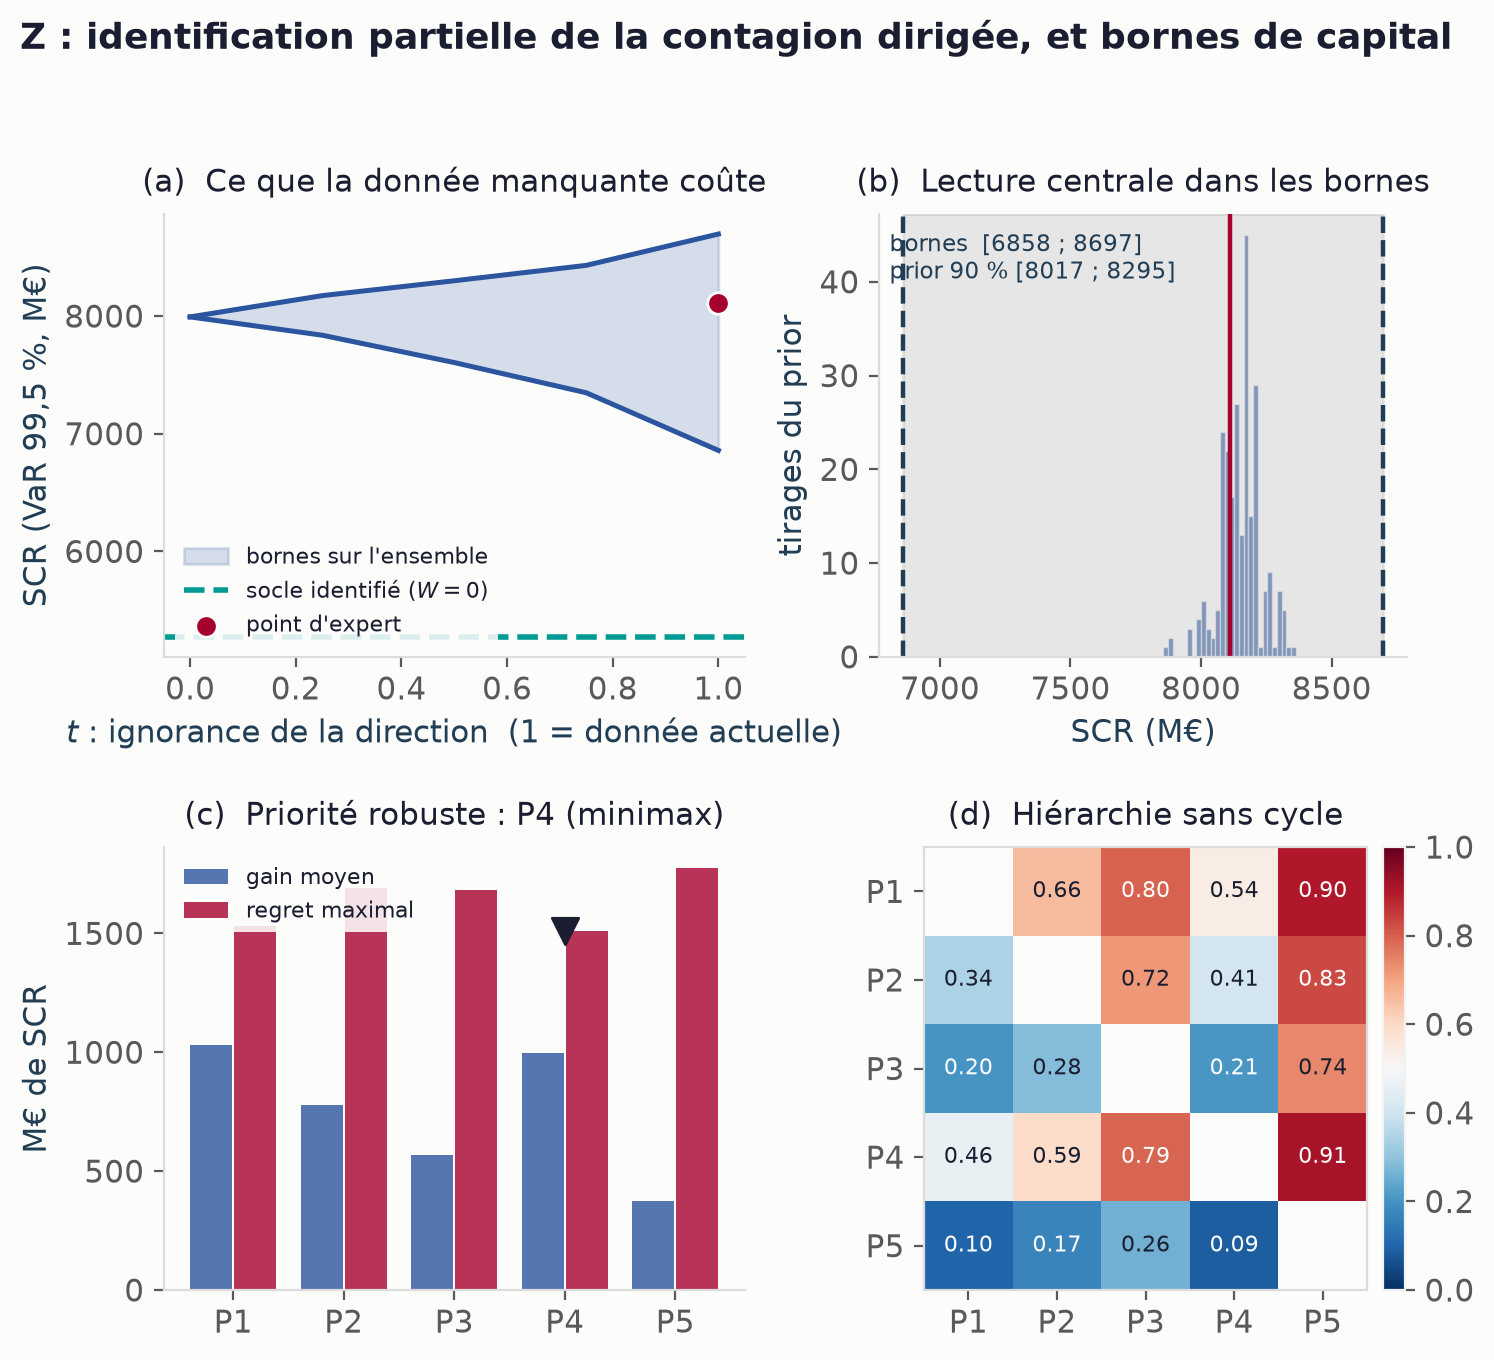
\includegraphics[width=\linewidth]{Z_identification_partielle.png}
\caption{Identification partielle de la contagion dirigée. (a)~Le coût de la donnée
manquante : les bornes se resserrent à mesure que l'ignorance directionnelle $t$ diminue.
(b)~La lecture centrale du prior d'expert, à l'intérieur de bornes qui n'en dépendent pas.
(c)~La priorité de remédiation robuste, au sens du regret maximal. (d)~La dominance
majoritaire entre piliers sur l'ensemble admissible.}
\label{fig:partielle}
\end{figure}

\begin{figure}[htbp]
\centering
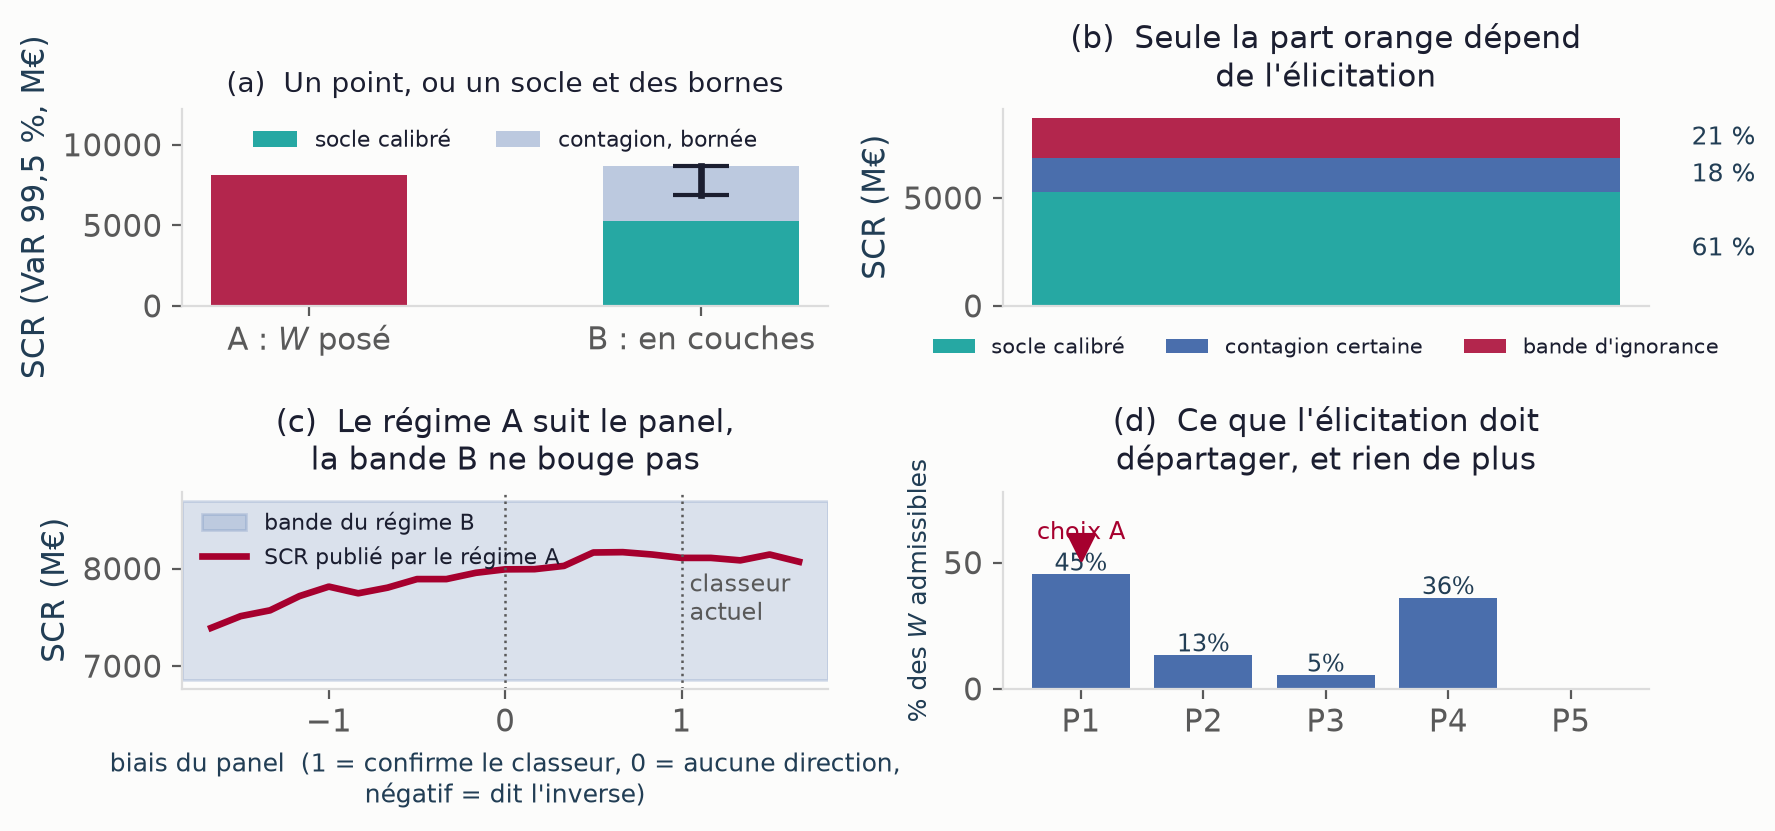
\includegraphics[width=\linewidth]{Z2_comparaison_regimes.png}
\caption{Poser $W$ ou le borner, comparés avant élicitation. (a)~Un point contre un socle
et des bornes. (b)~Seule la part supérieure dépend de l'élicitation. (c)~Le régime~A suit
le biais du panel, la bande du régime~B ne bouge pas. (d)~Ce que l'élicitation doit
départager, et rien de plus.}
\label{fig:regimes}
\end{figure}

\section{L'échelle de repli sur la direction}
\label{sec:echelle-u}

La décomposition $W = S + A$ borne la direction en bloc. On peut faire mieux, en suivant
la méthode d'attaque puis de repli : reparamétrer la propagation par
\[
  \operatorname{logit} p_{ij} \;=\; \operatorname{logit} p_j + u_{ij},
\]
où $p_j$ est l'\textbf{attractivité de la cible} (ce qui subsiste quand la source ne compte
pas) et $u_{ij}$ l'\textbf{excès propre à la source}, c'est-à-dire la direction. La
décomposition n'est identifiée qu'une fois posée la normalisation $\sum_{i\neq j} u_{ij}=0$
pour chaque $j$ : c'est une convention de repérage, et non une information, ce que l'on
vérifie numériquement (une translation compensée de $p_j$ et de $u$ laisse le SCR
strictement inchangé). On descend alors une échelle de crans, du plus ambitieux au repli :
$u$ libre, puis $u$ de \textbf{rang $1$} ($u_{ij}=b_j(a_i-\bar a)$, qui capte $74\,\%$ de
la direction posée et resserre les bornes de $25\,\%$ au prix d'une hypothèse de structure),
puis $u$ élicité, puis $u=0$.

\begin{cle}
\textbf{Le cran nul, et ce qu'il révèle de la contribution.} À $u=0$, la propagation ne
dépend plus que de la cible : \emph{aucune source ne se distingue}. Or c'est exactement là
que P1 et P4, les deux piliers de tête, deviennent \textbf{indiscernables} (gains de
remédiation $1\,051$ contre $1\,052$~M\euro{}, écart nul), alors qu'ils sont séparés de
$353$~M\euro{} dès que la direction du classeur est rétablie. \textbf{La direction est donc
précisément ce qui départage les deux piliers prioritaires} : sans elle, on ne sait plus
lequel remédier d'abord. La contribution du mémoire ne se lit pas sur le niveau d'un
quantile, elle se lit ici, sur une décision qui bascule (figure~\ref{fig:echelle}).
\end{cle}

\begin{figure}[htbp]
\centering
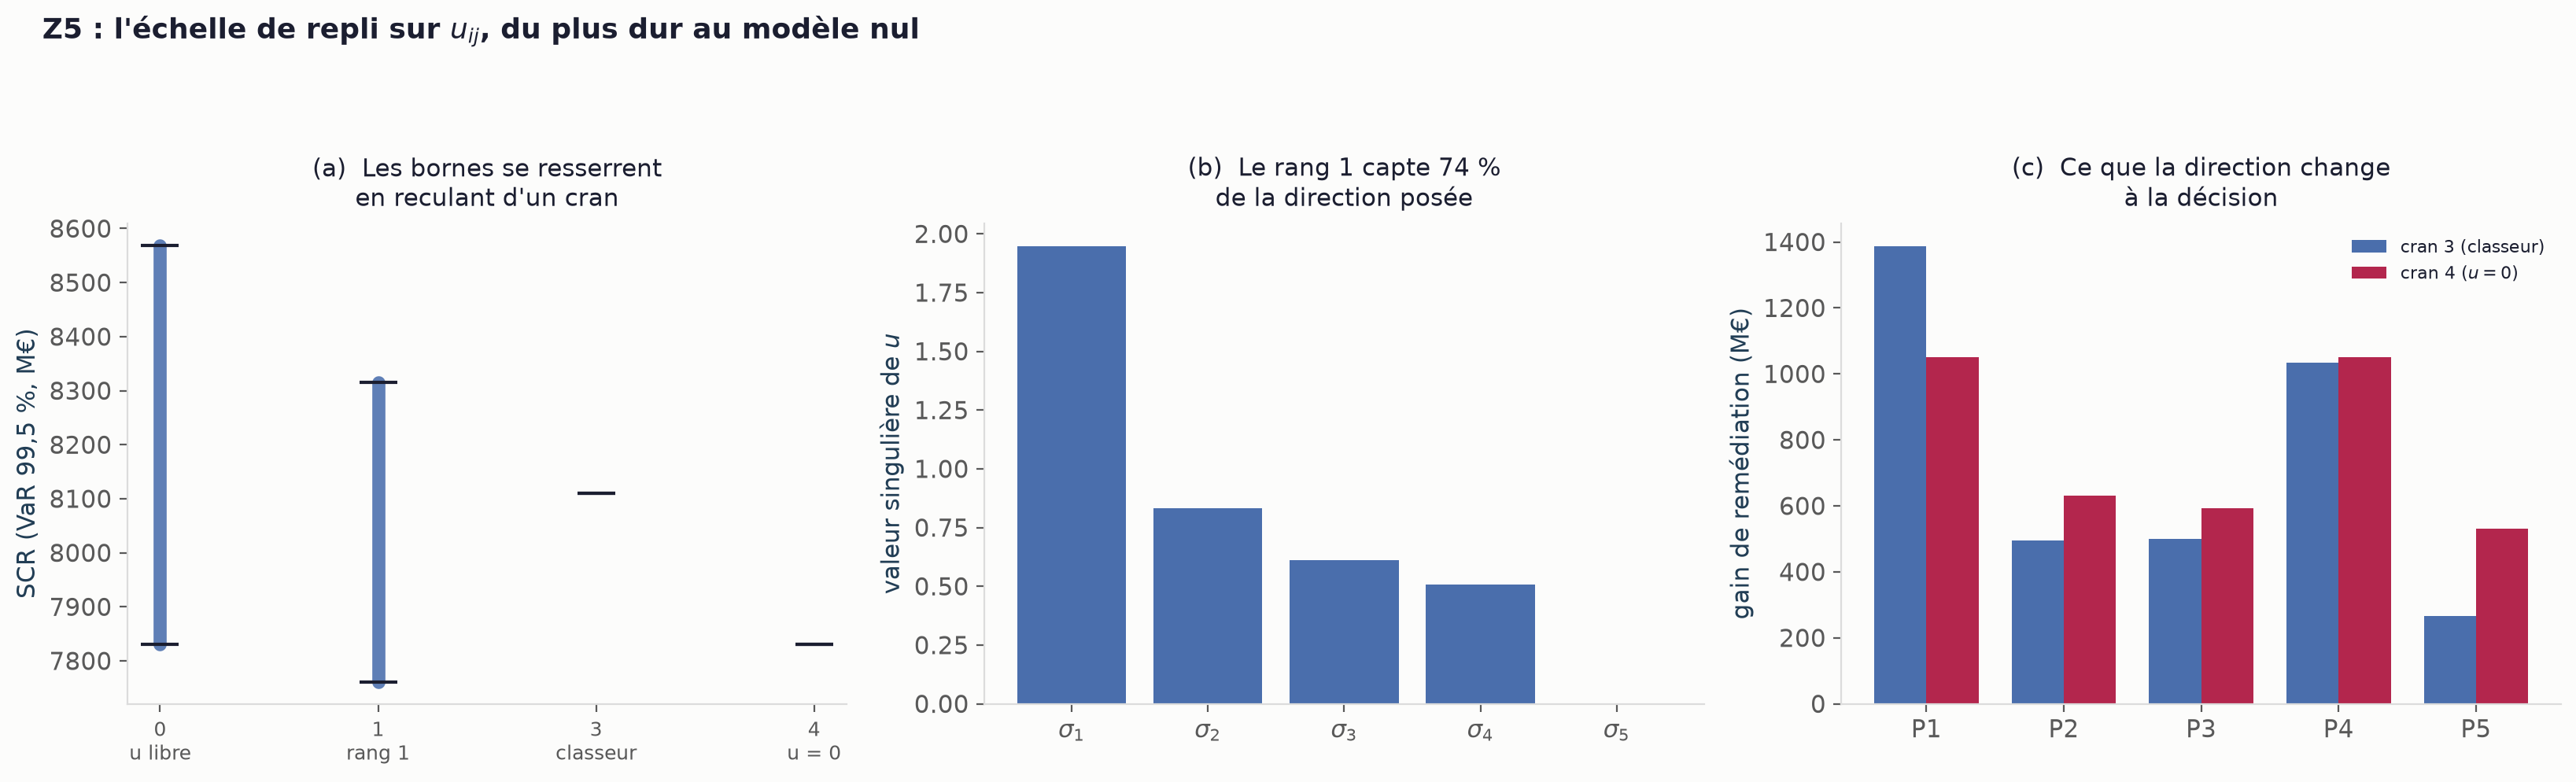
\includegraphics[width=\linewidth]{Z5_echelle_repli.png}
\caption{L'échelle de repli sur $u_{ij}$. (a)~Les bornes de capital se resserrent quand on
recule d'un cran (hypothèse de structure). (b)~Un rang $1$ capte $74\,\%$ de la direction
posée. (c)~Ce que la direction change à la décision : au cran nul, les gains de remédiation
de P1 et P4 se rejoignent.}
\label{fig:echelle}
\end{figure}

% =====================================================================
    % INCHANGÉ, porte la méthode
% FICHIER GENERE PAR construire_v3.py, NE PAS EDITER A LA MAIN.
% Source : chapitres/12_resultats.tex, moins les sections
% retirees, qui restent integralement dans main_v2. Toute correction
% se fait dans le fichier source puis par relance du script, sinon
% les deux divergent.
\chapter{Résultats}
\label{chap:resultats}

Ce chapitre livre le \og combien \fg{} de la question du mémoire, sous la discipline posée
aux chapitres~\ref{ch:identifiabilite} et~\ref{chap:partielle} : les niveaux sont
illustratifs, les écarts et les ordres sont ce qui résiste. Tous les résultats sont ancrés,
comme dans l'ancien mémoire, sur une entité type de $15\,000$~M\euro{} de provisions, avec
deux périmètres de sévérité : OpRisk (grandes pertes opérationnelles, queue lourde)
et PRC (sévérité plafonnée à $40$~M\euro). Sauf mention contraire, on lit la médiane
et l'intervalle interquartile, la variance de la sévérité étant infinie ($\xi\approx0{,}9$).

\begin{attention}
\textbf{Comment lire les niveaux de ce chapitre.} Les montants qui suivent sont
\emph{illustratifs} et ne doivent pas être lus comme la mesure du capital d'une entité réelle.
Le chapitre~\ref{chap:partielle} le démontre : en ne faisant varier que la loi de sévérité et la
fréquence, c'est-à-dire des \emph{entrées} du modèle qui dépendent d'un périmètre de collecte
non transposable, le niveau se déplace d'un facteur $41$, tandis que les rapports au socle
varient d'au plus $33\,\%$ et que le groupe de tête du classement des piliers ne change pas. Le
tableau~\ref{tab:scretat} en donne d'ailleurs l'illustration immédiate : le même état conforme
vaut $8\,301$~M\euro{} sous OpRisk et $2\,589$~M\euro{} sous PRC, soit un facteur~$3{,}2$ pour
un seul changement de périmètre de sévérité. Ce chapitre établit donc des écarts, des
rapports et des ordres, et c'est sur eux, jamais sur un niveau, que reposent ses conclusions.
\end{attention}

\begin{cle}
\textbf{Réconciliation avec le socle du chapitre~\ref{chap:partielle}.} Ce chapitre parle d'un
SCR \emph{conforme} d'environ $5\,900$~M\euro{}, quand le chapitre~\ref{chap:partielle} parle
d'un \emph{socle} de $5\,275$~M\euro{}. Ce ne sont pas deux mesures de la même chose, mais deux
points d'un seul modèle : le socle est pris à contagion nulle ($W=0$), là où l'état
conforme en conserve une. L'ordre socle $<$ conforme $<$ non conforme est donc cohérent, et le
pont terme à terme comme l'écart résiduel de Monte-Carlo sont établis au
\S\ref{sec:ann-reconciliation}.
\end{cle}

% SOURCES-SCRIPTS: 65 66 12 16 63

\section{SCR par état de conformité}

Le SCR croît de façon monotone de l'état conforme à l'état non conforme
(figure~\ref{fig:multietats}). Le tableau~\ref{tab:scretat} donne les trois lectures emboîtées :
la lecture~A (fréquence seule) est directement comparable au mémoire ; la lecture~B ajoute la
propagation de la cascade ; la lecture~C ajoute le canal détection.

\begin{table}[htbp]\centering\small
\renewcommand{\arraystretch}{1.25}
\begin{tabular}{@{}l ccc c ccc@{}}
\toprule
& \multicolumn{3}{c}{\textbf{OpRisk} (M\euro)} & & \multicolumn{3}{c}{\textbf{PRC} (M\euro)} \\
\cmidrule(lr){2-4}\cmidrule(lr){6-8}
État & A & B & C & & A & B & C \\
\midrule
Conforme               & 8301  & 6664  & 5932  & & 2589 & 1903 & 1642 \\
Partiellement conforme & 11059 & 9625  & 9625  & & 3653 & 3118 & 3118 \\
Non conforme           & 15074 & 15074 & 16595 & & 5520 & 5520 & 6577 \\
\bottomrule
\end{tabular}
\caption{SCR par état, trois lectures (A~: fréquence ; B~: $+$~propagation ; C~:
$+$~détection). Le canal détection ne joue qu'aux extrêmes (il
% SOURCES-SCRIPTS: 16
abaisse l'état conforme et relève le non conforme), l'état partiel n'étant pas modulé.}
\label{tab:scretat}
\end{table}

\subsection*{Le chiffre de tête : quatre lectures emboîtées et la lecture publiée}
\label{sec:chiffre-de-tete}

Le tableau qui précède n'est pas le seul protocole du mémoire à chiffrer \og l'écart entre l'état
conforme et l'état non conforme \fg{}. Quatre le font, et ils donnent quatre résultats. Aucun
n'est faux : ils ne relâchent pas le même nombre de canaux entre les deux états, et rien
d'autre ne les sépare. Les publier sans le dire reviendrait à laisser le lecteur trancher sans les éléments.

\begin{center}\footnotesize
\renewcommand{\arraystretch}{1.25}
\begin{tabular}{@{}l c r r r@{}}
\toprule
\textbf{Lecture} & \textbf{canaux} & \textbf{conforme} & \textbf{non conf.} & \textbf{facteur} \\
\midrule
Score de conformité seul, $g$ figé au niveau NC & 1 & 7987 & 16\,847 & $2{,}11$ \\
Fréquence $+$ propagation (lecture~B) & 2 & 6664 & 15\,074 & $2{,}26$ \\
$+$ détection (lecture~C) & 3 & 5932 & 16\,595 & $2{,}80$ \\
\textbf{$+$ accumulation P4 (les quatre canaux)} & \textbf{4} & \textbf{6049} & \textbf{20\,188}
& $\mathbf{3{,}34}$ \\
\bottomrule
\end{tabular}
\end{center}

\vspace{4pt}
\noindent En M\euro, périmètre OpRisk. Les niveaux sont ceux des sorties versionnées ; les
\emph{rapports}, eux, sont recalculés à chaque exécution plutôt que
calculés à la lecture, faute de quoi un niveau amont pourrait bouger sans que le facteur suive.
% SOURCES-SCRIPTS: 25 16 43 67

\begin{cle}
\textbf{Le mémoire publie la lecture à quatre canaux : $6\,049 \to 20\,188$~M\euro, soit un
facteur $3{,}34$ et un écart de $14\,139$~M\euro.} Le motif n'est pas qu'elle donne le chiffre
le plus grand, c'est qu'elle est la seule où l'état conforme est conforme sur tous les
canaux que le modèle possède. Dans la première lecture, l'entité dite conforme propage encore
comme une entité défaillante ; dans les deux suivantes, sa détection ou son accumulation tiers
restent au niveau non conforme. Une entité conforme sur un canal et non conforme sur trois autres
n'est pas un état conforme, c'est une \emph{remédiation partielle}, et la nommer conforme
sous-estime l'écart par construction.

\textbf{Ce qui a changé depuis, et qui permet de trancher.} La version précédente de cet encadré
excluait le canal détection tant que son ampleur n'était pas validée. Elle l'est : il pèse
$2\,928 \pm 343$~M\euro{} en valeur de Shapley et
$4\,562 \pm 819$ en marginal de fermeture, signe résolu sur seize graines.
% SOURCES-SCRIPTS: 68 La réserve qui
justifiait l'attente a donc expiré.

\textbf{Les trois autres lectures ne sont pas retirées}, et c'est délibéré : ce sont des
remédiations \emph{partielles}, ce qui est un objet utile en soi, et leur emboîtement chiffre ce
que coûte de ne fermer qu'une partie des canaux.
\end{cle}

\begin{attention}
\textbf{Le facteur se compare d'une lecture à l'autre, l'écart en euros non}, et il faut le dire
plutôt que de laisser le lecteur le remarquer seul : l'écart passe de $8\,860$ à $8\,410$~M\euro{}
entre les deux premières lignes alors que le facteur monte. La cause n'est pas un effet de modèle
mais un changement de base, l'état conforme passant de $7\,987$ à $6\,664$~M\euro{} d'un
protocole à l'autre. Un écart en euros ne se compare qu'à base égale ; un rapport est sans
dimension. C'est le même motif qui fait publier des élasticités plutôt que des plages au
\S\ref{sec:sensibilite-propagation}.

\textbf{Et la monotonie du facteur s'observe, elle ne se teste pas ici.} Les quatre lignes ne
forment pas une expérience contrôlée, leurs protocoles différant aussi par la graine et par la
base. Elle est \emph{cohérente} avec la super-additivité mesurée sur une autre partition, où
relâcher un canal de plus ajoute son effet propre et les croisés qu'il porte, mais le test de
cette super-additivité est ailleurs, dans les seize configurations des quatre canaux, qui
partagent le même moteur et les mêmes graines.
% SOURCES-SCRIPTS: 68
\end{attention}

\noindent\textbf{Où chaque lecture continue de servir.} Les trajectoires du
\S\ref{sec:res-traj} et la priorisation du \S\ref{sec:res-prio} restent conduites en
\emph{lecture~B}. Ce n'est pas une indécision résiduelle mais un choix d'objet : elles portent
sur l'\emph{ordre} de remédiation, dont le chapitre~\ref{ch:robustesse} montre qu'il est
invariant aux leviers testés, de sorte que le canal ajouté déplacerait leurs niveaux sans
déplacer leur conclusion. Les rejouer relèverait par ailleurs de la recalibration, que le gel
interdit.

\begin{figure}[htbp]\centering
\figover{S10_scr_multi_etats.png}
\caption{SCR par état de conformité (trois canaux emboîtés) et bascule des états en crise
systémique.}
% SOURCES-SCRIPTS: 16
\label{fig:multietats}
\end{figure}

Le surcoût de non-conformité $\Delta_{\text{DORA}}=\mathrm{SCR}(\text{NC})-\mathrm{SCR}(\text{C})$,
à graine Monte-Carlo commune (l'écart ne vient que du changement d'état, non du bruit),
s'obtient par bootstrap deux niveaux (multiplicateurs $+$ sévérité). Il ressort du même ordre
que celui du mémoire, amplifié par la propagation, et $100\,\%$ des tirages sont
positifs.

\begin{table}[htbp]\centering\small
\renewcommand{\arraystretch}{1.25}
\begin{tabular}{@{}l cc c c@{}}
\toprule
& médiane & IC90\,\% & & mémoire (réf.) \\
\midrule
$\Delta_{\text{DORA}}$ NC vs C (OpRisk) & 7401 & $[2830\,;38793]$ & & 3879 \\
$\Delta_{\text{DORA}}$ PC vs C (OpRisk) & 2556 & $[963\,;12768]$  & & --- \\
$\Delta_{\text{DORA}}$ NC vs C (PRC)    & 3668 & $[3201\,;4094]$  & & 2015 \\
$\Delta_{\text{DORA}}$ PC vs C (PRC)    & 1257 & $[1077\,;1466]$  & & --- \\
\bottomrule
\end{tabular}
\caption{Surcoût de non-conformité en euros (M\euro), lecture B (fréquence $+$ propagation),
bootstrap deux niveaux. Côté OpRisk la sévérité de queue est ré-échantillonnée sur les
$91$ excès réels, selon la méthode du mémoire, non tirée dans une approximation
% SOURCES-SCRIPTS: 14
normale~; l'intervalle reste large parce que la queue l'est, non par artefact de méthode.
Le surcoût intermédiaire (PC vs C) est chiffré pour la première fois.}
% SOURCES-SCRIPTS: 16
\label{tab:delta}
\end{table}

\noindent \textbf{Lecture actuarielle.} L'intervalle très large côté OpRisk n'est pas un défaut
du modèle : c'est la signature d'une queue d'indice $0{,}60$, où le niveau du capital est
intrinsèquement imprécis. L'écart typique (interquartile) est bien plus resserré que
l'intervalle à $90\,\%$, et le \emph{signe} du surcoût, lui, est certain. On retrouve la thèse du
mémoire : le SCR est une distribution, pas un point.

\paragraph{L'intervalle PRC est étroit, et il le reste quand on cesse de croire la conversion
exacte.} La sévérité PRC est dérivée du nombre d'enregistrements compromis par la relation
log-log de Jacobs (2014), dont le résidu vaut $0{,}523$ en logarithme naturel : à volume donné,
le coût réel varie d'un facteur $2{,}4$ autour de la droite à $90\,\%$. Réinjecter ce résidu
% SOURCES-SCRIPTS: 21
enregistrement par enregistrement ne rouvre pourtant presque pas l'intervalle, le bruit se
moyennant dans l'ajustement GPD ; il déplace le \emph{niveau} du surcoût de $7\,\%$, sans
l'élargir (\S\ref{sec:ann-jacobs}). L'étroitesse de l'intervalle PRC n'est donc pas un artefact
de la conversion déterministe.

\section{Décomposition par pilier}

En basculant un pilier à la fois de conforme à non conforme, le surcoût se décompose
(figure~\ref{fig:decomp}). Le classement obtenu, $P1>P4>P2>P3>P5$, reproduit exactement
le classement ROOT du modèle qualitatif, établi indépendamment par jugement d'expert : deux
voies de construction distinctes convergent sur la même hiérarchie de piliers.

\begin{figure}[htbp]\centering
\figover{S11_decomp_par_pilier.png}
\caption{Décomposition du $\Delta_{\text{DORA}}$ par pilier et validation croisée avec ROOT.
}
% SOURCES-SCRIPTS: 16b
\label{fig:decomp}
\end{figure}

\begin{cle}
\textbf{Une interaction super-additive, établie là où l'estimateur est fiable.} Les surcoûts
isolés ne somment pas au surcoût total : il reste un terme d'\emph{interaction}, signature de la
cascade (un pilier non conforme amplifie aussi les contagions amorcées ailleurs qui le
traversent), qu'un modèle sans propagation (le LDA à copule du mémoire) ne peut pas produire.
Sa mesure exige toutefois de la prudence : une interaction est une différence de différences,
l'estimateur Monte-Carlo le plus fragile qui soit en queue lourde. Sur la VaR à $99{,}5\,\%$
OpRisk, son \emph{signe n'est pas résolu} : sur six graines à résolution égale
($60\,000$ années chacune), il va de $-137$ à $+1\,395$~M\euro{} et n'est positif que dans
quatre cas sur six, la graine de référence donnant $+1\,395$~M\euro{}. Un estimateur
qui change de signe avec la graine interdit d'en tirer quoi que ce soit. La super-additivité
est en revanche robuste partout où le bruit de queue ne domine pas : en \emph{perte moyenne}
elle est positive sur les six graines ($+532$ à $+659$~M\euro{} OpRisk, $+827$
côté PRC, soit environ un cinquième du surcoût moyen), et jusque dans la VaR du périmètre PRC,
dont le plafond de sévérité tronque la queue ($+905$~M\euro{}). Conséquence pratique : puisque les
marginaux ne somment pas au total, l'attribution du surcoût aux piliers exige une règle
principielle qui somme exactement : c'est l'objet de la valeur de Shapley
(section~\ref{sec:allocation}). À ne pas confondre avec l'interaction entre les quatre
\emph{canaux} de la non-conformité, qui décompose le même écart sur une autre partition, vaut
$+5\,001$~M\euro{} et dont le signe, lui, \emph{est} résolu : elle est reprise terme par terme au
\S\ref{sec:kpi}. Les deux ne s'additionnent pas.
% SOURCES-SCRIPTS: 16b 20b 68
\end{cle}

\section{Allocation du capital : Shapley et Euler}
\label{sec:allocation}

La décomposition qui précède pose deux questions d'allocation distinctes. \emph{Qui porte le
surcoût~?} appelle une attribution par pilier \emph{source} de la non-conformité, qui doit
composer avec l'interaction (les marginaux ne somment pas au total). \emph{Où loge le
capital~?} appelle une allocation du niveau $\mathrm{SCR}(\text{NC})$ par pilier
\emph{touché}, cohérente au sens où les parts somment au total. La valeur de Shapley répond
à la première, la règle d'Euler à la seconde (%
% SOURCES-SCRIPTS: 20
figure~\ref{fig:allocation}).

\subsection{Shapley : attribuer le surcoût, interaction comprise}

On munit les piliers d'une fonction caractéristique
\[
v(S) \;=\; \mathrm{SCR}\bigl(S \text{ en NC},\ \text{reste C}\bigr)-\mathrm{SCR}(\text{tous C}),
\qquad S \subseteq \{P1,\dots,P5\},
\]
calculée par la cascade sur les $2^5$ configurations à graine Monte-Carlo commune. Le
marginal de la section précédente est $v(\{k\})$~; la valeur de Shapley
\[
\varphi_j \;=\; \sum_{S \subseteq \{P1,\dots,P5\}\setminus\{j\}}
\frac{|S|!\,\bigl(5-|S|-1\bigr)!}{5!}\,\bigl[v(S\cup\{j\})-v(S)\bigr]
\]
moyenne la contribution de $j$ sur tous les ordres d'arrivée. Par efficience,
$\sum_j \varphi_j = v(\text{tous}) = \Delta_{\text{DORA}}$ \emph{exactement} : la règle
redistribue l'interaction que les marginaux isolés laissent de côté, quel que soit son signe.

La construction est celle de \citet{Shapley1953}, dont l'efficience est la propriété
axiomatique, et son usage actuariel en allocation de capital sous Solvabilité~II est déjà
documenté \citep{Decupere2011}. Les cinq piliers autorisent l'énumération exacte des $5!$
ordres d'arrivée ; les algorithmes par échantillonnage des permutations
\citep{CastroGomezTejada2009, SongNelsonStaum2016}, indispensables en grande dimension, ne
sont donc pas nécessaires ici, et aucune approximation n'entre dans le tableau qui suit.

\begin{table}[htbp]\centering\small
\renewcommand{\arraystretch}{1.25}
\begin{tabular}{@{}l rrr c rrr@{}}
\toprule
& \multicolumn{3}{c}{OpRisk} & & \multicolumn{3}{c}{PRC} \\
\cmidrule{2-4}\cmidrule{6-8}
pilier & marginal & $\varphi_j$ & part & & marginal & $\varphi_j$ & part \\
\midrule
P1 gouvernance & 3481 & 3717 & $34{,}0\,\%$ & & 1375 & 1608 & $32{,}4\,\%$ \\
P4 tiers       & 2658 & 2810 & $25{,}7\,\%$ & & 1075 & 1252 & $25{,}3\,\%$ \\
P2 incidents   & 1634 & 1867 & $17{,}1\,\%$ & &  721 &  920 & $18{,}6\,\%$ \\
P3 tests       & 1094 & 1484 & $13{,}6\,\%$ & &  571 &  738 & $14{,}9\,\%$ \\
P5 partage     &  665 & 1048 &  $9{,}6\,\%$ & &  311 &  438 &  $8{,}8\,\%$ \\
\midrule
somme          & 9531 & 10\,927 & $100{,}0\,\%$ & & 4052 & 4957 & $100{,}0\,\%$ \\
\bottomrule
\end{tabular}
\caption{Valeur de Shapley du surcoût $\Delta_{\text{DORA}}$ (M\euro, NC vs C, trois canaux,
protocole des trois canaux). Les marginaux somment à $9\,531$ (OpRisk), la valeur de
% SOURCES-SCRIPTS: 16b
Shapley à $10\,927$, le surcoût total exactement. Cellules arrondies au million et parts au
dixième de point, échelle à laquelle la colonne somme exactement à cent : c'est la propriété
d'efficacité de la valeur de Shapley, et elle se lit dans le tableau plutôt que de s'y
excuser en note.}
% SOURCES-SCRIPTS: 20
\label{tab:shapley}
\end{table}

Le classement de Shapley reproduit le classement ROOT sur les deux périmètres. Une part de
cette convergence est mécanique : les amorces de la cascade sont semées
proportionnellement à ROOT (parts $30/27/18/15/9\,\%$),
% SOURCES-SCRIPTS: 20
et le canal fréquence d'un pilier
module sa propre part d'amorce. Le test non trivial est la \emph{déformation} : la part de
Shapley de P1 ($34\,\%$) excède sa part d'amorce ($30\,\%$), effet propre de la propagation
(P1 est l'émetteur le plus fort de $W$), et l'interaction redistribuée ($+1\,395$~M\euro{}
OpRisk, $+905$ PRC à cette graine) est intégralement un produit de la cascade, absent d'un
modèle additif.

\subsection{Euler : allouer le niveau, et une limite d'estimation assumée}

La règle d'Euler alloue $\mathrm{SCR}(\text{NC})$ par
$C_j = \mathbb{E}\bigl[L_j \mid L \ge \mathrm{VaR}_{99{,}5\,\%}\bigr]$ (version TVaR, exacte
par construction), où $L_j$ est la perte du pilier \emph{touché} $j$ dans la cascade. Côté
PRC, l'allocation est stable et presque plate : P2 $23\,\%$, P4 $23\,\%$, P1 $20\,\%$,
P3 $18\,\%$, P5 $17\,\%$, et les parts de capital coïncident avec les parts de perte moyenne
parce que le plafond de sévérité tronque la queue
($\mathrm{TVaR} = 6\,795 \approx \mathrm{VaR} = 6\,573$~M\euro). Côté OpRisk, les parts
\emph{moyennes} sont stables (P2 $23\,\%$, P4 $22\,\%$, P1 $20\,\%$, P3 $18\,\%$,
P5 $16\,\%$), mais l'allocation de la queue extrême ne l'est pas, et la cause en est
théorique : avec $\xi \approx 0{,}6 > 0{,}5$, la sévérité est de variance infinie,
l'estimateur Monte-Carlo de la TVaR converge en régime de loi stable, et le classement
conditionnel bascule d'une résolution à l'autre (vérifié à $150$ et $240$~mille années
simulées). On rapporte donc l'allocation de queue du périmètre PRC, régularisée par le cap,
et l'on tient celle d'OpRisk pour indicative.

\paragraph{La mesure de queue sert ici à \emph{mesurer}, jamais à couvrir.} La distinction est
assez souvent négligée pour qu'il faille l'écrire. Le besoin de capital publié dans ce mémoire
est partout un $\VaR_{99{,}5\,\%}(L)$ centré, conformément au niveau de Solvabilité~II ; aucune
grandeur de couverture n'est une TVaR, ni une CTE, ni un Expected Shortfall. La mesure
de queue intervient à deux titres, et tous deux sont des titres de \emph{diagnostic}. Comme
noyau d'allocation d'abord, dans la règle d'Euler ci-dessus, où elle répartit un niveau déjà
fixé sans le modifier. Comme \emph{indicateur de forme de queue} ensuite : le rapport
$\TVaR_{99{,}5\,\%}(L)/\VaR_{99{,}5\,\%}(L) \approx 2{,}1$ se compare à son asymptote théorique
$1/(1-\xi) = 2{,}5$, et c'est ce rapport, non les deux montants, qui porte l'information.
% SOURCES-SCRIPTS: 67
Ce rapport dépend de l'état et il faut
donc dire lequel : $2{,}10$ vaut à l'état \emph{tous non conforme}, celui de cette section, tandis
que l'annexe~\ref{sec:ann-cte} le mesure à $2{,}17$ sur la calibration de référence. Les deux
% SOURCES-SCRIPTS: 73
valeurs sont justes, elles ne portent pas sur la même loi de perte, et l'écart entre elles est
sans signification en soi.

Deux raisons de ne pas en faire un niveau de couverture, et la seconde est décisive. La
première est de proportion : sur un risque aussi large, dont les queues sont plurielles selon la
catégorie d'événement (chapitre~\ref{chap:adaptations}), adosser la couverture à une moyenne de queue
déformerait la distribution et immobiliserait un capital sans commune mesure avec le niveau
réglementaire de référence. La seconde est d'existence : sous la calibration PRC,
$\hat\xi=1{,}033>1$ place la sévérité en régime d'espérance infinie, et la mesure
n'existe alors pas au sens mathématique. Une mesure de couverture qui cesse d'être définie
selon la source de sévérité retenue ne peut pas porter un besoin de capital ; le même objet,
lu comme un diagnostic de queue, reste au contraire parfaitement informatif, puisque sa
divergence \emph{est} l'information.

\begin{cle}
\textbf{Sources et réceptacles.} Les deux allocations ne racontent pas la même chose, et
c'est le résultat : Shapley, vue \emph{source}, concentre le surcoût sur P1 ($34\,\%$), là
où naît la non-conformité~; Euler, vue \emph{réceptacle}, répartit le capital presque
uniformément sur les piliers touchés (P2 et P4 en tête légère). La remédiation se décide
côté source~; le capital, lui, se loge là où les cascades atterrissent.
\end{cle}

\begin{figure}[htbp]\centering
\figover{S15_allocation_shapley_euler.png}
\caption{Allocation du capital DORA (OpRisk). (a)~Shapley contre marginaux : l'interaction
redistribuée. (b)~Euler : parts de capital (queue) contre parts de perte moyenne~; sur ce
périmètre non plafonné, l'allocation fine de la queue extrême reste indicative
($\xi \approx 0{,}6$, variance de sévérité infinie).}
% SOURCES-SCRIPTS: 20
\label{fig:allocation}
\end{figure}

\section{Trajectoire du capital}
\label{sec:res-traj}

Le long de la mise en conformité, le capital décroît de l'état initial vers le SCR conforme, et
le surcoût résiduel $\Delta_{\text{DORA}}(t)$ tend vers zéro (tableau~\ref{tab:traj},
figure~\ref{fig:traj}). Partant de l'état marginal actuel (NC~$35\,\%$, PC~$35\,\%$, C~$30\,\%$),
le capital OpRisk passe de $\sim 10\,750$ à $\sim 7\,040$~M\euro{} sur cinq ans, vers le SCR
conforme ($\sim 6\,925$).

\begin{table}[htbp]\centering\small
\renewcommand{\arraystretch}{1.2}
\begin{tabular}{@{}c ccc@{}}
\toprule
$t$ (ans) & SCR($t$) médiane & bande 90\,\% & $\Delta_{\text{DORA}}(t)$ \\
\midrule
0 & 10752 & $[9092\,;12654]$ & 3827 \\
1 & 9576  & $[7205\,;12040]$ & 2652 \\
2 & 8310  & $[6194\,;11042]$ & 1385 \\
3 & 7575  & $[5924\,;10164]$ & 650 \\
5 & 7041  & $[5857\,;9028]$  & 116 \\
\bottomrule
\end{tabular}
\caption{Trajectoire du capital DORA (M\euro, OpRisk).}
% SOURCES-SCRIPTS: 17
\label{tab:traj}
\end{table}

\begin{figure}[htbp]\centering
\figover{S12_trajectoire_scr.png}
\caption{Trajectoire SCR($t$) et évolution des états de conformité.}
% SOURCES-SCRIPTS: 17
\label{fig:traj}
\end{figure}

\noindent \textbf{Lecture actuarielle.} L'intégrale de la trajectoire, à un coût de capital
près, est le \emph{coût de portage} de la non-conformité pendant la remédiation. La bande reste
large et surtout haute en environnement dégradé : la vraie exposition n'est pas le capital
médian, c'est le risque que la remédiation traîne quand la menace monte, précisément le scénario
où le capital importe le plus.

\section{Priorisation de la remédiation}
\label{sec:res-prio}

Sous budget contraint (un pilier remédié à la fois), l'énumération des $120$ ordres donne
l'ordre optimal $P1\to P4\to P2\to P3\to P5$, égal à l'ordre ROOT et distinct de l'ordre
glouton par valeur d'accélération (figure~\ref{fig:prio}). L'écart de capital intégré entre le
pire ordre et l'optimal atteint $21\,\%$.

\begin{figure}[htbp]\centering
\figover{S13_priorisation.png}
\caption{Valeur d'accélération par pilier et ordre de remédiation optimal.}
% SOURCES-SCRIPTS: 18
\label{fig:prio}
\end{figure}

\begin{cle}
\textbf{Le myope n'est pas l'optimal.} Remédier au coup par coup le pilier au plus fort gain
immédiat (l'ordre glouton) coûte plus cher que l'ordre optimal, parce que les interactions de
cascade imposent de raisonner sur l'horizon entier. Que l'optimum coïncide avec le classement
ROOT, obtenu par une voie qualitative indépendante, est la troisième convergence
euro~$\leftrightarrow$~ordinal du mémoire, après la stabilité de la progéniture
(\S\ref{sec:branch}) et la décomposition par pilier.
\end{cle}

\paragraph{La question réciproque donne un autre classement, et c'est celui qu'un plan de
remédiation utilise.} Tout ce qui précède fixe un état et lit un capital. L'exercice de
résistance \emph{inverse} fixe le capital et cherche les états qui le produisent, et c'est sous
cette forme qu'un dispositif ORSA emploie un modèle. La monotonie établie au \S\ref{sec:kpi} le
rend court : l'ensemble des configurations atteignant une cible est croissant, donc entièrement
décrit par ses éléments minimaux, et il n'en compte jamais plus de quatre sur seize. Deux nombres
résument alors tout le treillis. Le canal de fréquence seul atteint $10\,377$~M\euro,
soit $1{,}72$ fois l'état conforme, tandis que les trois autres canaux \emph{réunis} n'atteignent
que $11\,413$, soit $1{,}89$ fois. Toute cible sous le premier seuil se produit donc par un canal
unique, et toute cible au-dessus du second exige la fréquence. Aucun autre canal, seul et
dans sa plage déclarée, n'atteint même $8\,000$~M\euro. La lecture directe hiérarchise les canaux
par leur contribution ; la lecture inverse désigne celui dont la maîtrise \emph{interdit} les
scénarios sévères, et ce n'est pas la même information. Détail, frontières par cible et réserves
au \S\ref{sec:inverse}.
% SOURCES-SCRIPTS: 92

\section{Robustesse}

Le niveau du capital bouge fortement selon les leviers non calibrés (l'indice de queue $\xi$
domine, facteur $\sim 6$), mais la direction ($\Delta_{\text{DORA}}>0$) et la
\emph{priorité} (P1 en tête) tiennent sur tous les réglages testés (figure~\ref{fig:robust}).

\begin{figure}[htbp]\centering
\figover{S14_robustesse_multietats.png}
\caption{Robustesse : le classement tient, le niveau non.}
% SOURCES-SCRIPTS: 19
\label{fig:robust}
\end{figure}

\begin{cle}
\textbf{La recommandation ne dépend d'aucun paramètre non mesurable.} L'ordre de remédiation
optimal ne dépend que des SCR par configuration, donc il est invariant aux taux de
transition de la chaîne de Markov, pourtant les paramètres les moins calibrables. Ces taux
fixent le calendrier de la trajectoire, jamais la séquence recommandée. Le verdict d'ensemble
rejoint celui de toute la démarche : le classement est robuste là où le niveau ne l'est pas.
\end{cle}

\begin{attention}
\textbf{Le périmètre exact de cette robustesse.} Les tests ci-dessus font
varier les paramètres du modèle \emph{à matrice $W$ fixée}, celle du classeur qualitatif. Ils
établissent donc que P1 arrive en tête \emph{si l'on admet cette direction}. Dès lors que l'on
admet ne pas connaître la direction et que l'on balaie l'ensemble admissible
(chapitre~\ref{chap:partielle}), P1 et P4 deviennent pratiquement à égalité : P1 arrive
premier dans $43{,}6\,\%$ des configurations, P4 dans $37{,}7\,\%$, et l'écart de regret maximal entre
% SOURCES-SCRIPTS: 30
les deux n'est que de $1{,}5\,\%$. Les deux énoncés ne se contredisent pas, ils portent sur des
sources d'incertitude différentes. Ce qui est robuste dans les deux cadres, c'est que P1 et P4
devancent nettement P2, P3 et P5, et que P5 n'arrive \emph{jamais} en tête.
\end{attention}

\paragraph{Les hypothèses restantes ont leur axe de stress.} Trois entrées ne figuraient pas au
tornado : les coefficients de la conversion Jacobs, la charge systémique $\gamma$ et l'ancrage
des probabilités d'état. Stressées à $\pm 1{,}645$ écart-type, elles déplacent des niveaux sans
jamais toucher la direction ni le classement : le surcoût PRC reste contenu entre $3\,125$ et
$3\,977$~M\euro{} autour du central, $\gamma$ ne commande que la sévérité de la bascule en
crise, et l'ancrage des probabilités d'état déplace le capital espéré actuel mais laisse
inchangés le SCR par état et le surcoût NC contre C, qui lui sont conditionnels. Le détail du
protocole de stress figure au \S\ref{sec:ann-hypotheses}.
% SOURCES-SCRIPTS: 22 67

\section{La sensibilité au niveau de propagation}
% PONT v3 : la section complete est dans main_v2, version
% longue et non modifiee. Genere par construire_v3.py.
\label{sec:sensibilite-propagation}
La crainte que l'on adresse spontanément à un modèle de cascade est que son résultat
dépende du niveau de propagation retenu. La sensibilité mesurée dit l'inverse, et c'est
un résultat contre-intuitif qu'il faut énoncer tel quel : \textbf{le niveau de propagation
est le moins sensible des leviers}, et la fragilité du chiffre se situe dans l'ajustement
de valeurs extrêmes, pas dans la contagion. L'ignorance sur la direction, elle, ne se
stresse pas mais se gradue, et son coût maximal est connu d'avance. Les tables complètes
sont dans la version longue de ce mémoire.

\section{Comparaison de modèles : la dépendance n'est pas le mécanisme}
\label{sec:benchmark}

Le mémoire a remplacé le LDA à copule par la cascade dirigée. Ce que ce remplacement
apporte se mesure en confrontant la cascade à des jumeaux copule construits pour lui
ressembler (figure~\ref{fig:benchmark}, périmètre OpRisk, graines
% SOURCES-SCRIPTS: 23
Monte-Carlo communes). Cette section compare les modèles sur l'axe de la \emph{structure de
dépendance}, à marges fixées ; la comparaison sur l'axe de la \emph{famille de loi} (la bande
de modèle) est conduite en partie~\ref{part:limites}, section~\ref{sec:trois-etages}, et les
deux se complètent.

\textbf{La photo.} À marges par pilier \emph{identiques} (celles de la cascade, état
conforme) et corrélation calée, la copule gaussienne retombe sur le SCR de la cascade
($+0{,}1\,\%$) : en queue lourde ($\xi \approx 0{,}6$), la queue annuelle obéit au principe
de la perte unique dominante et le \emph{niveau} de base n'identifie pas la dépendance. La
Student ($\nu = 4$) le surestime de $17\,\%$ en forçant des co-extrêmes que le mécanisme ne
produit pas ($2{,}28$ piliers extrêmes par année de queue contre $1{,}12$). Le choix de
copule est donc à la fois non identifiable et conséquent~; la cascade n'a pas ce degré de
liberté : sa dépendance est produite par le mécanisme, pas choisie.

\textbf{Et ce résultat a été répliqué ailleurs, sans lien avec ce travail.} L'objection naturelle
serait qu'une coïncidence à $+0{,}1\,\%$ entre une copule gaussienne et un mécanisme de cascade
tient à un réglage particulier du protocole. Le préprint de cascade climatique cité au
chapitre~\ref{ch:positionnement} \citep{ccrn2026} conduit la même expérience, à marges appariées,
entre une gaussienne, une Student et sa propre cascade : il obtient des primes centrales
pratiquement indiscernables et ne voit la séparation apparaître qu'en \emph{queue}. Même
protocole, même conclusion, sur un autre péril et par une autre équipe. Ce n'est donc pas un
artefact du réglage retenu ici, mais une propriété du principe de la perte unique dominante,
qui rend le niveau central aveugle à la structure de dépendance.

\begin{attention}
\textbf{Le $+0{,}1\,\%$ est une graine, et la coïncidence est plus fragile que le nombre ne le
laisse croire.} La reprise du protocole sur quatre graines et un échantillon assez grand pour
qu'un quantile à $99{,}95\,\%$ ait un sens donne, au même niveau
% SOURCES-SCRIPTS: 80
$99{,}5\,\%$, un écart moyen de $+4{,}8\,\%$ d'étendue $10$ points entre graines. Le
$+0{,}1\,\%$ publié n'est donc pas faux, il est \emph{un tirage} : la conclusion à retenir n'est
pas que la gaussienne retombe exactement sur la cascade, c'est que leur écart ne dépasse
pas son propre bruit. L'énoncé faible est le seul qui tienne, et il suffit à l'argument.

\textbf{Et la séparation en queue ne vaut que pour la Student.} Le même protocole, décliné sur
huit niveaux de quantile de $50$ à $99{,}95\,\%$, marque d'une étoile les seules cases où l'écart
dépasse l'étendue entre graines. Au-delà de $99\,\%$, seule la Student sort de son
bruit, à $+20{,}4$, $+29{,}8$ puis $+31{,}2\,\%$ ; ni la gaussienne ni l'indépendance n'y
parviennent, leurs étendues atteignant $13$ et $31$ points. La raison est structurelle : la
Student est la seule des trois à porter une dépendance de queue \emph{asymptotique}. Le préprint
doit donc être cité sur le protocole, jamais sur l'ordre du résultat en queue, qui
dépend de l'indice de queue de la sévérité et non de l'architecture du modèle.
\end{attention}

\textbf{L'intervention.} Basculer un pilier en non-conformité est une intervention, pas un
conditionnement. Le jumeau LDA-copule exprime les canaux fréquence et détection (les marges
dépendent de l'état de leur pilier), mais trois manques sont structurels.
\emph{(i)}~La propagation n'a nulle part où vivre : le surcoût total ressort à
$6\,760$~M\euro{} contre $10\,927$ pour la cascade, une sous-estimation de $38\,\%$.
% SOURCES-SCRIPTS: 67
\emph{(ii)}~Les marges ne dépendant que de l'état de leur propre pilier et la copule étant
figée, la perte moyenne totale est \emph{exactement} additive : interaction moyenne nulle
par construction ($+0$~M\euro{} mesuré), là où la cascade en produit $+560$~M\euro{} :
l'interaction moyenne mesurée plus haut est une signature falsifiable qu'aucun modèle
copule-marges ne peut reproduire. \emph{(iii)}~La priorité de remédiation impliquée
s'inverse sur P2/P3, et la dépendance ne durcit pas quand la conformité se dégrade, alors
que c'est précisément le canal que DORA fait bouger ($g$ de $0{,}45$ à $0{,}90$).

\begin{cle}
\textbf{Le verdict du benchmark.} La copule peut imiter la photo d'un état~; elle ne
peut imiter ni le surcoût (propagation), ni l'interaction (additivité en moyenne), ni le
durcissement de la dépendance avec la non-conformité. La dépendance n'est pas le
mécanisme : c'en est l'ombre portée.
\end{cle}

\begin{figure}[htbp]\centering
\figover{S18_benchmark_copule.png}
\caption{Benchmark copule (OpRisk). (a)~Intervention : le jumeau copule suit les marges et
sous-estime le surcoût, la cascade suit les sources. (b)~Photo : perte unique dominante en
queue~; la Student force des co-extrêmes que le mécanisme n'a pas.}
% SOURCES-SCRIPTS: 23
\label{fig:benchmark}
\end{figure}

\section{Mise en regard réglementaire}

La question finale est celle de la portée : de l'effet de la conformité que le modèle
mesure, quelle fraction les cadres existants savent-ils exprimer ? On confronte donc, sur
le même écart de capital entre profil conforme et non conforme, trois dispositifs.
% SOURCES-SCRIPTS: 27

\begin{table}[htbp]\centering\small
\renewcommand{\arraystretch}{1.25}
\begin{tabular}{@{}l r r@{}}
\toprule
\textbf{Cadre} & \textbf{$\Delta$ capital C$\to$NC} & \textbf{part de l'effet cascade} \\
\midrule
Formule Standard (Solvabilité~II) & $0$~M\euro{} & $0\,\%$ \\
LDA-copule (dépendance symétrique) & $6\,760$~M\euro{} & $62\,\%$ \\
Cascade dirigée & $10\,927$~M\euro{} & $100\,\%$ (référence) \\
\bottomrule
\end{tabular}
\caption{Fraction de l'effet DORA que chaque cadre sait exprimer.}
% SOURCES-SCRIPTS: 27 67
\label{tab:benchmark-sf}
\end{table}

\textbf{La Formule Standard est structurellement aveugle.} La charge de risque opérationnel
$\mathrm{SCR}_{\text{op}} = \min(0{,}3\,\mathrm{BSCR}\,;\,0{,}03\,\max(\text{primes},
\text{provisions}))$ ne dépend que du volume : elle est \emph{identique} pour une entité
exemplaire et pour une entité défaillante sur DORA. Sa réponse à la conformité est nulle par
construction. La copule en capte $62\,\%$ (les canaux fréquence et détection) mais rate la
propagation, faute de direction. Seule la cascade exprime l'effet complet. La valeur du
modèle se lit donc en effet DORA rendu visible, non en un niveau de SCR à
interpréter dans l'absolu.

\begin{cle}
\textbf{Jusqu'où l'open data descend, et où il s'arrête.} Un test sur
% SOURCES-SCRIPTS: 28
la base VCDB montre que les sous-piliers de P2 (familles d'action) et, plus grossièrement,
la détection de P3 sont exploitables sur donnée ouverte (plusieurs centaines d'incidents en
finance, $45\,\%$ de détection lente). Mais le pilier des tiers P4 s'effondre : $56$
incidents à acteur partenaire en finance, et la donnée ouverte sous-code notoirement
l'externalisation. Le pilotage fin de P4 exige donc une donnée que seul un registre
d'externalisation, tenu par l'entité ou le régulateur, peut fournir. C'est le même verdict
que celui du chapitre~\ref{ch:identifiabilite}, décliné au niveau des sous-piliers.
\end{cle}

\begin{figure}[htbp]\centering
\figover{W_benchmark_sf.png}
\caption{Ce que chaque cadre exprime de l'effet DORA : $0\,\%$ pour la Formule Standard,
$62\,\%$ pour la copule, $100\,\%$ pour la cascade.}
% SOURCES-SCRIPTS: 27
\label{fig:benchmark-sf}
\end{figure}

\section{Du secteur à l'entité : ce que la descente d'échelle permet}
% PONT v3 : la section complete est dans main_v2, version
% longue et non modifiee. Genere par construire_v3.py.
\label{sec:ancrage}
Les niveaux établis jusqu'ici valent à l'échelle du secteur. Les transposer à une entité
demande une descente d'échelle, dont les deux canaux, la fréquence et la sévérité, sont
estimés séparément et dont aucun n'a une élasticité de un à la taille. Cette descente a
une \textbf{borne inférieure de validité}, publiée, en dessous de laquelle le modèle
affirmerait qu'une entité de quelques milliards subit à peu près la sévérité d'une
institution mondiale. Le protocole, les élasticités et la borne sont dans la version longue de ce mémoire.

\begin{table}[htbp]\centering
\small
\begin{tabular}{lrrrr}
\toprule
Lecture & $\lambda$ (an$^{-1}$) & sévérité & SCR $99{,}5\,\%$ & Perte moyenne \\
\midrule
Secteur financier mondial & $21{,}56$ & $\times 1$ & $8\,123$~M\euro & $983$~M\euro \\
Seuil \og{}$\geq 10$ événements\fg{} & $0{,}210$ & $\times 1$ & $488$~M\euro & $9{,}7$~M\euro \\
Seuil \og{}toutes firmes\fg{} & $0{,}100$ & $\times 1$ & $229$~M\euro & $4{,}6$~M\euro \\
$\lambda$ lu à la taille de la cible & $0{,}092$ & $\times 1$ & $198$~M\euro & $4{,}3$~M\euro \\
\textbf{Les deux canaux composés} & $\mathbf{0{,}092}$ & $\mathbf{\times 0{,}854}$ &
$\mathbf{169}$~M\euro & $\mathbf{3{,}6}$~M\euro \\
\bottomrule
\end{tabular}
\caption{Le même modèle lu à plusieurs échelles. La matrice $W$ et le moteur de cascade sont
identiques partout ; seules la fréquence d'amorce et l'échelle de sévérité changent. Les deux
dernières lignes sont la lecture cohérente, où la fréquence \emph{et} la sévérité sont prises
à la taille de l'entité visée.}
% SOURCES-SCRIPTS: 60
\label{tab:echelle}
\end{table}

\section{Quatre bilans réels, et le statut du chiffre obtenu}
% PONT v3 : la section complete est dans main_v2, version
% longue et non modifiee. Genere par construire_v3.py.
\label{sec:entites-reelles}
La méthode est appliquée à quatre bilans d'entités réelles, anonymisées en classes de
taille, à partir de leurs seuls états publiés. Le point à retenir n'est pas le montant
obtenu mais son statut : il s'agit d'une \textbf{borne supérieure d'ordre de grandeur et non
d'une mesure}, l'entité notionnelle tombant sous la borne inférieure de validité rappelée
ci-dessus. Le détail des quatre bilans, la table de correspondance des champs et le
motif de la requalification sont dans la version longue de ce mémoire.

\section{Ce que l'agrégation réglementaire fait de cet écart}
\label{sec:agregation-scr}

Les sections qui précèdent chiffrent un besoin et un écart. Il reste à dire ce que le capital
total de l'entité en retient, et la réponse ne va pas de soi. Sous Solvabilité~II, le risque
opérationnel n'entre pas dans la matrice de corrélation du \textsc{bscr} : il s'ajoute,
selon l'identité $\mathrm{SCR} = \mathrm{BSCR} + \mathrm{Adj} + \mathrm{SCR}_{Op}$ posée au
chapitre~\ref{chap:reglementaire}. Un besoin de nature opérationnelle porté en \textsc{orsa} se
transmet donc au capital total sans aucun bénéfice de diversification, et cela vaut du
niveau comme de l'écart entre états. Un euro d'écart \textsc{dora} coûte un euro de capital.

\paragraph{Le contrefactuel, et ce qu'il mesure.} Pour dire ce que cette convention implique, on
agrège le même montant $D$ comme un module de plus, corrélé à $\rho$ avec le \textsc{bscr} pris
comme un bloc. Le taux de reconnaissance vaut alors
\[
  \tau(\rho, d) \;=\; \frac{\sqrt{1 + 2\rho d + d^{2}} - 1}{d},
  \qquad d = \frac{D}{\mathrm{BSCR}},
\]
et son développement en $d = 0$ donne $\tau(\rho, d) = \rho + \tfrac{d}{2}\,(1 - \rho^{2}) +
O(d^{2})$. Un montant petit devant le \textsc{bscr} est donc reconnu à hauteur de $\rho$,
et de $\rho$ seulement, quand la convention additive le reconnaît en entier. L'écart entre les
deux traitements vaut $1 - \rho$ : il ne dépend pas de la taille, et il ne se referme qu'à
corrélation parfaite. Ce contrefactuel n'est pas ce que fait Solvabilité~II ; il sert à
\emph{mesurer} la convention en vigueur, jamais à en proposer une autre.

\paragraph{Ce que la donnée publiée suffit à établir.} Le \textsc{bscr} ne figure pas parmi les
champs retenus, et il n'a pas besoin d'y figurer : $\mathrm{Adj} \le 0$ donne
$\mathrm{BSCR} \ge \mathrm{SCR} - \mathrm{SCR}_{Op}$, et le plafond donne
$\mathrm{BSCR} \ge \mathrm{SCR}/1{,}3$. Minorer le \textsc{bscr} \emph{majore} $\tau$ : les taux
ci-dessous sont donc des majorants, et l'écart entre les deux conventions vaut au moins ce qu'on
y lit.

\begin{center}\small
\renewcommand{\arraystretch}{1.25}
\begin{tabular}{@{}l r r r r@{}}
\toprule
\textbf{Entité} & \textbf{Écart C$\to$NC} & \textbf{$d = D/\mathrm{BSCR}$} &
\textbf{$\tau$ à $\rho = 0{,}25$} & \textbf{additif / corrélé} \\
 & M\euro & & & \\
\midrule
Assureur non-vie A & $34{,}9$ & $0{,}0954$ & $29{,}4\,\%$ & $3{,}41$ \\
Assureur non-vie B & $44{,}4$ & $0{,}0575$ & $27{,}7\,\%$ & $3{,}62$ \\
Assureur vie C & $62{,}7$ & $0{,}0514$ & $27{,}4\,\%$ & $3{,}65$ \\
Assureur vie D & $86{,}0$ & $0{,}0076$ & $25{,}4\,\%$ & $3{,}94$ \\
\bottomrule
\end{tabular}
\end{center}

\vspace{2pt}
\noindent À $\rho = 0{,}25$, la convention additive reconnaît ainsi de $3{,}4$ à $3{,}9$ fois ce
qu'un traitement corrélé retiendrait, et le rapport reste dans cette bande étroite sur un facteur
$134$ de taille de bilan, précisément parce que $\tau$ tend vers $\rho$. Lu sur le niveau plutôt
que sur l'écart, où $d$ est plus grand, le facteur va de $2{,}6$ à $3{,}8$. Rapporté au
\textsc{scr} publié de chaque entité, l'écart entre états pèse de $0{,}58\,\%$ pour la plus grande
à $8{,}21\,\%$ pour la plus petite, et ces points de \textsc{scr} sont acquis en entier.

\paragraph{Le plafond, qui ajoute une borne à la cécité déjà établie.} La charge forfaitaire est
plafonnée à $0{,}3 \times \mathrm{BSCR}$, quelle que soit l'exposition opérationnelle réelle. Sur
l'assureur non-vie~A, dont l'état \textsc{s.25.01} publie un module opérationnel de
$59{,}0$~M\euro, ce plafond vaut $109{,}8$~M\euro{} et la marge restante $50{,}8$~M\euro. Le
besoin calculé, $112{,}1$~M\euro, en représente $2{,}21$ fois, et l'écart entre états,
$34{,}9$~M\euro, en représente $0{,}69$ fois. Autrement dit, même un forfait rendu
sensible à la conformité saturerait avant d'avoir exprimé ce besoin : la Formule Standard n'est
pas seulement insensible, elle est bornée. La lecture $\mathrm{Adj} = 0$ est ici \emph{posée et
déclarée}, un ajustement strictement négatif relevant le \textsc{bscr}, donc le plafond, donc la
marge ; l'état \textsc{s.25.01} de l'entité permet de la lever au cas par cas.

\begin{cle}
\textbf{La lecture décisionnelle, et elle renverse une intuition de gestion.} Un euro économisé
sur la non-conformité \textsc{dora} vaut, en capital, davantage qu'un euro économisé sur un risque
qui se diversifie : le premier est reconnu en entier, le second à hauteur de sa corrélation. Une
direction des risques qui classerait ses chantiers de remédiation au seul vu de la sinistralité
attendue sous-estimerait donc le rendement en capital de celui-ci, d'un facteur de l'ordre de
trois à quatre. Cette conclusion ne dépend d'aucun paramètre du modèle de cascade : elle tient à
la place que le règlement assigne au risque opérationnel, et elle survivrait à un changement
complet de calibration.
\end{cle}

% SOURCES-SCRIPTS: 95 65

\section{Détenir ou transférer, en deux phrases}
% PONT v3 : la section complete est dans main_v2, version
% longue et non modifiee. Genere par construire_v3.py.
\label{sec:detenir-transferer}
Le capital libéré par une remédiation peut être comparé au prix de marché du même risque.
Deux choses en ressortent, et une seule est une sortie du modèle. La valeur présente de
l'économie de portage vaut exactement la variation de capital, quel que soit le taux
retenu : la révision du coût du capital déplace le nombre d'années, pas l'économie. Et
le bénéfice a deux composantes dont une seule est monétisée, la sinistralité évitée
pesant plusieurs fois le portage, si bien que le retour calculé sur le seul portage est
un \textbf{majorant} et non un plancher. Le calcul complet est dans la version longue de ce mémoire.

             % 4 sections retirées

% =====================================================================
\part{Robustesse, limites et perspectives}
\label{part:limites}
% =====================================================================
% FICHIER GENERE PAR construire_v3.py, NE PAS EDITER A LA MAIN.
% Source : chapitres/13_inventaire_hypotheses.tex, moins les sections
% retirees, qui restent integralement dans main_v2. Toute correction
% se fait dans le fichier source puis par relance du script, sinon
% les deux divergent.
% ---------------------------------------------------------------------
% STATUT : RÉDIGÉ (transplanté de exploratory/cascade_qualitative/
%          chapitre_robustesse.tex, préambule retiré).
% FAIT (août 2026) : la ligne u_ij est au tableau des paramètres, avec sa
%          sensibilité mesurée par l'échelle de repli du ch. 10, ainsi qu'une
%          ligne pour l'élasticité sévérité/taille calibrée au ch. 5.
% ---------------------------------------------------------------------
\chapter{Robustesse et incertitude du chiffre reporté}
\label{ch:robustesse}

\noindent Le chapitre~\ref{chap:resultats} a conduit les tests de robustesse eux-mêmes
(tornado, sensibilités, invariance de l'ordre de remédiation). Ce chapitre ne les refait pas.
Il en donne la synthèse en une table, puis pose la question que ces tests laissent ouverte :
une fois l'incertitude reconnue, \emph{quel} nombre reporter. L'inventaire exhaustif des
paramètres, de leur nature et de leur sensibilité, est reporté au \S\ref{sec:ann-parametres}
pour qu'aucun chiffre du mémoire ne soit sans origine déclarée.

\begin{cle}
\textbf{Thèse.} Les conclusions du modèle ne reposent pas sur les paramètres non calibrés.
Je le montre en deux temps : (i)~elles sont insensibles aux choix de modélisation
innocents (structure de la cascade, famille de dépendance, couche temporelle, source de
sévérité) ; (ii)~elles ne réagissent qu'aux leviers qui doivent compter (conformité,
contagion), ce qui est une \emph{qualité}, pas un défaut, c'est la sensibilité au risque que
la Formule Standard n'a pas. Reste une incertitude irréductible, la queue de sévérité, que
j'assume en présentant le SCR comme une distribution, jamais un point.
\end{cle}

\section{L'argument de robustesse, en une table}

\begin{center}\footnotesize
\renewcommand{\arraystretch}{1.3}
\begin{tabular}{@{}p{4.5cm} p{4.6cm} p{4.4cm} c@{}}
\toprule
\textbf{Conclusion} & \textbf{Ce qu'on fait varier} & \textbf{Effet mesuré} & \textbf{Verdict} \\
\midrule
La non-conformité coûte cher ($\Delta_{\text{DORA}}>0$, grand) &
source de sévérité (OpRisk / PRC), famille de copule ($\theta\in[1,4]$) &
facteur ${\sim}1{,}9$ entre sources ; $\Delta_{\text{DORA}}$ varie $<1{,}4\,\%$ sur $\theta$ &
\rob \\
Priorité de remédiation P1 puis P4 (les \emph{sources}) &
cadre de dépendance (cascade vs copule), branchement vs marche &
P1 et P4 en tête dans tous les cadres ; SCR $\pm 4\,\%$ (branchement) &
\rob \\
C'est l'\textbf{asymétrie} de $W$ qui porte le résultat &
knockout de l'asymétrie (3\,000 tirages), placebo directionnel &
sans la direction, le signal tombe sous le bruit du placebo &
\rob \\
Pas de couche de Hawkes &
noyau exponentiel puis à retard, logique two-phase &
excitation intra-journalière (pic $3{,}3$ h) ; endogénéité de $0{,}551$ à ${\sim}0$ si les
co-occurrences du jour passent en exogène &
\rob \\
Les deux lois du socle prédisent une période qu'elles n'ont pas vue &
origine glissante, douze années notées hors échantillon &
fréquence : couverture $91{,}7\,\%$ pour la NB contre $75{,}0\,\%$ pour le Poisson, log-score en
sa faveur ; forme de queue non rejetée ($p=0{,}4087$) &
\rob \\
Le SCR \emph{réagit} à la conformité et à la contagion &
score de conformité $q\in[0,1]$, gain $g\in[0{,}05\,;0{,}90]$ &
$-53\,\%$ de NC à C ; $\times 1{,}6$ sur la plage de $g$ &
\feat \\
Le SCR est une distribution large, pas un point &
incertitude de paramètre (bootstrap deux niveaux) &
facteur ${\sim}2{,}5$ sur la VaR par la seule incertitude de calibration &
\ass \\
Le \emph{niveau} de sévérité ne tient pas hors échantillon &
notation d'une seule année à la fois, seuil ré-estimé sur l'apprentissage &
quantiles dépassés trois fois trop souvent ; l'échelle de queue dérive de $4{,}00\,\%$ par an,
soit au moins $+24{,}7\,\%$ sur le quantile &
\ass \\
Le \emph{signe} de $\Delta_{\text{DORA}}$ ne dépend pas de l'additivité des coûts d'un sinistre &
exposant $\theta\in[0{,}70\,;1{,}30]$ sur le nombre de piliers touchés &
écart de $9\,706$ à $20\,487$~M\euro{} : signe et ordre conservés, \emph{amplitude} non
($76\,\%$ de l'écart publié) &
\ass \\
\bottomrule
\end{tabular}
\end{center}

\vspace{4pt}
\textbf{Lecture.} Les cinq premières lignes sont l'ossature : le signe et l'ordre
de grandeur de l'effet DORA, la hiérarchie des piliers, le rôle de la direction, le statut de
l'auto-excitation et le comportement prédictif des deux lois du socle tiennent quand on change ce
qui pourrait sembler arbitraire. La sixième ligne
n'est pas une fragilité mais le c\oe ur du modèle : un SCR qui ne bougerait pas avec la
conformité serait inutile (c'est le reproche fait à la Formule Standard,
chapitre~\ref{chap:resultats}). Les trois dernières sont les limites honnêtes, et elles ne portent
pas sur le même objet : la queue de sévérité domine l'incertitude sur le \emph{niveau}, donc toute
lecture ponctuelle du SCR serait une surinterprétation ; la dérive de l'échelle de sévérité, seule
limite du mémoire découverte hors échantillon, déplace ce même niveau dans un sens connu et d'une
taille bornée (\S\ref{soc:sec:backtest}) ; l'additivité des coûts d'un sinistre
multi-piliers domine celle qui pèse sur l'\emph{écart}, sans jamais en renverser le signe
(\S\ref{sec:additivite-couts}).

% SOURCES-SCRIPTS: 25 29 47 63 61 66 67 74 08h 89



\section{Les trois étages de l'incertitude du SCR}
\label{sec:trois-etages}

L'incertitude sur le SCR ne se réduit pas au paramètre. Elle se répartit sur trois étages, qu'il
faut nommer plutôt que confondre (figure~\ref{fig:bande-modele}). Le premier est l'incertitude
de paramètre : l'intervalle de confiance de $\xi$ à lui seul dilate la VaR d'un facteur
$2{,}5$ sur la calibration figée, valeur que le bootstrap retrouve à la précision près.
% SOURCES-SCRIPTS: 63 46
Le deuxième est l'incertitude d'identification :
la direction de $W$ n'étant pas identifiable, la contagion se lit en bande
(chapitre~\ref{chap:partielle}). Le troisième, le plus souvent passé sous silence, est
l'incertitude de modèle : le choix de la \emph{famille} elle-même.

On la chiffre en recalculant le SCR sous des familles concurrentes. Sur l'axe de la
\textbf{dépendance}, à marges par pilier fixées, le SCR va de $5\,322$ M\euro{} (indépendance) à
$9\,806$ M\euro{} (comonotone, borne de Fréchet), soit un facteur $1{,}8$, la formule standard
Solvabilité~II et les copules gaussienne et de Gumbel se plaçant entre les deux ; notre cascade
dirigée ($8\,318$ M\euro) tombe dans cette bande, entre une dépendance gaussienne et une
dépendance de Gumbel. Sur l'axe de la famille de queue, l'écart est bien plus large :
d'une lognormale ($4\,330$ M\euro) à une GPD à queue lourde ($\xi=0{,}90$ ; $24\,016$ M\euro),
un facteur $5{,}5$. C'est le choix de la loi de queue qui domine, de loin, l'incertitude de
modèle, et c'est précisément pourquoi le plafond de réassurance ($40$ M\euro) est un levier
distinct, qui ramène la famille lourde à $495$ M\euro : une réponse au risque de queue, non le
risque lui-même.

\begin{figure}[htbp]\centering
\figover{J4_bande_modele.png}
\caption{La bande de modèle, troisième étage d'incertitude. (a)~axe dépendance, à
marges fixées : la cascade se place entre les copules gaussienne et de Gumbel, dans une bande
$[5{,}3\,;9{,}8]$ Md\euro. (b)~axe famille de queue : la queue lourde domine
l'incertitude ($\times 5{,}5$). (c)~les trois étages (paramètre, identification,
modèle) tels que le script les cumule ; la bande \emph{reportée} par le mémoire n'en retient que
les deux premiers, le troisième étant publié comme axe de sensibilité
(\S\ref{sec:etage-modele-hors-bande}).}
% SOURCES-SCRIPTS: 48
\label{fig:bande-modele}
\end{figure}

\subsection{Deux étages se cumulent dans la bande reportée, le troisième en sort}
\label{sec:etage-modele-hors-bande}

Les trois étages ne peuvent pas tous entrer dans un intervalle unique, et il faut dire lequel
en sort et pourquoi. La bande reportée par ce mémoire ne cumule que les deux premiers,
paramètre et identification. L'étage de modèle est publié, mais comme axe de
sensibilité déclaré et non comme composante de la bande.

\paragraph{Les trois étages, mis sur une seule échelle avant toute comparaison.} Comparer les
étages exige de les lire sur la \emph{même} grandeur, et c'est la première chose à faire ici :
l'étage de paramètre est publié sur le quantile d'\emph{un sinistre} (facteur $2{,}5$) tandis que
les deux autres vivent sur la \emph{charge annuelle agrégée}. Les rapprocher tels quels
comparerait deux échelles, ce qui est précisément l'erreur que ce mémoire s'interdit ailleurs.
Porté sur l'agrégat, l'intervalle bootstrap de $\xi$ donne $[3\,042\,;\,27\,152]$~M\euro, soit un
facteur $8{,}93$ : le quantile annuel amplifie l'incertitude de paramètre, et le facteur
$2{,}5$ ne mesure donc pas ce que le paramètre fait au \emph{capital}.
% SOURCES-SCRIPTS: 71

\begin{center}\footnotesize
\renewcommand{\arraystretch}{1.25}
\begin{tabular}{@{}l l r@{}}
\toprule
\textbf{Étage, lu sur la charge annuelle} & \textbf{Bande} & \textbf{Facteur} \\
\midrule
Paramètre ($\xi$ sur son IC$_{90}$) & $[3\,042\,;\,27\,152]$ & $8{,}93$ \\
Identification (direction de $W$) & $[6\,858\,;\,8\,697]$ & $1{,}27$ \\
Modèle, axe dépendance & $[5\,322\,;\,9\,806]$ & $1{,}84$ \\
Modèle, axe famille de queue & $[4\,330\,;\,39\,901]$ & $9{,}21$ \\
\bottomrule
\end{tabular}
\end{center}

\vspace{4pt}
\noindent En M\euro. La hiérarchie ainsi rétablie n'est pas celle qu'on annonce d'ordinaire :
\textbf{l'étage de modèle n'écrase pas les autres}, il est du même ordre que l'étage de paramètre,
et les deux dominent largement l'identification. Le retirer ne peut donc pas se justifier par sa
taille, et l'argument qui suit est d'une autre nature. Réserve à garder : ces largeurs de
paramètre font varier $\xi$ seul, $\sigma$ restant à sa valeur publiée, alors que le bootstrap
estime le couple conjointement ; ce sont donc des \emph{majorants}.

\paragraph{Ce qui justifie le déplacement, et ce n'est pas une taille.} Les deux étages retenus
sont de nature \emph{statistique} : ils mesurent ce que la donnée ne permet pas de trancher à
modèle fixé, et un intervalle est l'objet qui convient pour les porter. Le troisième est
\emph{épistémique} : il mesure l'effet d'un choix de famille, et un choix ne se moyenne pas.

Le point décisif est plus précis que cette opposition générale, et il se voit sur l'axe de la
famille de queue. Cet axe pousse $\xi$ à $0{,}90$, tandis que l'étage de paramètre le fait varier
jusqu'à $0{,}8313$ : c'est le même paramètre, et une bande doit dire \emph{une seule
fois} jusqu'où on le laisse aller. Or $0{,}8313$ est une borne estimée, celle de
l'intervalle bootstrap, quand $0{,}90$ est une valeur posée hors de cet intervalle. Les
placer sur la même échelle met un scénario et une borne de confiance dans le même objet, et le
lecteur ne sait plus si la borne haute est un aléa défavorable ou une autre théorie de la queue.
Le retrait rend la bande homogène, ce qui est un motif plus fort que la lisibilité.

À l'inverse, la borne \emph{basse} de cet axe, la lognormale à $4\,330$~M\euro, est une autre
famille et non un autre $\xi$ : celle-là est un apport propre, et c'est pourquoi le
recouvrement est asymétrique. Le déplacement porte donc sur ce que la bande \emph{annonce},
non sur ce que le mémoire publie.

\paragraph{Où cet étage est publié, désormais.} Il l'est deux fois, et rien n'est caché. Sur
l'axe de la famille de queue, la sixième posture de la table du
\S\ref{sec:predictive-robuste}, le pire cas de modèle à $\xi$ \emph{posé} à $0{,}90$, \emph{est}
l'ambiguïté de famille : c'est le même objet, sous un autre nom, et il porte un chiffre.
Sur l'axe de la dépendance, la bande de $5\,322$ à $9\,806$~M\euro{} reste publiée dans cette
section, avec le repère qui compte, à savoir que la cascade dirigée s'y place entre une
dépendance gaussienne et une dépendance de Gumbel.

\paragraph{Et ce qui ne change pas.} L'ordre d'amorce des piliers reste invariant à la
famille. Le déplacement porte sur la façon de \emph{reporter} le niveau, pas sur la thèse : le
niveau bouge dans la bande, l'ordre résiste, et c'est vrai des trois étages qu'on les cumule
ou non.

\paragraph{Sur l'auto-excitation, une convergence de choix et non une corroboration.} Le parti de
ne pas poser de couche de Hawkes est celui qui prête le plus le flanc, l'auto-excitation étant
devenue l'outil par défaut du cyber. Il est ici adossé à un test contre les variantes de noyau de
la littérature. Le préprint de cascade climatique cité au chapitre~\ref{ch:positionnement}
\citep{ccrn2026} arrive au même endroit, et \emph{pour la même raison de résolution temporelle} :
il retient un graphe acyclique à l'échelle de l'événement, au motif que le processus ponctuel
auto-excité devient naturel lorsque les instants exacts et la rétroaction récurrente sont au
c\oe ur du problème, ce qui n'est pas le cas quand la propagation se joue à l'intérieur d'un
événement dont on n'observe pas la chronologie fine. C'est exactement la situation du présent
travail, et la convergence est d'autant plus notable qu'elle est indépendante : autre péril,
autre équipe, et sans connaissance des travaux sur lesquels s'appuie le test conduit ici.

\begin{attention}
\textbf{Ce que cette convergence vaut, et ce qu'elle ne vaut pas.} Il serait commode de la lire
comme une corroboration du rejet ; ce serait la surinterpréter, et la précision importe puisque
c'est le point le plus exposé du mémoire. Ces auteurs ne testent pas l'auto-excitation contre
leur cascade : ils \emph{posent} le graphe acyclique, et leur mention du processus auto-excité
tient en une ligne d'un tableau de positionnement où il figure comme une représentation mature
parmi d'autres, mieux adaptée à un autre régime d'observation. Ce qui converge est donc le
\textbf{choix de modélisation et son motif}, pas une réfutation. Deux équipes qui ne disposent
pas de la chronologie fine d'un événement écartent le même outil pour la même raison, ce qui
déplace ce parti d'une préférence vers une contrainte d'observation, et c'est tout ce que l'on
peut en tirer. Le rejet lui-même ne repose que sur le test du présent travail.
\end{attention}

\paragraph{Ce que ce test établit réellement : une équivalence observationnelle, et c'est plus
fort qu'un rejet.} Le mot \og rejet \fg{} suppose que la donnée départage les deux modèles. Elle
ne les départage pas, et le mesurer valait mieux que de l'espérer.
% SOURCES-SCRIPTS: 85

L'argument se pose d'abord \emph{sans} rien simuler. Si chaque pilier touché est un événement
enregistrable, la fraction d'événements qui sont des \emph{enfants} vaut
$(\mathbb{E}[k]-1)/\mathbb{E}[k]$, où $\mathbb{E}[k]$ est le nombre moyen de piliers touchés par
sinistre : c'est exactement ce qu'un ajustement de Hawkes appelle son ratio de branchement. Avec
$\mathbb{E}[k]=1{,}931$ à l'état non conforme, une cascade sans aucune auto-excitation
prédit $n=0{,}482$, à comparer au $0{,}551$ mesuré sur la chronologie réelle.

Le test le confirme. On engendre soixante années de dates avec le moteur de cascade, dont la
seule structure temporelle est la durée des pas de propagation \emph{à l'intérieur} d'un sinistre,
puis on lui ajuste un Hawkes exponentiel comme on le ferait sur une chronologie réelle. À la
résolution de la donnée disponible, le jour, l'ajustement trouve $n=0{,}480$, soit la prédiction
analytique à trois millièmes. Il retrouve même l'horloge interne : la demi-vie estimée du noyau
vaut $9{,}0$~h pour un lag de propagation vrai de $6{,}7$~h, et il l'appelle \og décroissance de
l'excitation \fg{}. L'estimateur a été validé au préalable sur un Poisson pur, où il rend
$0{,}004$, et sur trois processus de Hawkes simulés de ratios connus, qu'il retrouve.

\begin{cle}
\textbf{Conséquence, à assumer telle quelle.} Un ratio de branchement de l'ordre de $0{,}5$
mesuré sur des dates réelles ne prouve pas l'auto-excitation : une cascade qui n'en
contient aucune le produit. Les deux modèles sont \emph{observationnellement équivalents} à la
résolution disponible. L'énoncé juste n'est donc pas \og le Hawkes est rejeté \fg{} mais \og le
Hawkes n'est pas distinguable de la cascade, et la cascade est retenue par parcimonie
interprétative \fg{} : elle rend compte du même regroupement temporel par un mécanisme qui porte
en outre la structure inter-piliers et se traduit en capital. C'est une conclusion plus faible en
apparence et plus solide en fait, puisqu'elle cesse de s'appuyer sur un départage que la donnée
ne permet pas.

\textbf{Attention au sens de l'effet de résolution.} Dégrader la résolution fait monter
le ratio estimé, de $0{,}473$ à l'heure jusqu'à $0{,}739$ au mois, parce qu'agréger fabrique du
regroupement apparent. C'est l'opération \emph{inverse} de celle conduite plus haut, qui fait
tomber l'endogénéité en reclassant les co-occurrences du même jour en exogène. Les deux
expériences ne se contredisent pas, elles déplacent deux choses différentes, et les confondre
donnerait une conclusion opposée.
\end{cle}

\begin{cle}
\textbf{Oui, chaque brique a des alternatives.} Fréquence (Poisson, Hawkes, Cox), sévérité
(lognormale, splicing, EVT bayésienne), dépendance (copules, réseaux, Hawkes multivarié),
mesure (TVaR, spectrale, robuste), agrégation (formule standard, Panjer) : on ne prétend pas
détenir \emph{la} méthode. La discipline est ailleurs : on a testé les concurrents les plus
sérieux, on borne l'effet du choix, et surtout le niveau bouge dans la bande mais
l'ordre d'amorce des piliers ne bouge pas ($P1>P4>P2>P3>P5$, invariant à la famille).
Le niveau est illustratif, l'ordre résiste : c'est, chiffrée sur un troisième axe, la thèse du
mémoire, et la réponse à qui demanderait \og et si vous aviez pris une autre méthode~?\fg.
\end{cle}

\section{Quelle grandeur reporter}
% PONT v3 : la section complete est dans main_v2, version
% longue et non modifiee. Genere par construire_v3.py.
\label{sec:predictive-robuste}
\label{sec:posture-retenue}
Une fois l'incertitude établie, il reste à choisir ce que le mémoire publie. Six postures
sont définies et chiffrées, du quantile ponctuel au pire cas à indice de queue posé. La
posture retenue est le \textbf{plug-in accompagné de sa bande}, et le motif est
réglementaire avant d'être d'opportunité : une borne haute sur un ensemble d'ambiguïté est
un suprémum sur une famille de lois, pas un quantile de la loi de perte, donc la
substituer répondrait à une autre question. Un point mérite d'être connu avant d'en
débattre : la posture robuste \textbf{est} la borne haute de l'intervalle déjà publié, de
sorte que reporter le plug-in avec sa bande publie déjà le chiffre robuste. La table des
six postures et leur bruit de simulation sont dans la version longue de ce mémoire.

\section{Un défaut de calibration, chiffré plutôt que corrigé}
% PONT v3 : la section complete est dans main_v2, version
% longue et non modifiee. Genere par construire_v3.py.
\label{sec:pu-coherence}
La calibration publiée porte une incohérence arithmétique connue : le taux de dépassement
et le nombre d'excès ne désignent pas le même échantillon, alors que la formule qui les
emploie n'a que deux degrés de liberté pour trois entrées. L'effet est \emph{calculé} et
non estimé, il vaut quelques pour cent sur le quantile unitaire, soit une fraction de la
largeur de l'intervalle publié sur cette même grandeur. La valeur reste gelée, et ce choix
est assumé : rejouer un pipeline stochastique pour un écart de cette taille déplacerait
des centaines de nombres publiés sans qu'aucun déplacement soit attribuable à la
correction, et la piste d'audit serait perdue pour un gain immatériel.

\textbf{Deux prudences à ne pas confondre.} Côté solvabilité l'écart est
anti-conservateur, il sous-estime le capital, et une sous-estimation se déclare ; côté
thèse il va dans l'autre sens, le chiffre avancé étant minoré et non gonflé. Seul le
premier engage. Le calcul, son signe et le contrôle qui le recalcule à chaque exécution
sont dans la version longue de ce mémoire.

\section{Défaillances simultanées et additivité des coûts}
\label{sec:additivite-couts}

La cascade produit, pour chaque sinistre, un \emph{ensemble} de piliers touchés, si bien que la
défaillance simultanée n'est pas un cas particulier resté de côté mais la sortie même du modèle. La
loi exacte de ce nombre est donnée au \S\ref{sec:ann-additivite} : à l'état non conforme, la
défaillance multiple est majoritaire, $62{,}31\,\%$ des sinistres touchant plus d'un
pilier contre $31{,}15\,\%$ à l'état conforme. Reste la question de l'agrégation
des coûts, et elle demande de distinguer trois énoncés que le seul mot d'additivité recouvre.

\begin{enumerate}[leftmargin=*,itemsep=2pt]
\item \textbf{Au sein d'un sinistre}, les coûts des piliers touchés \emph{s'additionnent} : c'est
une hypothèse de construction, non testée, et c'est le seul des trois que la question met en cause.
\item \textbf{En fonction des piliers non conformes}, le capital est \emph{presque additif},
$R^2=0{,}9945$ sur les $32$ configurations : c'est une mesure, et elle explique qu'une structure de
dépendance entre états ne déplace pas le capital espéré (\S\ref{sec:ann-dependance-etats}).
\item \textbf{En fonction des quatre canaux}, il est \emph{franchement super-additif},
$+5\,001$~M\euro{} d'interaction sur $14\,139$, soit $+35\,\%$ (chapitre~\ref{chap:resultats}) :
c'est également une mesure.
\end{enumerate}

\noindent Répondre \og~le modèle est super-additif~\fg{} serait donc faux : il l'est sur les canaux,
pas sur les piliers, et l'hypothèse sur les coûts d'un incident est un troisième objet.

\paragraph{Ce que la première coûte, chiffré plutôt que supposé.} On la relâche par un exposant, la
perte d'un sinistre touchant $k$ piliers valant $\bigl(\sum_j X_j\bigr)k^{\,\theta-1}$, de sorte que
$\theta=1$ redonne exactement le modèle publié et que les sinistres mono-pilier restent intouchés.
Pour $\theta$ parcourant $[0{,}70\,;1{,}30]$, l'écart entre états parcourt
$[9\,706\,;20\,487]$~M\euro, soit $76\,\%$ de l'écart publié et $15$~fois son bruit de simulation de
$\pm 734$~M\euro. L'effet est donc réel, et l'additivité des coûts est la plus lourde des
hypothèses structurelles non testées du modèle. Deux précautions pour ne pas en tirer un classement
qu'il n'établit pas : elle porte sur l'\emph{écart} là où la queue de sévérité domine l'incertitude
sur le \emph{niveau} (\S\ref{sec:trois-etages}), et c'est une hypothèse de structure et non un choix
de prudence, les trois choix posés du \S\ref{sec:pu-coherence} déplaçant davantage mais dans une
direction connue.

\paragraph{Elle n'est pas neutre entre les deux états, ce qui n'était pas attendu.} Les élasticités
valent $0{,}95$ à l'état non conforme contre $0{,}39$ à l'état conforme, un facteur $2{,}42$, parce
que l'exposant ne mord que sur les sinistres multi-piliers, majoritaires au seul état non conforme.
L'hypothèse interagit donc avec le canal de propagation au lieu de s'ajouter à côté de lui,
et atteint de ce fait la grandeur centrale du mémoire et non un simple niveau. Ce qui tient malgré
tout : sur toute l'amplitude examinée l'écart garde son signe et son ordre de grandeur, jamais
proche de zéro, si bien que la thèse ne dépend pas de l'hypothèse d'additivité et que seule son
amplitude en dépend. C'est la structure d'argument déjà employée pour les valeurs de $g$.

Le \emph{sens} de la non-additivité, lui, n'est pas déterminable : mutualisation de la remédiation
et saturation de la capacité de réponse tirent en sens contraire, et aucune source ne les sépare. Le
détail, la loi du nombre de piliers, la table complète des exposants et la raison pour laquelle
l'amplitude est posée plutôt qu'estimée sont au \S\ref{sec:ann-additivite}.

\vspace{2pt}
% SOURCES-SCRIPTS: 74 68 69


\begin{cle}
\textbf{La double lecture.} \og Insensible aux choix innocents, sensible aux leviers réels \fg :
le modèle n'est ni sur-ajusté ni fragile, il est piloté par ce qui doit le piloter.
Et la seule grande incertitude, la queue, est nommée et bornée, pas cachée. C'est ce qui
transforme \og je n'ai pas tout calibré \fg{} en \og je sais précisément de quoi mon SCR
dépend, et de quoi il ne dépend pas \fg.
\end{cle}

% =====================================================================
 % 2 sections retirées
\chapter{La donnée manquante comme livrable, hiérarchisé}
\label{ch:livrable}

\begin{cle}
\textbf{Idée directrice.} Le chapitre~\ref{ch:identifiabilite} a montré que la direction de la
contagion n'est pas identifiable sur les sources agrégées. Cette limite n'est pas un point final :
elle se retourne en \textbf{spécification de reporting}, et cette spécification se \textbf{chiffre}
puis se \textbf{hiérarchise}. C'est la contribution réglementaire du travail, et elle ne dépend
d'aucun prior.
\end{cle}

\section{Ce qu'un registre devrait contenir}

Puisque les deux sources agrégées échouent pour des raisons \emph{opposées} (l'une manque de
taxonomie et de volume informatif, l'autre de résolution temporelle), la donnée qui identifierait
$W$ se déduit par complémentarité. Un registre d'incidents \textsc{tic} l'identifiant devrait :
\begin{enumerate}[itemsep=2pt]
\item horodater la \textbf{survenance} (et non la seule déclaration) au \textbf{mois ou à la
      semaine}, afin de porter une antériorité que le pas annuel efface ;
\item catégoriser par \textbf{domaine de contrôle} (les piliers DORA), et non par vecteur
      d'attaque, afin qu'une transition soit interprétable comme un lien $k \to j$ ;
\item consolider une \textbf{cause commune} comme \emph{un} événement à $N$ victimes, pour ne pas
      confondre un lot de déclaration avec une contagion séquentielle.
\end{enumerate}

Ces trois exigences ne sont pas hors d'atteinte : le registre d'information imposé par
l'\emph{implementing technical standard} du règlement d'exécution \citep{eu2024_2956} porte déjà
l'identification des prestataires, la chaîne de sous-traitance et la criticité des fonctions. Ce
qui manque relève du \emph{format} de l'horodatage et du \emph{choix de la taxonomie}, non d'une
collecte nouvelle.

\section{Ce que cette information vaut, en capital}

Une recommandation de reporting reste un v\oe u tant qu'elle n'est pas chiffrée. On la chiffre en
restreignant l'ensemble admissible du chapitre~\ref{chap:partielle} aux configurations compatibles
avec l'information acquise, puis en mesurant le rétrécissement de la bande de capital.

\begin{definition}[Valeur d'information d'une contrainte]\label{def:voi}
Soit $\mathcal{W}$ l'ensemble admissible et $\mathrm{SCR}:\mathcal{W}\to\R_+$ la fonctionnelle de
capital. La largeur de bande associée à un sous-ensemble $\mathcal{V}\subseteq\mathcal{W}$ est
\begin{equation}
  L(\mathcal{V}) \;=\; \sup_{W\in\mathcal{V}}\mathrm{SCR}(W)\;-\;\inf_{W\in\mathcal{V}}\mathrm{SCR}(W).
  \label{eq:largeur-bande}
\end{equation}
Une information $\mathcal{I}$ qui restreint l'ensemble à $\mathcal{W}_{\mathcal{I}}\subseteq
\mathcal{W}$ a pour \textbf{valeur} le rétrécissement relatif qu'elle produit :
\begin{equation}
  V(\mathcal{I}) \;=\; 1-\frac{L(\mathcal{W}_{\mathcal{I}})}{L(\mathcal{W})} \;\in\;[0,1].
  \label{eq:voi}
\end{equation}
\end{definition}

Cette définition a deux propriétés utiles. Elle est \textbf{monotone} : si
$\mathcal{I}'$ implique $\mathcal{I}$, alors $\mathcal{W}_{\mathcal{I}'}\subseteq
\mathcal{W}_{\mathcal{I}}$ et donc $V(\mathcal{I}')\ge V(\mathcal{I})$, une information plus
riche ne pouvant pas valoir moins. Et elle est \textbf{sans dimension}, donc indépendante du
niveau de capital, ce qui la rend comparable d'une source de sévérité à l'autre alors même que
ce niveau, lui, varie d'un facteur quarante.

Le corpus de sept rapports post-incident du chapitre~\ref{ch:identifiabilite} établit le
\emph{sens} de six des dix dépendances entre piliers. À lui seul, il fait tomber la largeur de la
bande de $\mathbf{66\,\%}$. C'est la valeur, en capital, de la lecture de sept documents publics,
et elle donne l'ordre de grandeur de ce qu'un registre correctement spécifié apporterait.

\begin{attention}
\textbf{Ce qu'aucune information de sens ne donnera.} Même les dix directions établies, une bande
subsisterait, imputable à la seule \textbf{amplitude} des coefficients : connaître le sens d'un
lien ne donne pas sa force. L'identification partielle n'est donc pas un état provisoire que la
donnée finirait par lever, elle est \textbf{structurelle}. C'est une raison de plus de lire le
capital en bande, et de ne pas promettre à un superviseur davantage que ce qu'un registre peut
tenir.
\end{attention}

\section{Quelle dépendance documenter en priorité}

L'apport le plus actionnable est ailleurs que dans le total. En fixant le sens d'\emph{une seule}
dépendance à la fois, on obtient un \textbf{classement} des données manquantes par valeur
d'information (figure~\ref{fig:voi}). L'écart est considérable : documenter la seule dépendance
entre gouvernance et gestion des incidents lèverait à elle seule $\mathbf{28{,}9\,\%}$ de
l'ambiguïté de capital, tandis que documenter le lien entre tests et tiers n'en lèverait
\emph{rien}.

Deux conséquences pratiques. D'abord, un superviseur qui ne pourrait exiger qu'une seule
dépendance sait désormais laquelle demander, et une entité qui ne pourrait instrumenter qu'un seul
lien sait lequel instrumenter. Ensuite, un fait qui oriente la recommandation : \textbf{la
dépendance la plus précieuse est précisément celle que le corpus documentaire ne couvre pas}. La
lecture de rapports publics a livré ce qu'elle pouvait livrer ; le reste exige la donnée d'entité.

\begin{figure}[htbp]
\centering
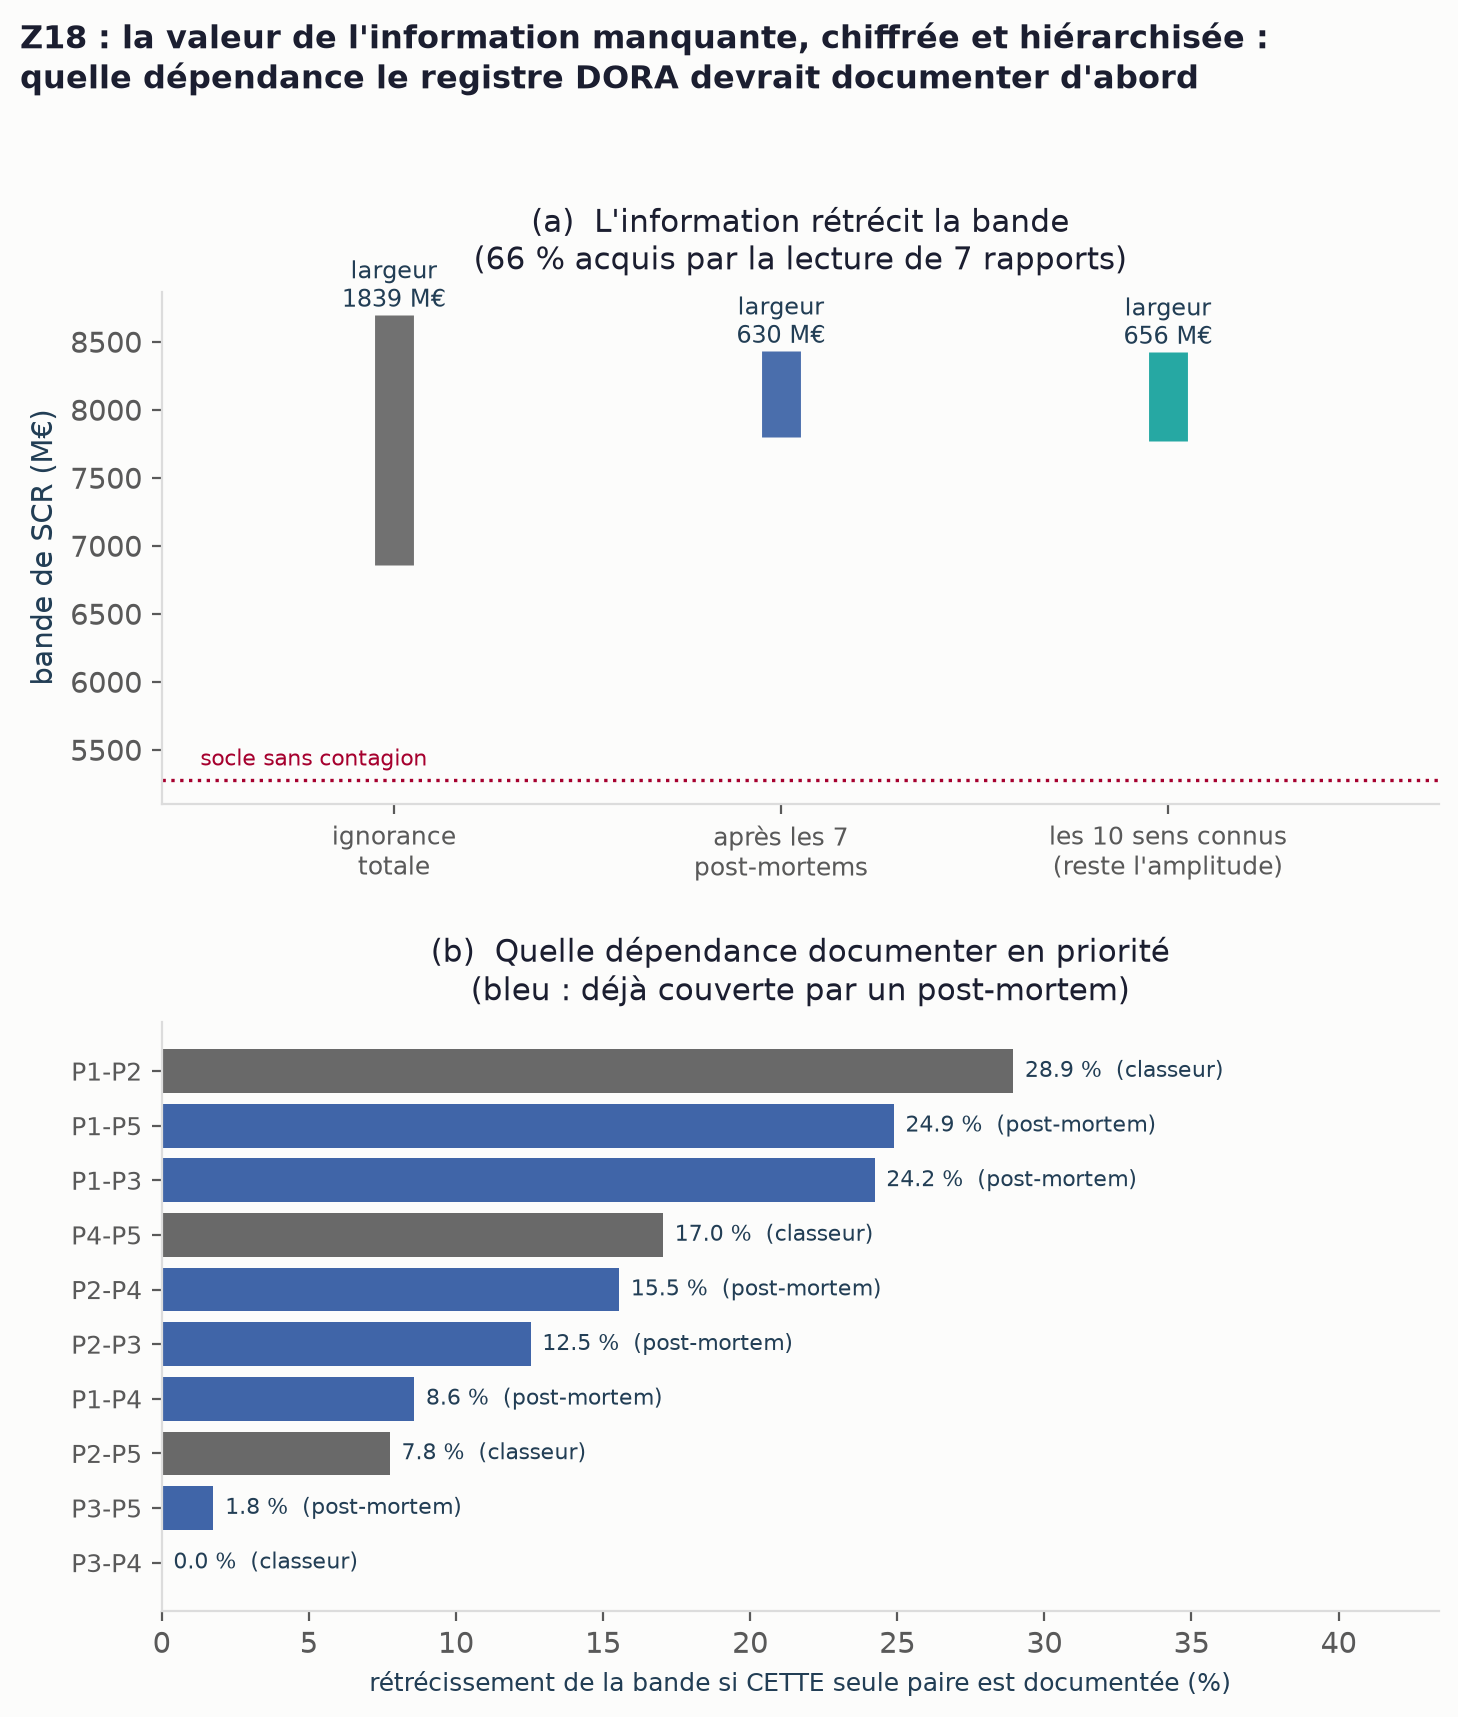
\includegraphics[width=\linewidth]{Z18_valeur_information.png}
\caption{La valeur de l'information, chiffrée et hiérarchisée. (a)~l'information rétrécit la
bande de capital : $66\,\%$ acquis par la lecture de sept rapports, et une bande d'amplitude qui
subsisterait même les dix sens connus. (b)~quelle dépendance documenter en priorité ; en bleu,
celles que le corpus couvre déjà. Source : script~\texttt{55}.}
\label{fig:voi}
\end{figure}

\begin{cle}
\textbf{La limite devenue contribution.} Un mémoire qui se contenterait de constater qu'il ne
peut pas calibrer $W$ laisserait le lecteur sans suite. En spécifiant la donnée qui manque, en
chiffrant ce qu'elle vaut et en la hiérarchisant, on transforme une frontière d'identification en
\textbf{recommandation opposable}, adressée au cadre de reporting que DORA met précisément en
place. C'est le seul endroit du mémoire où une limite produit un livrable.
\end{cle}

% =====================================================================
  % INCHANGÉ, contribution réglementaire
\chapter{Conclusion}

Ce mémoire a construit un modèle interne partiel du coût en capital de la non-conformité à
DORA, où la dépendance entre les cinq piliers est portée par une cascade dirigée plutôt que
par une copule, et où le capital dépend de l'état de conformité de l'entité. Trois lignes de
résultat s'en dégagent, et ce qui est acquis se dit ici aussi nettement que ce qui
ne l'est pas.

\section{Ce qui est établi}
\paragraph{Le chiffre.} Entre l'état conforme et l'état non conforme sur les quatre canaux, le
besoin de capital passe de $6\,049$ à $20\,188$~M\euro{} à l'échelle du secteur, soit un facteur
$3{,}34$. Les canaux isolés en expliquent $9\,138$~M\euro{} et leur interaction $5\,001$, soit
$35\,\%$ de l'écart : un plan de remédiation doit donc citer l'effet de fermeture d'un canal et
non son effet isolé. La fréquence est le levier qui commande : seule, elle porte le besoin de
capital à $10\,377$~M\euro{}, et toute cible au-delà de $11\,413$~M\euro{} l'exige. Ce montant
reste un besoin de capital au sens de l'ORSA, non un SCR réglementaire.

\paragraph{Le mécanisme.} Le mécanisme tient et se distingue formellement de ses concurrents : la criticité dépend de
l'ordre de propagation, propriété qu'aucune dépendance symétrique ni aucun score
additif ne peut reproduire, et la normalisation de Leontief garantit la stabilité de la
contagion, cycles compris, par construction et non par calibration heureuse. Sur les marges
que la donnée fixe, la queue de sévérité ($\hat\xi = 0{,}5954$ au seuil publié), la
fréquence d'entrée et l'accumulation par cause commune, l'ancrage empirique est solide, et il est
éprouvé hors échantillon : la loi de comptage et la forme de la queue passent le backtest, le
niveau de la charge annuelle ne le passe pas pour une raison mesurée, la dérive de l'échelle de
sévérité. Le processus de Hawkes n'est pas distinguable de la cascade à la résolution
disponible ; il est écarté par un choix de parcimonie argumenté, non par un test qui le
réfuterait. Enfin, le modèle exprime intégralement l'effet de la
conformité sur le capital là où la Formule Standard n'en exprime rien.

\paragraph{Un acquis de méthode, qu'il faut compter comme tel.} Chaque nombre publié dans ce
mémoire est confronté, section par section, aux sorties versionnées des scripts que cette section
cite, et le contrôle rend séparément ce qu'il confirme, ce qu'il exempte avec son motif et ce
qu'il ne confirme pas. Il porte aujourd'hui sur la totalité des nombres du document, sans zone
non couverte autre que celles qui sont déclarées avec leur raison. Ce n'est pas une coulisse
d'atelier : le dispositif a trouvé trois valeurs fausses qu'aucune relecture n'avait vues, toutes
justes au moment où elles avaient été écrites et devenues fausses quand une valeur amont avait
bougé. Il est décrit au \S\ref{sec:ann-harnais}, avec ce qu'il ne garantit pas, car il ne vérifie
ni qu'un nombre est au bon endroit ni qu'il veut dire ce que la phrase prétend.

% SOURCES-SCRIPTS: 28 39 43 68 92 47 89 91 85

\section{Ce qui est démontré comme non mesurable}
La direction de la contagion n'est pas identifiable sur les données publiques. Le
mémoire l'établit sur trois sources qui échouent pour des raisons distinctes, résiste à la
tentation du test dégénéré du temps inversé, et pousse jusqu'à la meilleure expérience
naturelle disponible, le choc de chaîne d'approvisionnement MOVEit, dont l'effet net
s'annule une fois un placebo retranché. Le troisième échec ferme la dernière échappatoire :
le schéma \textsc{veris}, standard de description d'incidents adopté par la profession, porte
littéralement les deux champs manquants, et leur intersection n'est renseignée que dans
\emph{un} incident sur $10\,591$. Le problème n'est donc pas de savoir quoi collecter, il est
d'en rendre le remplissage obligatoire. Cette limite n'est pas dissimulée, elle est
convertie en méthode : le capital est borné sur l'ensemble des matrices admissibles plutôt
qu'appuyé sur une matrice posée. Le socle sans contagion est ainsi défendable sans aucune hypothèse non
identifiable, et la contagion ajoute une bande explicite au-dessus de ce socle.

% SOURCES-SCRIPTS: 30 34 28

\section{Ce qui en découle pour le régulateur}
La donnée qui rendrait la contagion mesurable se déduit par complémentarité des trois échecs :
un registre d'incidents horodatant la survenance à la semaine, catégorisant par
domaine de contrôle et non par vecteur d'attaque, consolidant une cause commune
comme un événement unique, et consignant l'ensemble des piliers touchés par chaque incident,
dont la loi jointe distingue à elle seule une matrice de sa transposée. Les deux premières exigences sont déjà des champs normalisés du
schéma \textsc{veris} : la recommandation ne demande donc pas d'inventer une taxonomie, elle
demande d'en rendre le remplissage obligatoire, ce que la notification d'incident
majeur sous DORA peut imposer et qu'une base déclarative volontaire ne peut pas. Cette
spécification n'est pas un v\oe{}u : le mémoire chiffre en euros de capital le resserrement des
bornes qu'elle apporterait, et la hiérarchise par dépendance. La limite d'identifiabilité
devient une recommandation de reporting opposable, ce qui donne au travail une portée
au-delà du modèle.

\section{Ce qui en découle pour l'entité}
Le capital n'est pas seulement un chiffre à publier, c'est un coût. En le confrontant au prix
de marché du même risque, le mémoire met les trois leviers d'une entité, remédier, détenir,
transférer, sur un seul axe en euros par an. À l'échelle d'entité, le coût annuel de détention
vaut plus de deux fois la sinistralité attendue, un traité en excès de perte correctement
dimensionné réduit le coût total d'au plus deux tiers environ, borne supérieure que la capacité
du marché, les exclusions et le risque de contrepartie entament, et la remédiation déplace ce point
d'équilibre en plus d'abaisser le capital. Le niveau reste illustratif, et il l'est doublement
puisque la descente d'échelle du secteur vers l'entité passe par deux élasticités estimées.
Mais le \emph{rapport} entre coût de détention et prix de transfert résiste mieux que le
niveau, et pour une raison qui est une identité plutôt qu'une mesure : ses deux termes
sont proportionnels au \emph{même} SCR, qui se simplifie, de sorte qu'un changement d'échelle
pur le laisse inchangé. Il vaut $2{,}78$ au taux de la directive et $3{,}51$ au taux
historique. Ce qui subsiste est un effet de forme, la descente d'échelle déplaçant la
fréquence et la sévérité séparément plutôt que de redimensionner la loi de perte, et le seul
balayage disponible le borne par le haut à $+36\,\%$ sur une plage de SCR d'un facteur quatre.
C'est la lecture décisionnelle que le travail visait, et elle est plus robuste que le niveau
sans être invariante.

% SOURCES-SCRIPTS: 58 65 67

\section{Limites, sans détour}
L'élicitation structurée est préparée et non exécutée (annexe~\ref{ch:elicitation}) : la
lecture centrale de la direction repose donc sur un classeur qualitatif, non sur une agrégation
d'experts pondérée. Deux hypothèses pèsent le plus sans être testables sur la donnée : les
niveaux de propagation, posés, et l'additivité des coûts entre piliers touchés, dont
l'élasticité vaut $0{,}95$ à l'état non conforme contre $0{,}39$ à l'état conforme
(\S\ref{sec:additivite-couts}). Dans les deux cas le signe et l'ordre de l'écart résistent à
toute la plage étudiée, non son amplitude. Le
niveau absolu du SCR est illustratif et ne doit pas être cité hors de son cadrage relatif.
L'incertitude de queue domine toute lecture ponctuelle, ce qui impose de présenter le capital
en distribution. Et l'ordre de remédiation entre les deux piliers de tête, la gouvernance et
la gestion des tiers, dépend de la direction non identifiée : le mémoire sait dire que ces
deux-là dominent, pas lequel remédier d'abord sans un dire d'expert.

% SOURCES-SCRIPTS: 74

\section{Ouvertures}
Trois prolongements se dessinent : mener l'élicitation structurée pour resserrer la bande
directionnelle sur ses deux degrés de liberté restants ; approfondir le pilier des tiers sur
des données clients, là où l'open data s'effondre ; et passer de la sensibilité de
propagation à une véritable criticité au sens de l'audit, c'est-à-dire au risque résiduel
après mesures de contrôle, une fois disponible une métrique de mitigation par pilier.

% =====================================================================
                  % INCHANGÉ

% =====================================================================
\appendix
% PAS DE \addcontentsline ICI. preambule_v2 redefinit \part par titlesec en style
% [display], et dans cette configuration titlesec ecrit LUI-MEME l'entree de
% sommaire d'un \part*. La ligne explicite que porte main.tex en ajouterait une
% seconde, defaut constate sur la v2 le 9 septembre 2026.
\part*{Annexes}
% =====================================================================
% LES ANNEXES SONT INCHANGEES ET TOUTES CONSERVEES. La reduction porte sur le
% corps, pas sur elles : une annexe retiree ne serait pas condensee, elle serait
% perdue, et l'Institut demande explicitement que les developpements usuels y
% figurent.
\chapter{Démonstrations : le modèle de cascade}
\label{ann:cascade}

% HARNAIS-HORS-SCRIPT: chapitre de demonstrations de la cascade : memes constantes d'enonce ; les valeurs numeriques correspondantes sont verifiees au chapitre cascade, qui cite ses scripts.

Cette annexe démontre les propriétés énoncées à la section~\ref{sec:formalisation}. Les
notations sont celles du chapitre~\ref{chap:cascade} : $P=\{1,\dots,5\}$, $W\in[0,1]^{P\times P}$
avec $W_{jj}=0$, et la cascade indépendante de la définition~\ref{def:cascade}.

\section*{Forme réduite et descendance espérée (proposition~\ref{prop:reduite})}

\begin{proof}
Soit $\mathcal M_n(a,k)$ le nombre de marches dirigées de longueur $n$ de $a$ vers $k$ dans le
graphe pondéré. Une marche $a=v_0\to v_1\to\cdots\to v_n=k$ est vivante avec probabilité
$\prod_{t} W_{v_{t-1}v_t}$, ces arêtes étant indépendantes ; en sommant sur les marches,
$\mathbb E\,\mathcal M_n(a,k)=\sum \prod_t W_{v_{t-1}v_t}=(W^n)_{ak}$ par définition du produit
matriciel. Le nombre de fois où $k$ est atteint depuis $a$ en comptant \emph{chaque} chemin
vaut $\sum_{n\ge0}\mathcal M_n(a,k)$, d'espérance $\sum_{n\ge0}(W^n)_{ak}$. Cette série
matricielle est la série de Neumann de $W$ ; elle converge vers $(I-W)^{-1}$ si et seulement si
$\rho(W)<1$, auquel cas $\sum_{n\ge0}W^n=(I-W)^{-1}$.

L'indicatrice $\mathbf 1\{k\in S_a\}$ vaut $1$ dès qu'\emph{au moins un} chemin vivant relie
$a$ à $k$, donc $\mathbf 1\{k\in S_a\}\le \sum_{n\ge0}\mathcal M_n(a,k)$ presque sûrement. En
prenant l'espérance puis en sommant sur $k$,
\[
  \mathbb E\,|S_a|=\sum_k \mathbb P(k\in S_a)\le \sum_k\bigl((I-W)^{-1}\bigr)_{ak}
  =\bigl[(I-W)^{-1}\mathbf 1\bigr]_a .
\]
L'inégalité est stricte dès qu'un pilier est accessible par plusieurs chemins avec probabilité
positive, ce qui quantifie les collisions.
\end{proof}

\section*{Sous-criticité par normalisation (proposition~\ref{prop:leontief})}

\begin{proof}
Par construction~\eqref{eq:norm}, $W=(g/s_{\max})\,\mathrm{TRANS}\ge 0$ et, pour toute ligne
$j$, $\sum_k W_{jk}=(g/s_{\max})\sum_k \mathrm{TRANS}_{jk}\le (g/s_{\max})\,s_{\max}=g$, puisque
$s_{\max}$ est la plus grande somme de ligne de $\mathrm{TRANS}$. Pour une matrice à
coefficients positifs, le rayon spectral est majoré par toute norme d'opérateur subordonnée,
en particulier la norme infinie, qui est le maximum des sommes de lignes :
$\rho(W)\le\lVert W\rVert_\infty=\max_j\sum_k W_{jk}\le g<1$. La série de Neumann converge donc
et $(I-W)^{-1}=\sum_{n\ge0}W^n$ existe, à coefficients positifs.
\end{proof}

\section*{Loi exacte de l'ensemble atteint (proposition~\ref{prop:loi})}

\begin{proof}
Fixons $A\ni a$. L'événement $\{S_a=A\}$ est l'intersection de deux événements portant sur des
arêtes disjointes, donc indépendants : (i) aucune arête ne relie $A$ à son complémentaire (sans
quoi $S_a$ dépasserait $A$), et (ii) $a$ atteint tout $A$ par les seules arêtes internes à $A$.
L'événement (i) ne concerne que les arêtes $j\to k$ avec $j\in A$, $k\notin A$, chacune absente
avec probabilité $1-W_{jk}$ indépendamment ; sa probabilité est $B(A)=\prod_{j\in A,k\notin A}(1-W_{jk})$.
L'événement (ii) ne concerne que les arêtes internes à $A$ ; notons $R(A)$ sa probabilité.
Par indépendance, $\mathbb P(S_a=A)=R(A)\,B(A)$.

Pour $R(A)$, on partitionne selon le sous-ensemble $A'$ effectivement atteint par les arêtes
internes : $A'$ contient $a$, et $A'\subsetneq A$ est \emph{propre} si et seulement si $A$
n'est pas entièrement atteint. Or, conditionnellement à ce que l'ensemble atteint par les
arêtes internes soit exactement $A'$, aucune arête ne va de $A'$ vers $A\setminus A'$, événement
de probabilité $\prod_{j\in A',k\in A\setminus A'}(1-W_{jk})$ et indépendant de la réalisation
interne à $A'$. En sommant les probabilités de ces sous-ensembles propres et en passant au
complémentaire,
\[
  R(A)=1-\sum_{\substack{A'\subsetneq A\\ a\in A'}} R(A')\!\!\prod_{j\in A',k\in A\setminus A'}\!\!(1-W_{jk}),
\]
avec $R(\{a\})=1$. La récursion sur les sous-ensembles emboîtés est finie et détermine $R$ de
proche en proche.
\end{proof}

\section*{Monotonie stochastique (proposition~\ref{prop:mono})}

\begin{proof}
On construit un \emph{couplage}. Soit $(U_{jk})$ une famille de variables uniformes sur $[0,1]$
indépendantes, commune aux deux matrices. Pour une matrice $M$, déclarons l'arête $j\to k$
vivante si $U_{jk}<M_{jk}$ ; le graphe obtenu a la bonne loi (arête vivante avec probabilité
$M_{jk}$). Si $W\le W'$ terme à terme, alors $U_{jk}<W_{jk}\Rightarrow U_{jk}<W'_{jk}$ : toute
arête vivante sous $W$ l'est sous $W'$. Le graphe sous $W$ est donc un sous-graphe de celui sous
$W'$, et l'accessibilité étant croissante par ajout d'arêtes, $S_a(W)\subseteq S_a(W')$ presque
sûrement. Pour toute fonctionnelle $\varphi$ croissante pour l'inclusion,
$\varphi(S_a(W))\le\varphi(S_a(W'))$ p.s., d'où la domination stochastique et la monotonie de
l'espérance et des quantiles. Enfin, pour une perturbation antisymétrique $A$, l'entrée $W_{jk}$
croît quand $W_{kj}$ décroît : les deux effets jouent en sens contraire sur $S_a$, la monotonie
en $A_{jk}$ n'a plus lieu, et l'optimum sur le pavé $\{|A_{jk}|\le t\,S_{jk}\}$ doit être
cherché aux sommets sans garantie qu'ils le réalisent.
\end{proof}

\section*{Dépendance à l'ordre et non-identification (propositions~\ref{prop:ordre} et~\ref{prop:nonid})}

\begin{proof}
\emph{Ordre.} Soit $\sigma=(i_1,\dots,i_n)$ et $\sigma'$ une permutation de $\sigma$. Alors
$\ell(\sigma)=\ell(\sigma')$ pour toute paire si et seulement si le produit
$\prod_k \mathrm{TRANS}_{i_k i_{k+1}}$ ne dépend pas de l'ordre des facteurs disponibles, ce qui,
pour $n=2$, équivaut à $\mathrm{TRANS}_{ij}=\mathrm{TRANS}_{ji}$ pour tout $(i,j)$, soit la
symétrie de $\mathrm{TRANS}$. La contraposée donne le résultat : $\mathrm{TRANS}$ asymétrique
implique l'existence d'une paire dont l'ordre change la vraisemblance, donc la criticité n'est
pas une fonction de l'ensemble. Toute copule et tout score additif étant symétriques en leurs
arguments, aucun ne reproduit cette dépendance.

\emph{Non-identification.} La décomposition $W=\tfrac12(W+W^\top)+\tfrac12(W-W^\top)=S+A$ est
unique car $S$ est symétrique, $A$ antisymétrique, et cette somme directe est celle des
matrices en parties symétrique et antisymétrique. La co-occurrence observée d'une paire
$\{j,k\}$ est, par échange des rôles, une fonction de $W_{jk}+W_{kj}=2S_{jk}$ seulement ; de
même la statistique d'asymétrie du placebo compare $M$ à sa transposée et son espérance sous
permutation ne dépend que de $S$. Donc $W$ et $W^\top=S-A$ induisent les mêmes lois observables
de co-occurrence. Ils diffèrent par le signe de $A$, et la proposition~\ref{prop:mono} montre
qu'un tel changement modifie l'ensemble atteint, donc le SCR, en général : la direction est non
identifiée.
\end{proof}

\section*{Efficience de la valeur de Shapley}
\label{sec:ann-efficience-shapley}

Le chapitre~\ref{chap:resultats} attribue le surcoût de capital aux piliers par la valeur de
Shapley, et lit dans le tableau que la colonne des parts somme exactement à cent. Cette somme
n'est ni une coïncidence ni un artefact d'arrondi : c'est la propriété d'\textbf{efficience}
\citep{Shapley1953}, et elle se démontre en quelques lignes. Elle est reproduite ici parce que
c'est elle, et elle seule, qui autorise à présenter une attribution comme une \emph{partition} du
surcoût et non comme une pondération arbitraire.

\begin{proposition}[Efficience]
\label{prop:efficience}
Soit $v$ une fonction caractéristique sur $\{1,\dots,n\}$ avec $v(\emptyset)=0$, et
\[
  \varphi_i \;=\; \frac1n \sum_{u \subseteq -\{i\}} \binom{n-1}{|u|}^{-1}
                  \bigl[v(u \cup \{i\}) - v(u)\bigr].
\]
Alors $\sum_{i=1}^{n} \varphi_i = v(\{1,\dots,n\})$.
\end{proposition}

\begin{proof}
La démonstration repose entièrement sur la réécriture du poids. Pour $|u|=s$,
\begin{equation}
  \frac1n \binom{n-1}{s}^{-1} \;=\; \frac1n \cdot \frac{s!\,(n-1-s)!}{(n-1)!}
  \;=\; \frac{s!\,(n-s-1)!}{n!},
  \label{eq:poids-shapley}
\end{equation}
de sorte que $\varphi_i$ est exactement la moyenne, sur les $n!$ \textbf{permutations} de
$\{1,\dots,n\}$, de la contribution marginale de $i$ à l'ensemble de ses prédécesseurs. En effet,
un sous-ensemble $u$ de cardinal $s$ ne contenant pas $i$ est l'ensemble des prédécesseurs de $i$
dans exactement $s!\,(n-s-1)!$ permutations : $s!$ ordres pour les éléments de $u$, puis
$(n-s-1)!$ pour ceux qui suivent $i$. En notant $\Pi$ l'ensemble des permutations et $P_i(\pi)$
les prédécesseurs de $i$ dans $\pi$,
\[
  \varphi_i \;=\; \frac{1}{n!} \sum_{\pi \in \Pi}
              \bigl[v\bigl(P_i(\pi) \cup \{i\}\bigr) - v\bigl(P_i(\pi)\bigr)\bigr].
\]
Sommons alors sur $i$ \emph{à permutation fixée}. Si $\pi = (\pi(1),\dots,\pi(n))$, les
ensembles de prédécesseurs emboîtés donnent
$P_{\pi(j+1)}(\pi) = P_{\pi(j)}(\pi) \cup \{\pi(j)\}$, si bien que la somme des contributions
marginales le long de $\pi$ est \textbf{télescopique} :
\[
  \sum_{i=1}^{n} \bigl[v\bigl(P_i(\pi)\cup\{i\}\bigr)-v\bigl(P_i(\pi)\bigr)\bigr]
  \;=\; \sum_{j=1}^{n} \bigl[v\bigl(P_{\pi(j+1)}(\pi)\bigr)-v\bigl(P_{\pi(j)}(\pi)\bigr)\bigr]
  \;=\; v(\{1,\dots,n\}) - v(\emptyset),
\]
et cette valeur ne dépend pas de $\pi$. En moyennant sur les $n!$ permutations,
$\sum_i \varphi_i = v(\{1,\dots,n\})$, puisque $v(\emptyset)=0$.
\end{proof}

\paragraph{Ce que l'efficience garantit, et ce qu'elle ne garantit pas.}
Elle garantit que l'attribution est une partition \emph{exacte} du surcoût, quelle que soit
l'interaction et quel que soit son signe : rien n'est perdu ni dupliqué. Elle ne garantit
\textbf{pas} que la part d'un joueur soit une prédiction de ce qu'on obtiendrait en l'écartant
seul, laquelle est la contribution \emph{marginale} et ne somme pas au total. C'est la distinction
que le chapitre~\ref{chap:resultats} tient entre les trois lectures d'un même canal, et l'annexe
des adaptations par pilier en donne l'identité correspondante pour chaque colonne. En particulier,
une part de Shapley est une \emph{convention} d'attribution défendable, non un budget de
remédiation : deux des quatre canaux du modèle sont bornés et non calibrés.

\paragraph{Pourquoi aucun échantillonnage n'est nécessaire ici.}
La réécriture~\eqref{eq:poids-shapley} est aussi ce qui rend le calcul praticable : elle ramène
l'évaluation à une moyenne sur les permutations, forme sur laquelle reposent les algorithmes
d'approximation en temps polynomial \citep{CastroGomezTejada2009, SongNelsonStaum2016},
indispensables dès que la dimension croît. Avec cinq piliers, les $5!$ permutations et les $2^5$
valeurs de $v$ sont énumérées exhaustivement : les valeurs publiées sont donc exactes au bruit de
simulation de $v$ près, et aucune erreur d'approximation combinatoire ne s'y ajoute.

  % Démonstrations : cascade
\chapter{Démonstrations}
\noindent Les preuves de stabilité de la cascade ($\rho(W)<1$ par normalisation de Leontief) et
de la propriété de branchement figurent au chapitre~\ref{ch:proprietes}, avec leur vérification
numérique. Cette annexe rassemble les démonstrations de la théorie des valeurs extrêmes sur
lesquelles s'appuie la calibration de sévérité.

% MIGRÉ AUTOMATIQUEMENT depuis memoire/main.tex (plages 3155-3164, 3181-3216).
% Hiérarchie descendue d'un cran, labels préfixés "soc:".
% RELECTURE FAITE (août 2026). Contenu purement EVT, aucun résidu de l'ancien
% modèle. DEFAUT CORRIGE : les cinq labels se suivaient sans unite de
% sectionnement, si bien que les cinq renvois du ch. 6 resolvaient tous vers le
% MEME numero (celui du chapitre). Chaque demonstration a desormais sa section.
\section{Théorème de Fisher-Tippett-Gnedenko}
\label{soc:ann:ftg}
La loi limite $H$ des maxima normalisés est \emph{max-stable} : $H^t(x)=H(a_tx+b_t)$ pour tout $t>0$. En posant $g(x)=-\ln H(x)$, la max-stabilité devient l'équation fonctionnelle $t\,g(a_tx+b_t)=g(x)$. Sa résolution (via la théorie des fonctions à variation régulière de Karamata) impose $g(x)=(1+\xi x)^{-1/\xi}$, soit $H=H_\xi$. Le domaine d'attraction se caractérise ensuite par le comportement de queue : $F\in\mathrm{DA}(H_\xi)$ avec $\xi>0$ si et seulement si $\bar F$ est à variation régulière d'indice $-1/\xi$, i.e.\ $\bar F(tx)/\bar F(x)\to t^{-1/\xi}$. Les lois lognormale et gamma relèvent du cas $\xi=0$ (Gumbel) ; les lois à support borné du cas $\xi<0$ (Weibull).


\section{Théorème de Pickands-Balkema-de Haan}
\label{soc:ann:balkema}
Pour $F\in\mathrm{DA}(H_\xi)$, il existe une fonction positive $a(\cdot)$ telle que, pour $y\ge0$,
$\lim_{u\to x_F}\bar F(u+y\,a(u))/\bar F(u)=(1+\xi y)^{-1/\xi}$.
Or $\bar F(u+ya(u))/\bar F(u)=\Prob(X>u+ya(u)\mid X>u)=1-F_u(y\,a(u))$, dont la limite est la survie GPD $\bar G_{\xi,1}(y)$. En posant $\sigma(u)=a(u)$, on obtient $F_u(y)\to G_{\xi,\sigma(u)}(y)$. La convergence est uniforme car les $F_u$ sont des fonctions de répartition monotones convergeant vers une limite continue (théorème de Pólya). Le paramètre $\xi$ est préservé car il gouverne à la fois la variation régulière de $\bar F$ et la forme de la GPD limite.



\section{Information de Fisher et normalité asymptotique de l'EMV de la GPD}
\label{soc:ann:fisher}
On part de la log-vraisemblance \eqref{soc:eq:loglik-gpd}, écrite par observation avec $W_i=1+\xi Y_i/\sigma$ :
\begin{equation}
\ell_i(\xi,\sigma)=-\ln\sigma-\Bigl(1+\tfrac1\xi\Bigr)\ln W_i.
\end{equation}

\paragraph{Moments-clés.} La transformation de probabilité intégrale donne $W_i^{-1/\xi}=\bar G(Y_i)\sim\mathcal U(0,1)$, donc $W_i\overset{d}{=}U^{-\xi}$ avec $U\sim\mathcal U(0,1)$. On en déduit les quatre moments qui suffisent au calcul :
\begin{equation}
\E[W^{-1}]=\E[U^{\xi}]=\tfrac{1}{1+\xi},\quad
\E[W^{-2}]=\tfrac{1}{1+2\xi},\quad
\E[\ln W]=-\xi\,\E[\ln U]=\xi,\quad
\E[(\ln W)^2]=2\xi^2,
\end{equation}
tous finis dès que $\xi>-\tfrac12$ (condition assurant $\E[W^{-2}]<\infty$).

\paragraph{Score et hessienne.} En dérivant $\ell_i$,
\begin{align*}
\partial_\xi\ell_i&=\tfrac{1}{\xi^2}\ln W_i-\Bigl(1+\tfrac1\xi\Bigr)\tfrac{Y_i/\sigma}{W_i},\qquad
\partial_\sigma\ell_i=-\tfrac1\sigma+\Bigl(1+\tfrac1\xi\Bigr)\tfrac{\xi Y_i/\sigma^2}{W_i}.
\end{align*}
En prenant l'espérance de l'opposé des dérivées secondes et en substituant les moments ci-dessus, on obtient l'information de Fisher par observation
\begin{equation}
\mathcal{I}(\xi,\sigma)=\frac{1}{1+2\xi}\begin{pmatrix} 2 & \sigma^{-1}\\[2pt] \sigma^{-1} & \sigma^{-2}(1+\xi)\end{pmatrix},\qquad
\mathcal{I}^{-1}=(1+\xi)\begin{pmatrix} 1+\xi & -\sigma\\[2pt] -\sigma & 2\sigma^2\end{pmatrix}.
\end{equation}
La variance asymptotique de $\hat\xi$ est le terme $(1,1)$ de $\mathcal I^{-1}$ divisé par $N_u$, soit $(1+\xi)^2/N_u$ ; celle de $\hat\sigma$ vaut $2\sigma^2(1+\xi)/N_u$. Le terme hors-diagonal négatif $-\sigma(1+\xi)$ traduit la corrélation négative entre $\hat\xi$ et $\hat\sigma$, retrouvée empiriquement sur le nuage \emph{a posteriori} bayésien. C'est cette corrélation qui interdit de stresser $\xi$ et $\sigma$ indépendamment, et qui justifie le pivotement au centroïde retenu au chapitre~\ref{chap:resultats}. La condition $\xi>-\tfrac12$ garantit la finitude des moments impliqués, donc la validité de la normalité asymptotique classique de l'EMV \citep{smith1987}.


\section{Loi asymptotique de l'estimateur de Hill}
\label{soc:ann:hill}
Sous variation régulière $\bar F(x)=x^{-1/\xi}\ell(x)$ avec $\ell$ à variation lente, les $\log$-espacements $\log X_{(i)}-\log X_{(i+1)}$ des $k$ plus grandes statistiques d'ordre sont, à la limite, des variables exponentielles indépendantes d'espérance $\xi/i$ (représentation de Rényi). L'estimateur $\hat\xi_{Hill}(k)=\frac1k\sum_{i=1}^k(\log X_{(i)}-\log X_{(k+1)})$ est alors une moyenne empirique d'espérance $\xi$ et de variance $\xi^2/k$ ; le théorème central limite donne $\sqrt k(\hat\xi_{Hill}-\xi)\xrightarrow{d}\mathcal N(0,\xi^2)$, sous la condition de second ordre $\sqrt k\,A(n/k)\to0$ contrôlant le biais dû à $\ell$.


\section{Formes fermées de la VaR et de la TVaR sous GPD}
\label{soc:ann:varestvar}
La forme fermée de la VaR découle directement de l'inversion de la fonction de survie POT $\bar F(x)=\zeta_u(1+\xi(x-u)/\sigma)^{-1/\xi}$. Pour la TVaR, on utilise $\TVaR_\alpha=\frac{1}{1-\alpha}\int_\alpha^1\VaR_s\,\dd s$ ; la stabilité de la GPD (l'excès au-delà de tout seuil $v>u$ reste GPD de forme $\xi$ et d'échelle $\sigma+\xi(v-u)$) donne $\E[X-\VaR_\alpha\mid X>\VaR_\alpha]=\frac{\sigma+\xi(\VaR_\alpha-u)}{1-\xi}$ pour $\xi<1$, d'où \eqref{soc:eq:tvar-gpd}. Pour $\xi\ge1$, $\int_u^\infty\bar F=\infty$ : la moyenne de queue diverge.

% =====================================================================
           % Démonstrations : socle
\chapter{Adaptations par pilier}
\label{chap:adaptations}

\begin{cle}
\textbf{Idée directrice, et statut de cette annexe.} Le modèle fait passer le Vasicek d'un
facteur unique à un facteur \emph{par pilier}. Les autres composants doivent-ils suivre ? Les
cinq piliers ne sont pas cinq exemplaires du même risque : la queue de sévérité,
l'accumulation par tiers et la détection sont des objets de nature différente. Cette annexe
les adapte pilier par pilier, sous la \emph{même} discipline que le
chapitre~\ref{chap:partielle} : on n'adopte un raffinement que si la donnée le soutient, et
ce qu'elle ne fixe pas, on le borne. Elle est reportée hors du corps parce que son
verdict est constant et ne modifie aucune conclusion : chaque adaptation relève le
niveau, aucune ne renverse le classement.
\end{cle}

\section{La queue de sévérité par pilier}
\label{sec:xi-pilier}

Aujourd'hui une seule queue $\xi$ est appliquée aux cinq piliers. Le
chapitre~\ref{chap:donnees} note pourtant que la queue est hétérogène selon la catégorie
Bâle : $\xi$ varie de $0{,}87$ (\emph{Employment}) à $1{,}37$ (\emph{Execution, Delivery \&
Process Management}), soit une dispersion de $0{,}50$, sur une table recalculée pour ce mémoire.
% SOURCES-SCRIPTS: 67
Faut-il un $\xi_j$ par pilier ? La réponse distingue deux choses.

\begin{attention}
\textbf{L'hétérogénéité est un fait, l'assignation n'en est pas un.} On ne peut pas
\emph{poser} $\xi_j = f(\text{pilier})$ : les catégories Bâle décrivent la nature de la
perte, pas les domaines de contrôle DORA, et la catégorie la plus proche du TIC
(\emph{Business Disruption \& System Failures}) n'a que $111$ observations, sous le seuil
d'estimation de $150$. On applique donc la logique du chapitre~\ref{chap:partielle} : chaque pilier
reçoit une des cinq queues observées, on énumère les $120$ assignations, et l'on borne le
SCR. Pour isoler l'hétérogénéité du niveau, les cinq queues sont centrées sur la valeur de
référence.
\end{attention}

Le résultat est net, et en partie inattendu. L'hétérogénéité de queue n'est pas
neutre en capital : même en gardant la moyenne des queues fixe, donner à chaque pilier sa
propre queue relève le SCR de $+55\,\%$ à $+96\,\%$. C'est un effet de convexité, la
VaR croissant plus vite que linéairement en $\xi$, de sorte qu'une queue lourde sur un pilier
n'est pas compensée par une queue légère ailleurs. Supposer une queue commune
sous-estime donc le capital, une raison de plus de lire le niveau en bande. Le classement,
lui, résiste : le pilier de tête reste dominant dans $83\,\%$ des assignations
(figure~\ref{fig:xi-pilier}), dominant sans être invariant.

\begin{figure}[htbp]\centering
\figover{Z8_xi_par_pilier.png}
\caption{Queue de sévérité par pilier. (a)~Le niveau du SCR borné sur les $120$ assignations
des queues observées aux piliers ; une queue commune (trait) est en bas de la bande.
(b)~Le pilier de tête par contribution à la queue ne dépend pas de l'assignation.}
% SOURCES-SCRIPTS: 37
\label{fig:xi-pilier}
\end{figure}

\section{Le pilier des tiers comme n\oe{}ud d'accumulation}
\label{sec:p4-accumulation}

P4 (prestataires tiers) n'est pas un n\oe{}ud de cascade comme les autres. Une défaillance
d'un prestataire \emph{partagé} dégrade plusieurs piliers simultanément, par
dépendance commune, au lieu de se propager de proche en proche : c'est le mécanisme de MOVEit
($191$ victimes d'un seul choc, chapitre~\ref{chap:donnees}). On lui
% SOURCES-SCRIPTS: 08g
substitue donc un
\emph{choc commun}, où P4 et chaque autre pilier tombent ensemble avec une probabilité
$\varphi_{cs}$, plutôt qu'une propagation dirigée.

\begin{cle}
\textbf{Pourquoi P4 échappe à la limite d'identification de $W$.} Le choc commun est une
\emph{co-occurrence symétrique} : P4 et $P_j$ tombent ensemble, sans direction. Or la
co-occurrence est la partie \emph{identifiée} du modèle, le $S$ de la décomposition
$W=S+A$ (chapitre~\ref{chap:partielle}), celle que la donnée voit (MOVEit, concentration
cloud). L'accumulation de P4 est donc la seule structure inter-piliers que la donnée
soutient, par contraste avec la direction, non identifiée. C'est un point de force, pas une
limite.
\end{cle}

L'intensité $\varphi_{cs}$ au sein d'une entité isolée n'est pas identifiée (le \emph{batch}
observé est un phénomène de portefeuille) : on la borne sur $[0,\gamma]$, où $\gamma=0{,}68$
est la concentration cloud déjà retenue. Le SCR se lit alors en bande, et à
$\varphi_{cs}=\gamma$ une dépendance partagée emporte en moyenne $3{,}7$ piliers d'un coup,
soit $+19\,\%$ de SCR par rapport au traitement en n\oe{}ud de cascade. Surtout, la
simultanéité crée une co-occurrence multiple que la propagation séquentielle ne produit
presque jamais : la probabilité qu'un incident P4 touche au moins trois piliers passe de
$0{,}22$ (cascade) à $0{,}90$ (choc commun), figure~\ref{fig:p4}.

\begin{figure}[htbp]\centering
\figover{Z9_p4_accumulation.png}
\caption{Le pilier des tiers en accumulation. (a)~SCR borné sur l'intensité du choc partagé
$\varphi_{cs}\in[0,\gamma]$, comparé au traitement de P4 en n\oe{}ud de cascade (trait).
(b)~La simultanéité crée une co-occurrence multiple, structure symétrique donc identifiée.
}
% SOURCES-SCRIPTS: 38
\label{fig:p4}
\end{figure}

\subsection{Le seuil de déclenchement, et l'accumulation bornée par la dépendance de queue}
\label{sec:p4-seuil}

Il faut séparer deux questions, celle de la \emph{marge} et celle de la \emph{dépendance}.

\paragraph{La marge : quand un pilier bascule.} Le déclenchement est un franchissement,
\begin{equation}
  \{\text{pilier } j \text{ déclenché}\} \;=\; \{X_j \ge K_j\},
  \qquad K_j = F^{-1}(1-p_j),
  \label{eq:seuil-Kj}
\end{equation}
et pour $P_4$, $p_4=0{,}151$ donne $K_4=1{,}03$. La loi $F$ de la latente n'y est qu'une
\emph{normalisation} : par construction $\Prob(X_j\ge K_j)=p_j$ \emph{quelle que soit} $F$
continue et strictement croissante, de sorte que le choix de $F$ ne transporte aucune information
sur la fréquence de déclenchement. La queue lourde du capital vit dans la sévérité (GPD,
chapitre~\ref{chap:socle}), non dans ce seuil : une loi normale y est donc inoffensive.

\paragraph{La dépendance : combien de piliers ensemble.} L'accumulation, elle, est gouvernée par
la dépendance de queue supérieure de la copule $C$ liant les latentes,
\begin{equation}
  \lambda_U \;=\; \lim_{u\to 1^-}\Prob\bigl(U_2>u \,\big|\, U_1>u\bigr)
             \;=\; \lim_{u\to 1^-}\frac{1-2u+C(u,u)}{1-u} .
  \label{eq:lambda-U}
\end{equation}
Une copule gaussienne vérifie $\lambda_U=0$ quelle que soit sa corrélation, tandis que la copule
de Gumbel de paramètre $\theta>1$ donne
\begin{equation}
  \lambda_U^{\text{Gumbel}} \;=\; 2-2^{1/\theta},
  \label{eq:lambda-gumbel}
\end{equation}
soit $0{,}53$ pour le $\theta=1{,}8$ retenu ailleurs dans le mémoire. Retenir une copule
gaussienne ici sous-estimerait donc structurellement le co-extrême, en contradiction avec ce
choix.

\begin{attention}
\textbf{Borner l'accumulation, à dépendance moyenne égale.} On ne tranche pas la copule : on
lit le co-déclenchement en bande, à $\tau$ de Kendall égal, entre le plancher gaussien
et le haut de Gumbel. La fréquence \emph{marginale} d'un pilier reste $p_4=0{,}15$ pour les deux
(la copule ne change pas combien un pilier bascule seul, mais s'ils basculent \emph{ensemble}) ;
seul le co-extrême diverge : la probabilité que les cinq piliers tombent avec P4 passe
de $0{,}17$ (gaussien) à $0{,}39$ (Gumbel), un facteur $2{,}3$, exactement le scénario MOVEit
que la queue gaussienne manque (figure~\ref{fig:p4-seuil}). Le co-déclenchement d'un autre
pilier tient alors dans $[0{,}48\,;\,0{,}58]$, sous la borne $\gamma=0{,}68$ du choc commun, qui
reçoit ainsi son origine structurelle. Tout est \emph{par pilier} : un nombre de piliers de
l'entité, non une fraction de portefeuille : la vue inter-clients (MOVEit et ses centaines
d'entités victimes) serait une loi de Vasicek en dimension entité, hors du SCR par entité.
\end{attention}

\begin{figure}[htbp]\centering
\figover{Z12_seuil_declenchement_p4.png}
\caption{Le seuil de P4 et l'accumulation bornée. (a)~la marge : franchissement de $K_4$, où la
normale n'est qu'une normalisation. (b)~à dépendance moyenne égale, le co-dépassement s'effondre
vers $0$ pour la gaussienne mais plafonne à $0{,}53$ pour la Gumbel. (c)~l'accumulation par
pilier, la Gumbel concentrant la masse sur les cinq piliers groupés.}
% SOURCES-SCRIPTS: 42
\label{fig:p4-seuil}
\end{figure}

\subsection{Le déclenchement comme temps d'arrêt}
\label{sec:p4-dynamique}

Le seuil $z^*$ est jusqu'ici un niveau statique. Si le facteur tiers est un processus
$(Z_t)_{t\ge0}$ adapté à une filtration $(\mathcal{F}_t)$, le déclenchement devient un
temps de premier passage
\begin{equation}
  \tau \;=\; \inf\{\,t\ge 0 \;:\; Z_t \ge z^*\,\},
  \label{eq:temps-arret}
\end{equation}
qui est un temps d'arrêt, puisque $\{\tau\le t\}=\{\sup_{s\le t}Z_s\ge z^*\}\in
\mathcal{F}_t$. Le \og{}moment\fg{} de déclenchement prend ainsi un sens temporel littéral.

\begin{proposition}[Loi du délai de déclenchement]\label{prop:premier-passage}
Si $(Z_t)$ est un mouvement brownien standard issu de $0$, donc une martingale, alors pour tout
horizon $T>0$
\begin{equation}
  \Prob(\tau\le T) \;=\; 2\,\Phi\!\left(-\frac{z^*}{\sqrt{T}}\right)
  \;=\; 2\,\Prob(Z_T\ge z^*).
  \label{eq:reflexion}
\end{equation}
\end{proposition}

\begin{proof}
C'est le principe de réflexion. Par symétrie du mouvement brownien après $\tau$, on a
$\Prob(\tau\le T,\;Z_T< z^*)=\Prob(\tau\le T,\;Z_T> z^*)=\Prob(Z_T>z^*)$, la dernière égalité
tenant car $\{Z_T>z^*\}\subset\{\tau\le T\}$. En sommant les deux événements disjoints,
$\Prob(\tau\le T)=2\,\Prob(Z_T>z^*)=2\,\Phi(-z^*/\sqrt{T})$.
\end{proof}

La lecture dynamique vaut donc \emph{le double} de la lecture statique $\Prob(Z_T\ge z^*)$ : elle
compte tous les franchissements survenus avant l'horizon, et non la seule position finale. À
$\rho=0{,}50$, la probabilité de déclenchement de P4 en moins d'un an est $0{,}14$ (délai médian
de l'ordre de cinq ans) ; à $\rho=0{,}75$, elle monte à $0{,}23$ (médian d'environ trois ans),
figure~\ref{fig:p4-dynamique}.

\begin{figure}[htbp]\centering
\figover{Z16_p4_temps_arret.png}
\caption{Le déclenchement de P4 comme temps d'arrêt. (a)~le facteur tiers (martingale)
et le premier passage de $z^*$. (b)~la loi du délai de déclenchement (premier passage).
\textbf{(c)}~la lecture dynamique $\Prob(\tau\le 1\text{ an})$ vaut environ le double de la
statique.}
% SOURCES-SCRIPTS: 52
\label{fig:p4-dynamique}
\end{figure}

\begin{cle}
\textbf{Un temps de premier passage, et la propriété utilisée n'est pas celle qu'on nomme.}
$Z_t$ sans dérive est une martingale, mais le principe de réflexion ne s'appuie pas sur cette
propriété : il repose sur la propriété de Markov forte et sur la symétrie des
accroissements. Nommer la martingale ici était décoratif, et il faut se garder du rapprochement
avec le chapitre~\ref{ch:identifiabilite}, où le même mot désigne la forme de Dirichlet d'une
chaîne : le lien entre les deux usages est de vocabulaire et non de mathématique. Ce
qu'ils ont réellement en commun est plus modeste et plus important, ils vivent tous deux sous la
mesure physique. Aucun test de martingalité au sens des générateurs de scénarios
économiques n'est conduit dans ce mémoire, aucun changement de mesure n'y intervient, et le
seuil $z^\star$ ne se déduit d'aucun test de ce genre : il vient de la calibration du facteur
tiers. Le cadre complet, avec les hypothèses effectivement requises, est au
\S\ref{sec:ann-martingalisation}.

Réserve assumée : le brownien pur atteint le niveau presque sûrement mais d'espérance de délai
infinie ; un facteur \emph{moyen-réversif} (Ornstein-Uhlenbeck) donnerait un taux de
déclenchement récurrent fini, plus réaliste pour un facteur systémique. Le brownien est le cas
propre qui porte le calcul explicite.
\end{cle}

\subsection{Le sous-process tiers sur donnée ouverte : ce qu'on peut ancrer avant le registre}
\label{sec:p4-sousprocess}

Descendre P4 au niveau \emph{sous-process} (quel sous-traitant, quelle fonction critique, quelle
substituabilité) suppose le registre d'externalisation DORA, dont la structure est fixée par
l'ITS \citep{eu2024_2956} mais que seules les données de l'entité fournissent. En attendant, la
donnée ouverte tranche déjà deux points opposés (figure~\ref{fig:p4-open}). D'un côté, la
\textbf{taxonomie fine} du tiers y est trop rare : la sous-catégorie \og Vendors \& Suppliers \fg{}
d'OpRisk ne compte que $20$ incidents en finance ($1\,\%$ du TIC), et \texttt{actor.Partner} du
VCDB $56$, qui s'effondrent à zéro deux niveaux plus bas : le même mur de sparsité que partout,
qui renvoie au registre. De l'autre, l'origination et la concentration tierces
sont, elles, ancrées sur donnée européenne officielle, ce qui \emph{valide de l'extérieur} deux
paramètres jusqu'ici posés :
\begin{itemize}\itemsep2pt
\item le premier rapport d'incidents DORA des ESAs \citep{esas2026_incidents} établit que
      $29\,\%$ des $3\,383$ incidents \textsc{tic} majeurs de $2025$ proviennent d'une
      défaillance de tiers : P4 est bien une amorce majeure, ce que le classeur posait
      par jugement ($\text{\texttt{ROOT}}[4]=0{,}90$) ;
\item l'analyse des registres d'externalisation par la BCE \citep{ecb2024_outsourcing} montre que
      plus de $30\,\%$ du budget des grandes banques va à $10$ fournisseurs (et $50\,\%$ du budget
      critique à $30$), et les ESAs ont désigné $19$ fournisseurs \textsc{tic} critiques : cela
      ancre le paramètre d'accumulation $\gamma=0{,}68$, jusque-là un proxy cloud, sur un
      chiffre de concentration officiel.
\end{itemize}

\begin{figure}[htbp]\centering
\figover{Z14_p4_sousprocess_open.png}
\caption{Le sous-process tiers sur donnée ouverte. (a)~la taxonomie fine du tiers est sous le
seuil d'estimation (registre DORA requis). (b)~la concentration, elle, est nette, côté exposition
(BCE) comme côté sinistralité (Gini $0{,}69$). (c)~origination et
concentration tierces ancrées sur donnée UE officielle.}
% SOURCES-SCRIPTS: 44 08g
\label{fig:p4-open}
\end{figure}

\section{La détection de P2 et P3 comme courbe de survie}
\label{sec:detection}

P2 (gestion des incidents) et P3 (tests) ne sont pas des n\oe{}uds de sévérité : ils
gouvernent le temps de détection. Un incident non détecté à temps escalade et
devient matériel. Le modèle résume cela par un multiplicateur du taux de matérialité
($0{,}85$ conforme, $1{,}20$ non conforme). On le remplace par une lecture de survie,
ancrée sur donnée.

Le VCDB donne la distribution du délai de découverte en finance ($n=278$), et elle est
\emph{bimodale} : $47\,\%$ le jour même, $8\,\%$ en semaines, $45\,\%$ en mois ou plus. La
matérialité vient des incidents à découverte lente, d'où un taux de matérialité proportionnel
à la part de découverte lente, ancrée à $\pi_{\text{slow}}=0{,}45$.

\begin{attention}
\textbf{Un point observé, une élasticité bornée.} Le point $\pi_{\text{slow}}=0{,}45$ est
mesuré ; l'élasticité de la détection à la maturité de P2/P3 (de combien un pilier conforme
détecte-t-il plus vite ?) ne l'est pas, et on la borne. Le surcoût du \emph{seul} canal
détection est alors une bande, de $1\,775$ à $8\,052$~M\euro{} selon l'élasticité. Fait
notable : le multiplicateur grossier actuel ($0{,}85/1{,}20$) est retrouvé à une élasticité
$\eta\approx 0{,}36$ : il n'est donc pas arbitraire, c'est un point de la courbe de survie
ancrée sur le VCDB (figure~\ref{fig:detection}).
\end{attention}

\begin{figure}[htbp]\centering
\figover{Z10_detection_survie.png}
\caption{P2/P3, la détection comme courbe de survie. (a)~La distribution bimodale observée
au VCDB. (b)~Le multiplicateur de matérialité comme point de la courbe de survie ; le
multiplicateur grossier actuel correspond à $\eta\approx0{,}36$. (c)~Le surcoût du canal
détection, borné sur l'élasticité.}
% SOURCES-SCRIPTS: 39 67
\label{fig:detection}
\end{figure}

\section{Cas d'usage : des adaptations aux KPI pilotables}
\label{sec:kpi}
% SOURCES-SCRIPTS: 43 68 82 88

Les adaptations qui précèdent se lisent enfin comme un tableau de bord opérationnel, opposable à
un souscripteur ou à un superviseur. Chaque KPI observable, de la fréquence d'entrée au délai de
notification (P2), au délai de confinement (P3) et à la concentration tiers (P4), est rattaché à un
canal du moteur, et l'on mesure le capital en jeu derrière lui : l'écart de capital entre l'état
conforme et l'état non conforme, soit $14\,139$~M\euro{} ($6\,049 \to 20\,188$).

\paragraph{Un canal se lit de trois façons, et elles ne sont pas interchangeables.} On peut partir
de l'état conforme et n'y dégrader que ce canal (lecture \emph{isolée}), partir de l'état non
conforme et n'y remédier que ce canal (marginal de \emph{fermeture}), ou moyenner sur les
vingt-quatre ordres d'entrée (valeur de \emph{Shapley}). Les trois colonnes sont publiées au
tableau~\ref{tab:shapley} et une seule somme à l'écart total : la lecture isolée manque
$5\,001$~M\euro{} et celle de fermeture le dépasse d'autant, le rapport des deux allant de
$1{,}5$ à $3{,}1$ selon le canal. Le sens de cet écart est le point utile pour une direction des
risques : remédier un canal rapporte davantage à une entité défaillante partout qu'à une entité
déjà conforme, puisque ce canal ferme aussi les effets croisés qu'il portait. Seule la lecture de
fermeture correspond donc à une entité réelle en début de remédiation.

\begin{attention}
\textbf{Deux des trois sommes ne mesurent rien, et il ne faut pas les resommer.} La question a été
posée en séance sous la forme d'un soupçon de double comptage, la somme des fermetures paraissant
proche du double de celle des effets isolés. Il n'y a pas de double comptage, et c'est une
identité : en notant $m(S)$ les coefficients de Möbius,
\[
  \sum_i \text{isolé}(i) = \!\!\sum_{|S|=1}\!\! m(S), \qquad
  \sum_i \text{fermeture}(i) = \sum_S |S|\,m(S), \qquad
  \sum_i \varphi_i = \sum_S m(S) = \Delta .
\]
Fermer un canal lui fait porter l'intégralité des croisés auxquels il participe, et un croisé
d'ordre $k$ est donc compté $k$ fois :
$1\times 9\,138 + 2\times 5\,345 + 3\times(-691) + 4\times 346 = 19\,141$, à la précision machine.
Ce qui est en revanche une propriété est l'encadrement $9\,138 \leq 14\,139 \leq 19\,141$, valable
dès que la fonction de capital est sur-modulaire, ce que la cascade est. Shapley est la seule
lecture qui répartisse l'interaction sans la perdre ni la dupliquer, mais c'est une
\emph{convention} d'attribution et non une prévision : deux des quatre canaux sont bornés, de
sorte que leur part n'est pas un budget actionnable. Le défaut de la colonne isolée est celui que
l'analyse de sensibilité rencontre dès que les entrées cessent d'être indépendantes, les indices
de Sobol ne sommant alors plus au total quand la valeur de Shapley y somme par construction
\citep{Owen2014, IoossPrieur2019} ; ces travaux décomposent toutefois une \emph{variance} quand la
fonction caractéristique employée ici est un \emph{écart de capital}, donc l'argument se transpose,
pas le résultat.
\end{attention}

\paragraph{L'état non conforme est le \emph{coin supérieur} du pavé, et c'est une propriété
testée.} Sur les soixante-cinq paires emboîtées des seize configurations, relâcher un canal de plus
ne fait jamais baisser le capital, graine par graine et non seulement en moyenne. Le maximum est
donc atteint au coin haut, et un test de résistance sur le pavé des quatre canaux se réduit à une
seule évaluation. C'est la forme que prend ici le résultat de statique comparative monotone du
préprint cité au chapitre~\ref{ch:positionnement} \citep{ccrn2026}.

\begin{attention}
\textbf{Deux réserves, et la seconde commande la lecture du chiffre de tête.} La borne vaut au sens
du quantile et non trajectoire par trajectoire : à uniformes communs, la perte d'une année donnée
baisse dans $16{,}2\,\%$ des cas quand on relâche la propagation et dans $30{,}7\,\%$ quand on
relâche la détection, pour un motif qui diffère selon le canal, la table des sous-ensembles dans le
premier cas et la transformation de sévérité dans le second. Obtenir la version trajectorielle
demanderait un couplage monotone, donc d'autres tirages, ce que le gel interdit pour un
renforcement d'énoncé sans déplacement de conclusion. Et un coin peut être \emph{infaisable} :
deux des quatre canaux sont des bornes posées et non des valeurs observées, donc rien ne garantit
qu'une entité présente les quatre canaux à leur maximum simultanément. Le coin est un majorant sur
un pavé déclaré, non la description d'une entité.
\end{attention}

% =====================================================================
\subsection{Le test de résistance inversé}
\label{sec:inverse}
% SOURCES-SCRIPTS: 68 84 88 92

La monotonie qui précède autorise la question réciproque, celle qu'un dispositif ORSA pose aussi :
au lieu de fixer un état et de lire un capital, on fixe le \emph{capital} et l'on cherche les états
qui le produisent. L'ensemble des configurations atteignant une cible est alors \emph{croissant},
donc entièrement décrit par ses éléments minimaux, qui ne sont jamais plus de quatre sur seize.

\begin{center}\footnotesize
\renewcommand{\arraystretch}{1.2}
\begin{tabular}{@{}r l l@{}}
\toprule
\textbf{Cible} & \textbf{configurations minimales qui l'atteignent} & \textbf{minimum de canaux} \\
\midrule
$8\,000$ & fréq. ; dét.$+$prop. ; dét.$+$accum. ; prop.$+$accum. & $1$ \\
$10\,000$ & fréq. ; dét.$+$prop.$+$accum. & $1$ \\
$12\,000$ & fréq.$+$dét. ; fréq.$+$prop. ; fréq.$+$accum. & $2$ \\
$15\,000$ & les trois triplets contenant la fréquence & $3$ \\
$18\,000$ & les quatre canaux & $4$ \\
\bottomrule
\end{tabular}
\end{center}

\vspace{4pt}
\noindent \textbf{Deux nombres résument le tableau.} Le canal de fréquence seul atteint
$10\,377$~M\euro, soit $1{,}72$ fois l'état conforme, quand les trois autres canaux réunis
n'atteignent que $11\,413$, soit $1{,}89$ fois, et l'ordre de ces deux bornes tient sur les quatre
graines. Toute cible sous le premier seuil se produit donc par un canal unique ; toute cible
au-dessus du second exige la fréquence. Aucun autre canal seul n'atteint même la cible la plus
basse, la détection plafonnant à $7\,497$~M\euro, la propagation à $7\,682$ et l'accumulation à
$7\,777$ : une exposition à un canal unique est, dans ce modèle, une exposition à la fréquence.

\begin{attention}
\textbf{Le canal d'accumulation n'admet pas d'inversion continue, et son effet isolé est un
\emph{net}.} À l'état conforme, le pilier des tiers est un n\oe{}ud de cascade ordinaire ; à l'état
non conforme il devient un choc commun. Ce sont deux structures de table et non les extrémités d'un
continuum, si bien qu'un test inverse ne peut pas demander à ce canal jusqu'où il doit se dégrader.
La bascule à paramètre nul fait d'ailleurs baisser le capital de $239$~M\euro, résolu sur les
quatre graines, parce qu'elle retire la propagation propre du pilier avant d'ajouter le choc
commun : l'effet isolé publié de $1\,728$~M\euro{} est le net d'un retrait de $239$ et d'un ajout
de $1\,967$, une raison de plus de ne jamais sommer les quatre canaux.
\end{attention}

\noindent Deux réserves, de nature différente. L'inatteignabilité porte sur un pavé \emph{déclaré}
et jamais sur une entité, deux canaux sur quatre étant des bornes posées. Et une configuration
proche d'une cible n'est pas classée, son appartenance dépendant de la graine : une frontière non
résolue est un résultat, elle dit que la cible tombe dans le bruit de simulation.

\paragraph{L'interaction n'est plus un résidu : elle se décompose, et elle vit aux paires.} La
décomposition de Möbius sur le treillis des seize configurations rend compte des $+5\,001$~M\euro{}
terme par terme : quatre effets principaux ($9\,138$~M\euro), six croisés de paires ($5\,345$),
quatre de triplets ($-691$) et un croisé des quatre ($+346$), dont la somme vaut $14\,139$ à la
précision machine. Ce n'est pas une vérification statistique mais une identité : elle atteste que
la table est complète. Les trois paires porteuses passent toutes par la fréquence et font
$86\,\%$ de l'ordre~2, fréquence\,$\times$\,détection $1\,739\pm708$,
fréquence\,$\times$\,accumulation $1\,666\pm354$ et fréquence\,$\times$\,propagation
$1\,182\pm444$~M\euro. Ces $\pm$ sont des étendues de \emph{simulation} à paramètres fixés, et une
loi d'échelle le montre : l'écart-type tombe de $1\,785$ à $339$~M\euro{} lorsque le nombre
d'années simulées passe de $10\,000$ à $160\,000$, soit une pente de $-0{,}60$ contre $-0{,}50$
attendu pour du Monte-Carlo. Cette largeur s'achète en temps de machine ; celle qui ne s'achète pas
est dix fois plus grande, le même croisé allant de $429$ à $7\,998$~M\euro{} aux deux bornes de
l'\textsc{ic}90 de $\hat\xi$. Le classement des deux premières paires n'est pas résolu et n'a pas à
l'être, elles se tiennent à $73$~M\euro{} et leur ordre s'inverse en perte moyenne.

\paragraph{Les états mixtes décomposent, ils ne se reportent pas.} Sur les seize configurations,
quatorze mélangent des canaux conformes et non conformes, et aucune entité ne se trouve dans un tel
état. Ce sont ici des intermédiaires de calcul : ils répartissent un total dont les deux extrémités
sont cohérentes, et la décomposition les fait disparaître par construction. Un chiffrage qui
\emph{reporterait} un état mixte présenterait comme atteignable une situation qui ne l'est pas.

\paragraph{Une seule paire est négative, et elle borne ce qu'on peut attribuer à la contagion.}
Propagation\,$\times$\,accumulation vaut $-330\pm242$~M\euro, négative sur les seize graines et sur
les deux métriques. Les deux canaux sont substituts et non compléments : la cascade et le choc
commun sont deux façons de faire tomber plusieurs piliers sur un même sinistre, et le premier
actif, il reste moins à gagner au second. Le capital est donc super-additif en euros mais
sous-additif entre ses deux canaux de co-occurrence, ce qui borne l'amplitude imputable à la
contagion prise en général.

\paragraph{D'où vient l'interaction : les canaux se composent de façon quasi multiplicative.} Une
décomposition \emph{additive} d'effets qui se \emph{multiplient} produit une interaction positive
par simple arithmétique, $(1+a)(1+b)-1$ dépassant $a+b$. La décomposition refaite sur le logarithme
du capital le montre. Le produit des quatre facteurs isolés vaut $3{,}47$ quand le facteur publié
vaut $3{,}34$, soit $0{,}961$ fois ce produit ; un modèle purement multiplicatif produirait $5\,813$~M\euro{}
d'interaction, et les $5\,001$~M\euro{} publiés en valent $86\,\%$. Aucune des seize configurations
ne s'écarte de plus de $8{,}1\,\%$ du produit de ses facteurs isolés. L'interaction en euros est
donc entièrement expliquée par la multiplicativité, et le résidu propre est une légère
\emph{sous}-multiplicativité, portée par la paire propagation\,$\times$\,accumulation. Deux canaux
suivent même une forme fermée : par l'approximation de la perte unique
\citep{bockerkluppelberg2005}, le quantile croît comme
$(\lambda\,p_u)^{\xi}$, ce qui prédit un facteur $(53{,}62/21{,}56)^{0{,}5954}=1{,}720$ pour la
fréquence contre $1{,}715$ simulé, et $1{,}228$ pour la détection contre $1{,}239$. Les conclusions
de gestion n'en changent pas, remédier un canal rapportant toujours davantage à une entité
défaillante partout ; elles changent de statut, puisqu'elles se démontrent au lieu de se constater,
et l'interaction ne se lit pas comme un effet propre de la contagion.
% SOURCES-SCRIPTS: 100

\begin{figure}[htbp]\centering
\figover{S24_interaction_canaux.png}
\caption{La table complète des quatre canaux. (a)~la réconciliation par ordre : les quinze termes
de Möbius somment à l'écart, exactement. (b)~les trois lectures d'un même canal, isolée, Shapley
et fermeture. (c)~les six croisés de paires avec leur écart-type de simulation ; une seule est
négative.}
\label{fig:interaction-canaux}
\end{figure}

\begin{cle}
\textbf{Classer par capital \emph{et} par statut.} Les KPI à fort capital et calibrables
(fréquence, détection) sont les leviers de remédiation à activer en priorité ; ceux à fort capital
mais bornés (propagation, accumulation) mesurent surtout une incertitude, à résorber par la donnée,
c'est-à-dire par le registre DORA, plutôt que par une action directe (figure~\ref{fig:kpi}).
\end{cle}

\begin{figure}[htbp]\centering
\figover{Z13_kpi_pilotables.png}
\caption{Des KPI descriptifs aux KPI pilotables. (a)~l'écart de capital DORA attribué par KPI,
chaque canal isolé (bleu : calibrable ; gris : borné), avec l'interaction qui referme la
cascade. (b)~le tableau de bord de remédiation, les KPI classés par capital libéré.}
\label{fig:kpi}
\end{figure}

% =====================================================================
\subsection{Le retour sur investissement de la conformité}
\label{sec:roi}
% SOURCES-SCRIPTS: 50 58 83

Le tableau de bord se lit enfin en euros, et deux mots doivent y être définis avant tout calcul.
Le \emph{portage} d'abord : détenir du capital n'est pas gratuit, et sous Solvabilité~II son coût
de détention se lit dans la marge de risque, un pourcentage par an du capital immobilisé. Au taux
de $6\,\%$ du règlement délégué, les $14\,139$~M\euro{} que libère la conformité totale valent donc
$848$~M\euro{} par an, et non une fois, la fréquence en portant à elle seule près de la moitié.

\paragraph{Le plancher porte sur le bénéfice, non sur la durée.} Le bénéfice a deux composantes et
le calcul ci-dessus n'en monétise qu'une : le portage économisé vaut $848$~M\euro/an quand la
sinistralité évitée en vaut $3\,247$, la charge annuelle moyenne passant de $3\,869$ à
$622$~M\euro. La composante laissée de côté vaut $3{,}8$ fois celle qui est retenue, donc le
portage seul minore le bénéfice. Il en résulte que le retour de $6$ à $35$ ans, calculé face à un
coût de remédiation de $25$ à $150$~M\euro{} par grande entité, soit $5$ à $30$~Md\euro{} pour deux
cents entités, est un \emph{majorant} : le compte réel est plus court, jamais plus long. Les deux
composantes réunies donnent $4\,095$~M\euro/an, soit un retour de $1$ à $7$ ans, mais cette
addition mêle un flux de compte de résultat à un coût du capital : c'est une convention de retour
sur investissement, non une sortie du modèle, et le chiffre de référence reste le portage seul avec
le sens de sa borne.

\paragraph{Ce taux n'est pas un critère de décision d'investissement.} Il rémunère l'immobilisation
de fonds propres sous Solvabilité~II ; il n'est ni le coût moyen pondéré du capital de l'entité, ni
son taux d'exigence sur un projet. Une durée de retour exprimée dans cette unité est une grandeur
de comparaison prudentielle, non un test d'opportunité, et la confusion entre les deux est
fréquente en pratique.

\paragraph{Une réserve sur le taux, déclarée plutôt que corrigée.} Le taux de $6\,\%$ est celui du
règlement délégué~2015/35 ; la directive~(UE)~2025/2 le ramène à $4{,}75\,\%$, taux qu'emploient
les calculs d'échelle d'entité. Le portage monétisé tombe alors à $672$~M\euro/an, soit une baisse
de $21\,\%$, et le majorant du retour passe de $35$ à $45$ ans. Aucune conclusion ne bascule, la
durée demeurant un majorant et la composante dominante du bénéfice n'étant pas monétisée ; la
chaîne publiée reste au taux historique, la calibration étant gelée.

\begin{figure}[htbp]\centering
\figover{J6_roi_conformite.png}
\caption{Le ROI de la conformité. (a)~le capital libéré par levier, classé, avec sa valeur
annuelle à $6\,\%$ (bleu : calibrable, gris : borné). (b)~coût de remédiation \emph{one-off}
contre économie \emph{récurrente} de portage du capital ; le retour sur le portage seul est de
$6$ à $35$ ans, et c'est un majorant, la perte évitée n'étant pas monétisée ici.}
\label{fig:roi}
\end{figure}

\begin{cle}
\textbf{La conformité comme levier de capital.} Le bénéfice, le capital libéré, est issu du modèle ;
le coût est externe et incertain, affiché comme tel. La conclusion tient : la conformité n'est pas
un pur coût mais un levier de capital, à prioriser par capital libéré, les leviers calibrables
d'abord.
\end{cle}

% =====================================================================
\section{Ce qui reste en perspective : P1 et P5}
\label{sec:perspectives-pilier}

Deux piliers appelleraient un traitement propre mais \emph{aucune donnée ne le soutient}, et
il serait contraire à toute la démarche de les modéliser par des paramètres non
identifiables. Ils restent donc en perspective.

\begin{itemize}\itemsep2pt
\item \textbf{P1 (gouvernance)} ressemble moins à un n\oe{}ud qu'à un \emph{modificateur
      systémique} : une gouvernance défaillante charge la sensibilité $\rho$ de tous les
      piliers à la fois. Aucune donnée ne relie la qualité de gouvernance à une hausse de
      hasard : à borner, pas à estimer.
\item \textbf{P5 (partage d'informations)} agit plutôt comme un \emph{réducteur de
      fréquence}, l'alerte précoce diminuant les entrées. Là encore, rien ne le mesure.
\end{itemize}

\begin{cle}
\textbf{Le fil de ce chapitre.} Chaque pilier, correctement modélisé, révèle une structure
\emph{localement identifiée} (hétérogénéité de queue, accumulation symétrique, courbe de
détection) que la donnée soutient sur un point et que l'on borne pour le reste. Toutes ces
adaptations relèvent le niveau du capital, et aucune ne renverse le
classement des piliers. C'est, décliné composant par composant, la thèse du mémoire : le
niveau est illustratif, l'ordre et les écarts sont ce qui résiste, et la limite
d'identification se solde partout en une même spécification de reporting.
\end{cle}
      % Adaptations par pilier et cas d'usage
% ---------------------------------------------------------------------
% ANNEXE : pièces justificatives.
% Regroupe le matériel dont le corps du mémoire a besoin pour être
% vérifiable mais pas pour être compris : réconciliation des chiffres
% entre chapitres, contrôles de la conversion de sévérité, inventaire
% des paramètres, sensibilités hors tornado.
% ---------------------------------------------------------------------
\chapter{Pièces justificatives}
\label{ann:pieces}

Cette annexe rassemble ce qui rend le mémoire \emph{vérifiable} sans être nécessaire à sa
lecture : le dispositif qui contrôle chaque nombre publié, la réconciliation des chiffres entre
chapitres, deux contrôles de la brique de sévérité, l'inventaire complet des paramètres et les
sensibilités qui ne figurent pas au tornado. Aucun chiffre du corps n'y est établi pour la
première fois, et aucune conclusion n'en dépend ; l'objet est qu'aucun chiffre du mémoire ne soit
sans origine déclarée.

\section{Le dispositif de vérification des nombres publiés}
\label{sec:ann-harnais}
% HARNAIS-HORS-SECTION: tous les nombres de cette section decrivent l'INSTRUMENT et non le
% modele. Les faire verifier par lui serait circulaire. La declaration est DANS la section et
% non avant son titre, et la section ne cite aucun script : le harnais n'honore une declaration
% que si la section est par ailleurs sans source.

Un mémoire de cette taille publie plusieurs milliers de nombres, et le risque n'est pas qu'un
calcul soit faux : c'est qu'un nombre juste au moment où il a été écrit cesse de l'être quand une
valeur amont bouge, sans que personne ne s'en aperçoive. Ce mémoire s'est donc doté d'un harnais
de vérification, dont la portée se décrit ici avec ce qu'il ne garantit pas.

\paragraph{Le principe.} Pour chaque section, le harnais relève les scripts qu'elle cite, puis
cherche chacun des nombres qu'elle publie dans les \emph{sorties versionnées} de ces seuls
scripts. Un nombre est confirmé s'il y figure à la tolérance d'arrondi près,
\[
  \max\bigl(0{,}6\,\% \;;\; \text{demi-unité du dernier chiffre écrit}\bigr),
\]
soit $0{,}05$ pour un nombre écrit \og $2{,}1$ \fg{} et $0{,}5$ pour \og $122$ \fg{}. Une tolérance à plancher absolu,
telle qu'elle existait d'abord, faisait confirmer $0{,}9$ par un $0{,}99$ sans rapport.

\paragraph{Il rend trois lignes, et pas une.} Vérifiés, exemptés \emph{par motif}, non confirmés.
Une exemption n'est jamais silencieuse, faute de quoi le dénominateur ne serait plus \og les
nombres publiés \fg{} mais \og les nombres publiés moins une liste \fg{}, sans dire laquelle. Les
exemptions subsistantes sont les niveaux de confiance, les entiers d'énumération et les
millésimes. Une exemption se juge sur le contexte, jamais sur la valeur : c'est en indexant sur la
valeur qu'un résultat central avait été retiré du contrôle.

\paragraph{La couverture passe avant le taux.} Une section qui ne cite aucun script est \emph{hors
contrôle} : ses nombres ne sont ni confirmés ni infirmés, et cela ne se voit pas dans un taux. Un
taux se règle en retirant une citation, une couverture non. Le contrôle de fin de travail est donc,
dans cet ordre, couverture égale à $100\,\%$ puis confirmation au moins égale à $97\,\%$. Le fait
qui a imposé cet ordre est empirique : le périmètre a d'abord été de $74{,}7\,\%$ des nombres
publiés, et les valeurs périmées retrouvées lors de son extension venaient toutes de la zone non
couverte ou d'une exemption silencieuse, jamais d'un non confirmé. Trois états sont donc
distingués, sous contrôle, déclaré hors script avec son motif, et hors contrôle : seul le dernier
doit valoir zéro.

\paragraph{Ce que le harnais ne fait pas.} Il ne vérifie pas qu'un nombre est au bon endroit, ni
qu'il veut dire ce que la phrase prétend : un nombre confirmé peut être mal commenté. Il ne détecte
pas non plus les contradictions entre scripts, idée instruite puis écartée, un détecteur de
quasi-collision sur les valeurs confirmant par hasard dans un pool de plusieurs milliers de
nombres. Ce qui la remplace est une convention de rédaction : toute grandeur simulée se publie avec
son bruit. Le résidu se répartit en quatre classes dont une seule est fautive, la grandeur citée
mais jamais imprimée, d'où la règle appliquée partout : tout rapport cité doit être imprimé par un
script.

\paragraph{Ce que le dispositif a trouvé.} Trois erreurs réelles, qu'aucune relecture n'avait
vues : une borne d'intervalle de l'indice de queue arrondie dans le mauvais sens sur deux
chapitres ; un estimateur de Hill publié à une valeur qu'aucune population du pipeline ne
reproduit, corrigée au chapitre~\ref{chap:socle} ; et un seuil d'inefficacité publié à deux valeurs
distinctes à vingt-cinq lignes d'écart. Chacune est une valeur juste au moment où elle a été
écrite, devenue fausse quand la valeur amont a bougé, et seul un contrôle systématique pouvait les
révéler.

\begin{cle}
\textbf{État du contrôle}, tous chapitres, à la dernière exécution datée : 2\,208 nombres publiés
et confirmés, pour une couverture de $100\,\%$, aucun nombre n'étant hors contrôle sans
déclaration motivée. Le dispositif s'appuie sur 103 sorties de scripts versionnées et tourne aussi
sur les supports de présentation, où il a déjà rattrapé une valeur fausse.

\textbf{Pourquoi cette section échappe au contrôle qu'elle décrit.} La faire vérifier par le
harnais serait circulaire : il confirmerait le nombre qui compte ce qu'il confirme. Elle est donc
déclarée hors script avec ce motif, et ses valeurs sont celles d'une exécution datée, rejouable en
une commande.
\end{cle}

\section{Réconciliation du socle et de l'état conforme}
\label{sec:ann-reconciliation}

Le chapitre~\ref{chap:resultats} parle d'un SCR \emph{conforme} d'environ $5\,900$~M\euro{},
quand le chapitre~\ref{chap:partielle} parle d'un \emph{socle} de $5\,275$~M\euro{}. Ce ne
sont pas deux mesures de la même chose, mais deux points d'un seul modèle. Le socle est pris à
contagion nulle ($W=0$), fréquence de référence, sans canal de détection. L'état
conforme, lui, conserve une contagion (le gain $g=0{,}45$ n'est pas nul) et module la
détection. Le pont, calculé sur le moteur commun à graine fixée, l'établit terme à terme :
\[
  \underbrace{5\,275}_{\text{socle }W=0}\;\xrightarrow{+\text{ contagion }g=0{,}45}\;6\,504
  \;\xrightarrow{+\text{ détection }\times 0{,}85}\;5\,936\;\approx\;\text{conforme}.
\]
Le canal fréquence est neutre ici, le scénario conforme S0 ayant la fréquence de référence.
L'écart résiduel entre le moteur exact du chapitre~\ref{chap:partielle} et le Monte-Carlo du
chapitre~\ref{chap:resultats} est de $210$~M\euro{} ($4\,\%$) sur une configuration identique,
soit le bruit d'échantillonnage déjà déclaré, non une divergence de fond. L'ordre socle $<$
conforme $<$ non conforme est donc cohérent : le socle est plus bas \emph{parce qu'}il n'a
aucune contagion.

\begin{figure}[htbp]\centering
\figover{Z7_reconciliation.png}
\caption{Réconciliation des chiffres. (a)~Du socle ($W=0$, chapitre~\ref{chap:partielle}) à
l'état conforme (chapitre~\ref{chap:resultats}), un canal ajouté à la fois sur le moteur
commun. (b)~Sur une configuration identique, l'écart entre le moteur exact et le Monte-Carlo
est le seul bruit d'échantillonnage.}
% SOURCES-SCRIPTS: 36 67
\label{fig:reconciliation}
\end{figure}

\section{L'intervalle PRC tient quand on cesse de croire la conversion exacte}
\label{sec:ann-jacobs}

La sévérité PRC est dérivée du nombre d'enregistrements compromis par la relation log-log de
Jacobs (2014), dont la sortie de régression donne un écart-type résiduel de $0{,}523$ en
logarithme naturel ($R^2 = 0{,}51$) : à volume donné, le coût réel varie d'un facteur $2{,}4$
autour de la droite à $90\,\%$. Réinjecter ce résidu enregistrement par enregistrement dans le
bootstrap ne rouvre pourtant presque pas l'intervalle (facteur d'IC $\approx 1{,}4$ avec comme
sans résidu) : sur $15\,053$ enregistrements, le bruit se moyenne dans l'ajustement GPD, et le
plafond de sévérité borne la queue épaissie. L'effet est un déplacement de \emph{niveau} : la
queue dérivée s'épaissit ($\xi$ de $1{,}03$ à $1{,}07$, taux de matérialité de $0{,}150$ à
$0{,}157$) et la médiane du surcoût monte de $7\,\%$ (de $3\,600$ à $3\,861$~M\euro).
L'étroitesse de l'intervalle PRC relevée au chapitre~\ref{chap:resultats} n'est donc pas un
artefact de la conversion déterministe. L'incertitude qui ne se moyenne pas, elle, est celle
des coefficients $(a,b)$ de la régression, estimés sur $115$ observations : elle relève d'un
axe de sensibilité, traité au \S\ref{sec:ann-hypotheses}, non d'un bruit par enregistrement.

\begin{figure}[htbp]\centering
\figover{S16_prc_jacobs_residu.png}
\caption{Le résidu de la conversion Jacobs ($\mathrm{RSE} = 0{,}523$) : la distribution du
surcoût PRC se déplace plus qu'elle ne s'élargit.}
% SOURCES-SCRIPTS: 21 67
\label{fig:jacobsresidu}
\end{figure}

\section{Tableau des paramètres non calibrés et de leur sensibilité}
\label{sec:ann-parametres}

Trois natures sont distinguées : calibré sur données (avec son incertitude),
\emph{posé} par jugement d'expert ou choix normatif (non identifiable, cf.\
chapitre~\ref{ch:identifiabilite}), et semi-ancré sur un proxy externe non
spécifique au périmètre.

\vspace{0.25cm}
% PASSEE DE tabular A longtable LE 17 AOUT 2026. Cette table tenait sur une page tant que rien
% ne la precedait dans le chapitre ; l'ajout de la section sur le dispositif de verification l'a
% decalee et elle a debordé de 102 pt, avec l'annotation hyperref hors page qui accompagne
% toujours ce debordement. Un tabular NE PEUT PAS se couper entre deux pages : le piege est
% documente et il vient de mordre. longtable le peut, et l'en-tete se repete.
{\footnotesize
\renewcommand{\arraystretch}{1.28}
\begin{longtable}{@{}>{\raggedright\arraybackslash}p{2.7cm}
                    >{\raggedright\arraybackslash}p{2.6cm}
                    >{\raggedright\arraybackslash}p{1.7cm}
                    >{\raggedright\arraybackslash}p{4.0cm}
                    >{\raggedright\arraybackslash}p{3.6cm}@{}}
\toprule
\textbf{Paramètre} & \textbf{Valeur} & \textbf{Nature} & \textbf{Justification} & \textbf{Sensibilité du SCR} \\
\midrule
\endfirsthead
\toprule
\textbf{Paramètre} & \textbf{Valeur} & \textbf{Nature} & \textbf{Justification} & \textbf{Sensibilité du SCR} \\
\midrule
\endhead
\bottomrule
\endlastfoot
Queue de sévérité $\xi$ & $0{,}5954$ (OpRisk, chiffre de tête) ; PRC $1{,}03$ ; $0{,}90$ posé en pire cas de modèle & calibré, incertain & GPD sur pertes réelles ; hétérogène par catégorie ($0{,}87$--$1{,}37$) & \textbf{forte} : de $0{,}60$ à $0{,}38$ quand le seuil monte au-dessus de celui retenu, dans l'IC90 $[0{,}30\,;0{,}83]$ ; pilote la queue \\
Échelle GPD $\sigma$, seuil $u$, $p_u$ & $57{,}97$ M\euro{} ; $20{,}03$ M\euro{} ; $0{,}15$ & calibré & POT au percentile $84{,}4$ ; $p_u$ gelé et en écart de $+3{,}6\,\%$ avec ce seuil, effet chiffré au \S\ref{sec:pu-coherence} & modérée (via la queue) \\
Fréquence $\lambda$ & ${\sim}21{,}6$/an (OpRisk) & calibré & incidents TIC matériels / 27 ans & linéaire sur le niveau \\
Multiplicateur de fréquence par état & $\times 1{,}525$ partiel ; $\times 2{,}487$ non conforme ($\lambda$ de $21{,}56$ à $53{,}62$) & semi-ancré & parts Hackmageddon et fourchettes posées sur des effets publiés (chapitre~\ref{chap:multietats}) ; aux bornes, $\lambda$ de $41{,}7$ à $65{,}6$ & \textbf{forte} : canal dominant du chiffre de tête \\
Sur-dispersion $\phi$ & $9{,}20$ & \textbf{posé} (prudent) & $2{,}24$ mesuré sur la série annuelle détendancée, maintenu entre scénarios & faible sur le niveau \\
Choc commun fréquence $a$ & $0{,}60$ & \textbf{posé} (prudent) & dépasse l'IC empirique haut ($0{,}22$) : conservateur & enveloppe le modèle à paquets ($\times 2{,}5$) \\
Structure $W = g\,\texttt{TRANS}/\max_k s_k$ & classeur qualitatif & \textbf{posé} / normatif & jugement d'expert consigné ; direction non identifiable & l'asymétrie départage les deux piliers de tête ; l'essentiel du surcoût de contagion vient de la partie symétrique \\
Gain de propagation $g$ & $0{,}90$ base ; par état $0{,}45/0{,}68/0{,}90$ & \textbf{posé} & amplitude de $W$, bornée par Leontief $\rho(W)\le g<1$ & \textbf{levier} : $\times 1{,}6$ sur $[0{,}05\,;0{,}90]$ \\
Score de conformité $q$ / états & continu $[0,1]$ (ou NC/PC/C) & \textbf{posé} & décrit le profil, subsume 3 ou 5 niveaux & \textbf{levier} : $-53\,\%$ de NC à C sur le seul score ; facteur $3{,}34$ sur les quatre canaux \\
Multiplicateur de matérialité par état & $0{,}85/1{,}00/1{,}20$ & \textbf{posé} & module $p_u$ selon la conformité & modérée (canal détection) \\
Charge systémique $\gamma$ & $0{,}68$ & semi-ancré & proxy concentration cloud (AWS+Azure+GCP, Synergy 2025) & modérée \\
Seuil de crise $\theta_{\text{crise}}$ & $-2{,}5$ & \textbf{posé} & déclenche le régime de co-mouvement extrême & agit sur la seule queue crise \\
Probas d'état $P(\text{NC/PC/C})$ & $0{,}35/0{,}35/0{,}30$ & semi-ancré & enquêtes conformité DORA ${\sim}50\,\%$ non conformes (Deloitte, ESA) & déplace le mélange, pas les états \\
Copule de dépendance $\theta$ & Gumbel $1{,}8$ & \textbf{posé} & queue supérieure entre briques & \textbf{négligeable} : $\Delta_{\text{DORA}}$ $<1{,}4\,\%$ sur $[1,4]$ \\
Excès de source $u_{ij}$ & $\operatorname{logit}p_{ij}=\operatorname{logit}p_j+u_{ij}$ & \textbf{non identifié} & la direction elle-même ; normalisation $\sum_i u_{ij}=0$ (repérage, non information) & mesurée par l'échelle de repli (ch.~\ref{chap:partielle}) : rang~$1$ capte $74\,\%$ et resserre les bornes de $25\,\%$ ; à $u=0$ P1 et P4 deviennent indiscernables \\
Élasticité sévérité/taille $b$ & $0{,}087$ $[0{,}026\,;0{,}148]$ & calibré, tronqué & EMV lognormale tronquée au seuil de collecte (ch.~\ref{chap:donnees}) & faible : $\times 0{,}86$ sur la sévérité transposée \\
Plafond de sévérité & $40$ M\euro{} & \textbf{posé} & capacité de réassurance ($\xi\ge 1$) & borne la queue extrême \\
\end{longtable}
}

\vspace{4pt}
% SOURCES-SCRIPTS: 08b 22 25 34 47 60 67 99 43

\textbf{Ce que la table rend visible.} Les seuls paramètres à forte sensibilité sont
soit calibrés sur données (la queue $\xi$, dont on assume et chiffre l'incertitude), soit des
\emph{leviers voulus} ($g$, $q$, le multiplicateur de fréquence) qui traduisent précisément l'objet du mémoire, l'effet de
la conformité et de la contagion sur le capital. Les paramètres purement posés qui
ne sont pas des leviers ($\theta$ de copule, $\gamma$, $\theta_{\text{crise}}$, probas d'état,
matérialité) ont une influence faible à modérée et documentée. Aucune conclusion ne
repose sur un paramètre à la fois non calibré \emph{et} déterminant hors de son rôle attendu.

\section{Les hypothèses hors tornado et leur axe de stress}
\label{sec:ann-hypotheses}

Trois entrées ne figuraient pas au tornado du chapitre~\ref{chap:resultats} : les coefficients
de la conversion Jacobs, la charge systémique $\gamma$ et l'ancrage des probabilités d'état.
Les coefficients $(a,b)$, estimés sur $115$ observations, sont stressés à $\pm 1{,}645$
écart-type en \emph{pivotant la droite au centroïde} de la régression, déduit des erreurs-types
publiées ($\bar{x} = 10{,}04$, soit environ $23\,000$ enregistrements) ; stresser $a$ et $b$
indépendamment ignorerait leur corrélation négative. L'élasticité $b$ commande l'épaisseur de
la queue dérivée ($\xi$ de $0{,}85$ à $1{,}21$) mais le surcoût PRC reste contenu, de $3\,125$
à $3\,977$~M\euro{} autour du central ($3\,577$), le plafond de sévérité bornant l'effet :
c'est l'axe d'hypothèse dominant du périmètre PRC, et le verdict y survit. $\gamma$ ne touche,
par construction, ni le SCR par état ni le SCR espéré en régime normal (invariant à
$10\,644$~M\euro) : il ne commande que la sévérité de la bascule en crise
($\mathrm{P}(\text{NC} \mid \text{crise})$ de $84$ à $100\,\%$, SCR espéré en crise de
$14\,148$ à $15\,071$). L'ancrage des probabilités d'état, enfin, déplace le capital espéré
actuel ($9\,951$ à $11\,485$~M\euro{} selon les enquêtes retenues) mais jamais le SCR par état
ni le surcoût NC contre C, qui lui sont conditionnels. Les trois axes confirment la ligne de
partage du mémoire : les hypothèses bougent des niveaux, jamais la direction ni le classement.
% SOURCES-SCRIPTS: 22 67

\begin{figure}[htbp]\centering
\figover{S17_sensibilites_hypotheses.png}
\caption{Sensibilités des hypothèses restantes : coefficients Jacobs (pivotés au centroïde
déduit des erreurs-types publiées), charge systémique $\gamma$, ancrage des probabilités
d'état.}
% SOURCES-SCRIPTS: 22
\label{fig:hypotheses}
\end{figure}

% =====================================================================
\section{Portée et angles morts de chaque proxy}
\label{sec:ann-proxys}

% TABLE DEMANDEE COMME INDISPENSABLE AU POINT D'ETAPE DU 13 AOUT : « quel que soit le choix de
% modelisation, il est indispensable d'expliciter ce que les proxys retenus capturent et ce qu'ils
% ne capturent pas, et d'assumer les choix effectues ».
%
% ELLE EST VOLONTAIREMENT PRESQUE SANS CHIFFRES, et c'est un choix de conception. Sa valeur est
% dans les ENONCES : chaque nombre vit deja sous le script qui le produit, et le repeter ici
% multiplierait les occurrences sans rien ajouter, tout en gonflant le risque de confirmation
% fortuite que le harnais documente. Les renvois font le lien.

\noindent Un modèle qui manque de données procède par \emph{proxys}. Le danger n'est pas d'en
utiliser, il est de laisser croire qu'ils mesurent ce qu'ils remplacent. Cette table les recense
et dit, pour chacun, ce qu'il porte et ce qu'il ne porte pas. Elle se lit comme la contrepartie de
la table des paramètres du \S\ref{sec:ann-parametres} : celle-là dit ce qui est calibré ou posé,
celle-ci dit sur \emph{quoi}.

\vspace{0.2cm}
{\footnotesize
\renewcommand{\arraystretch}{1.3}
% COLONNES AU FER A GAUCHE ET NON JUSTIFIEES. Sur 3 cm, la justification ecarte les mots jusqu'a
% produire des blancs de la largeur d'un caractere au milieu d'un terme (« Classeur   qualitatif »).
% Defaut vu en regardant la page rendue, invisible a la compilation.
\begin{longtable}{@{}>{\raggedright\arraybackslash}p{3.1cm}
                    >{\raggedright\arraybackslash}p{5.4cm}
                    >{\raggedright\arraybackslash}p{5.6cm}@{}}
\toprule
\textbf{Proxy} & \textbf{Ce qu'il capture} & \textbf{Ce qu'il ne capture pas} \\
\midrule
\endfirsthead
\toprule
\textbf{Proxy} & \textbf{Ce qu'il capture} & \textbf{Ce qu'il ne capture pas} \\
\midrule
\endhead
\bottomrule
\endlastfoot
Classeur qualitatif ($\mathrm{TRANS}$, $\mathrm{ROOT}$) &
L'\emph{ordre} d'influence entre piliers, consigné et traçable ; il fournit la structure que
la donnée ne donne pas &
Aucune magnitude vérifiable, et aucune direction identifiable : c'est un jugement, non une
mesure. Traité par identification partielle, ch.~\ref{chap:partielle} \\

Chaîne de saut inter-piliers &
La direction des transferts, et le courant qui la mesure ($\S\ref{sec:ann-martingalisation}$) &
Ni l'extinction, ni l'épuisement des piliers déjà touchés : c'est une \emph{projection}
markovienne d'un processus auto-évitant à $160$ états \\

Corpus de post-mortems &
L'\emph{ordre} de défaillance dans des incidents documentés, testé contre une loi nulle exacte &
La magnitude : le corpus établit un ordre, pas une intensité. Et il est sujet au biais de
narration, mesuré au \S\ref{sec:biais-narration} \\

OpRisk Global, cyber $\times$ finance &
La queue des pertes opérationnelles matérielles au-delà du seuil de collecte &
L'attritionnel, absent par troncature ; et l'exposition informatique propre à une entité \\

Chronologie de brèches (PRC) &
Les comptages et les \emph{dates}, donc la structure temporelle et la concentration &
Le coût, qui n'y figure pas : il est \emph{dérivé} par la conversion ci-dessous \\

Conversion log-log de Jacobs &
La relation moyenne entre enregistrements compromis et coût &
Le coût d'un incident donné : le résidu vaut un facteur $2{,}4$ à $90\,\%$. Il se moyenne dans
l'ajustement, ce qui est vérifié au \S\ref{sec:ann-jacobs}, mais ne disparaît pas \\

Concentration journalière des tiers &
La concentration \emph{en coupe} sur des prestataires partagés, une cause frappant de nombreuses
entités le même jour &
L'accumulation intra-annuelle \emph{d'une} entité : les victimes d'un jour sont des entités
distinctes, non les sinistres d'une seule \\

Concentration du marché de l'informatique en nuage &
Un ordre de grandeur pour la charge systémique, ancré sur une source publique &
La dépendance \emph{propre} de l'entité à ces fournisseurs, que seul le registre
d'externalisation donnerait \\

Enquêtes de conformité DORA &
Une part de marché de non-conformité, pour ancrer les probabilités d'état &
La répartition par pilier et par entité : l'ancrage est global, l'usage est par pilier \\

Facteur systémique commun &
Le co-mouvement des états de conformité par l'environnement, avec une charge forte &
La \emph{structure} de ce co-mouvement, échangeable ici alors que le recouvrement des contrôles
est spécifique. Effet mesuré au \S\ref{sec:dependance-etats} \\

Élasticité sévérité/taille &
La relation moyenne entre taille et sévérité sur le panel, estimée par vraisemblance tronquée &
Un plafond à l'échelle d'entité : l'élasticité contient presque zéro, d'où la borne inférieure
de validité et la requalification du chiffre d'entité en borne supérieure \\

Bilans \textsc{sfcr} &
La taille réelle de quatre entités, sur données réglementaires publiées &
Leur exposition informatique, et leur état de conformité, qui est \emph{supposé} et non observé \\

Hackmageddon &
La \emph{structure} du risque par vecteur d'attaque, c'est-à-dire des parts &
Le niveau, jamais. Et la reproductibilité : le jeu a été consulté puis non conservé, ce que le
mémoire déclare comme citation externe non recalculable \\

Marge de risque réglementaire &
Le coût de détention du capital tel que le régime prudentiel le définit &
Le coût du capital propre à l'entité. Et le taux a changé, ce qui est chiffré plutôt que
corrigé au \S\ref{sec:roi} \\
\end{longtable}
}

\vspace{0.2cm}
\noindent Trois lectures de cette table méritent d'être dégagées, parce qu'elles ne sont visibles
qu'une fois les proxys mis côte à côte.

\textbf{La colonne de droite n'est pas une liste de regrets.} Chaque case y est soit traitée
ailleurs, soit déclarée comme limite, et les renvois le montrent. Ce qui serait fautif ne serait
pas d'avoir des proxys imparfaits, ce serait de ne pas savoir lesquels.

\textbf{Deux proxys se relaient plutôt qu'ils ne se complètent}, et il faut le voir : la
chronologie de brèches porte les dates mais pas les coûts, la conversion porte les coûts mais pas
les dates. Le coût d'un incident \emph{daté} n'est donc jamais observé, il est toujours
reconstruit. C'est la faiblesse la plus structurelle de la donnée disponible, et aucun des deux
proxys ne la révèle seul.

\textbf{Et le même mot, \og concentration \fg{}, désigne deux objets dans cette table.} La concentration
journalière est en coupe, entre entités ; l'accumulation que le modèle fait porter au pilier des
tiers est au sein d'un incident, entre piliers. Le premier calibre le second par analogie, non par
mesure, et c'est une hypothèse à assumer plutôt qu'un ancrage.

% SOURCES-SCRIPTS: 34 40 57 59 63 69

% =====================================================================
\section{La CTE au niveau agrégé, et à quel niveau elle égale la VaR réglementaire}
\label{sec:ann-cte}

% SOURCES-SCRIPTS: 73

Le chapitre~\ref{chap:resultats} établit que la mesure de queue sert à \emph{mesurer} et non à
\emph{couvrir}. Cette pièce en donne les nombres, qui manquaient : la CTE n'était calculée que sur
le quantile d'\emph{un} sinistre, jamais sur la charge annuelle, et son argument d'existence était
invoqué plutôt que montré.

\paragraph{La première réponse est réglementaire, et il faut la donner en premier.} Le régime
applicable définit le capital de solvabilité requis comme une valeur en risque à
$99{,}5\,\%$ sur un horizon d'un an. Un travail qui reporterait une mesure de queue à la place
répondrait à une autre question que celle posée, indépendamment de ses mérites : le Test suisse
de solvabilité retient une espérance conditionnelle de queue à $99\,\%$, et le débat entre les
deux régimes est ancien, documenté et tranché différemment selon les juridictions. Ce mémoire se
place sous le premier régime, et c'est la raison principale pour laquelle il ne substitue pas
l'une à l'autre. Les arguments qui suivent viennent \emph{renforcer} ce choix, ils ne le
fondent pas : les présenter dans l'ordre inverse laisserait croire qu'on ignore le cadre.

\subsection*{La CTE agrégée, et le niveau auquel elle égale la VaR réglementaire}

\begin{center}\footnotesize
\renewcommand{\arraystretch}{1.25}
\begin{tabular}{@{}l r r r@{}}
\toprule
\textbf{Niveau $\beta$} & \textbf{VaR} & \textbf{CTE} & \textbf{CTE\,/\,VaR} \\
\midrule
$95\,\%$ & $3\,055$ & $5\,734$ & $1{,}88$ \\
$99\,\%$ & $6\,078$ & $12\,607$ & $2{,}07$ \\
$99{,}5\,\%$ & $\mathbf{8\,374}$ & $18\,183$ & $2{,}17$ \\
\bottomrule
\end{tabular}
\end{center}

\vspace{4pt}
\noindent En M\euro, périmètre OpRisk, calibration figée. Le nombre décisif n'est aucun de ceux-là
mais celui qui permet de \emph{comparer} les deux conventions :
\begin{equation}
  \mathrm{CTE}_\beta(L) \;=\; \VaR_{99{,}5\%}(L) \quad\text{pour}\quad \beta = 97{,}73\,\%.
  \label{eq:cte-equivalent}
\end{equation}
Une CTE à $95\,\%$ vaut donc $5\,734$~M\euro{} contre $8\,374$ : rapportée comme capital, elle
serait moins prudente que l'exigence de Solvabilité~II, dans un rapport de $1{,}46$. Sans
\eqref{eq:cte-equivalent}, \og CTE à $95\,\%$\fg{} et \og VaR à $99{,}5\,\%$\fg{} ne se comparent pas et l'on
ne sait pas laquelle est la plus exigeante ; avec elle, l'arbitrage devient arithmétique. C'est la
raison pour laquelle la CTE est publiée en diagnostic : substituer une mesure à l'autre
déplacerait le niveau d'exigence de moitié sans que ce soit une décision.

Le rapport $\mathrm{CTE}/\VaR$ agrégé vaut $2{,}17$ à $99{,}5\,\%$, sous l'asymptote
$1/(1-\xi) = 2{,}47$ de la sévérité : l'agrégat s'en approche par le principe de la perte unique
dominante mais reste en deçà à niveau fini. C'est le \emph{rapport} qui informe, non les deux
montants.
% SOURCES-SCRIPTS: 73

\subsection*{L'existence, montrée plutôt qu'invoquée, et sur la bonne quantité}

Le protocole est simple : même moteur, \emph{sans} plafond, à deux indices de queue, et l'on
regarde la dispersion de la CTE entre six graines quand le nombre d'années croît.

\begin{center}\footnotesize
\renewcommand{\arraystretch}{1.25}
\begin{tabular}{@{}r r r r r@{}}
\toprule
\textbf{Années} & \textbf{CTE ($\xi=0{,}5954$)} & \textbf{Dispersion} & \textbf{CTE ($\xi=1{,}0328$)} & \textbf{Dispersion} \\
\midrule
$50\,000$ & $18\,084$ & $7{,}4\,\%$ & $998\,016$ & $51{,}4\,\%$ \\
$200\,000$ & $18\,263$ & $4{,}5\,\%$ & $1\,203\,706$ & $44{,}4\,\%$ \\
$800\,000$ & $18\,023$ & $4{,}2\,\%$ & $1\,182\,736$ & $38{,}6\,\%$ \\
\bottomrule
\end{tabular}
\end{center}

\vspace{4pt}
\noindent \textbf{Ce qui tranche est le niveau de la dispersion, non sa vitesse.} À l'indice
publié, la CTE se cite à deux chiffres ; au-delà de $1$, elle reste entre $39$ et $51\,\%$ de sa
propre valeur, de sorte que deux échantillons de huit cent mille années en donnent des valeurs
qui diffèrent de deux cinquièmes. Elle ne se cite alors \emph{pas}, même à un chiffre
significatif, et le niveau atteint est sans interprétation : il mesure la taille du plus grand
tirage de l'échantillon, non un risque.

\begin{attention}
\textbf{La vitesse, elle, ne conclut pas, et c'est un résultat du modèle plutôt qu'une limite du
test.} Les dispersions sont multipliées par $0{,}57$ et $0{,}75$ sur seize fois plus d'années, là
où un estimateur classique donnerait $0{,}25$. \emph{Aucune} des deux séries n'atteint cette
référence, et c'est attendu : à $\xi = 0{,}5954$ la variance de la sévérité est déjà
infinie même si son espérance existe, donc aucun estimateur de ce modèle ne converge au rythme
classique. Cela vaut aussi pour la VaR, et c'est une raison de plus de publier les grandeurs
simulées avec leur bruit.
% SOURCES-SCRIPTS: 73
\end{attention}

\subsection*{Sur le périmètre à queue plus lourde, le plafond vide la mesure de son contenu}

Le périmètre PRC porte un indice de $1{,}0328$ et un plafond de sévérité de $40$~M\euro, qui rend
l'espérance finie artificiellement. En faisant varier ce plafond, on constate qu'il multiplie la
CTE et la VaR du \emph{même} facteur, $1{,}67$ contre $1{,}66$ pour un plafond quadruplé : il agit
comme une échelle sur toute la loi et ne distingue pas la CTE. L'information est donc dans le
rapport, et il vaut $1{,}05$ sous PRC contre $2{,}17$ sur la calibration publiée. Le plafond a
retiré la queue que la CTE est censée mesurer.
% SOURCES-SCRIPTS: 73

\begin{cle}
\textbf{L'alternative qui ferme la question du niveau de couverture.} Sur un périmètre d'indice
supérieur à $1$, \emph{ou bien} l'on ne plafonne pas et la CTE n'est pas reproductible, \emph{ou
bien} l'on plafonne et son rapport à la VaR tombe à $1{,}05$, de sorte qu'elle n'apporte plus rien
au-delà du quantile. Dans les deux cas elle ne peut pas porter le capital. Là où l'indice est
inférieur à $1$, elle est parfaitement légitime, et c'est l'usage qu'en fait ce mémoire : un
diagnostic de forme de queue, et un noyau d'allocation qui répartit un niveau déjà fixé.
\end{cle}

% =====================================================================
\section{Le niveau de l'intervalle reporté : de 90 à 95 pour cent}
\label{sec:ann-intervalle95}
% SOURCES-SCRIPTS: 72

Le niveau de confiance de l'intervalle reporté est une convention de report : il se choisit. Le
niveau retenu reste $90\,\%$, et cette pièce en donne l'alternative chiffrée plutôt qu'une
substitution. Aucun bootstrap n'est rejoué, ce qui donnerait deux valeurs du même intervalle : le
passage se fait par la même approximation normale que celle dont le moteur se sert déjà, les deux
demi-largeurs étant mises à l'échelle séparément par $1{,}96/1{,}645 = 1{,}1915$, ce qui conserve
l'asymétrie. La calibration ne bouge pas, donc tous les capitaux publiés non plus.

\begin{center}\footnotesize
\renewcommand{\arraystretch}{1.25}
\begin{tabular}{@{}l l l r r@{}}
\toprule
\textbf{Grandeur} & \textbf{IC $90\,\%$} & \textbf{IC $95\,\%$} & \textbf{$\times$ à 90} & \textbf{$\times$ à 95} \\
\midrule
Indice de queue $\xi$ & $[0{,}3044\,;\,0{,}8313]$ & $[0{,}2487\,;\,0{,}8765]$ & $2{,}73$ & $3{,}52$ \\
Quantile de sévérité (M\euro) & $[411{,}5\,;\,1\,037{,}1]$ & $[363{,}4\,;\,1\,108{,}8]$ & $2{,}52$ & $3{,}05$ \\
Capital agrégé (M\euro) & $[3\,042\,;\,27\,152]$ & $[2\,727\,;\,34\,942]$ & $8{,}93$ & $12{,}81$ \\
\bottomrule
\end{tabular}
\end{center}

\vspace{4pt}
\noindent L'élargissement du capital est très asymétrique : sa borne basse ne descend que de
$315$~M\euro{} quand la haute monte de $7\,790$. C'est la convexité du capital en $\xi$, et elle
s'annonce plutôt qu'elle ne se subit.

\textbf{Le changement de niveau ne corrige pourtant rien, et c'est le point décisif.} La couverture
\emph{réelle}, mesurée à $n$ fini sur $2\,000$ échantillons de $91$ excès, vaut
$86{,}8 \pm 0{,}8\,\%$ pour un niveau annoncé de $90$ et $91{,}8 \pm 0{,}6\,\%$ pour un niveau
annoncé de $95$ : le manque est le même, $-3{,}2$ points. Relever le nominal déplace l'annonce sans
corriger l'estimateur, et la constance du déficit en désigne la cause, un écart-type asymptotique
trop petit à quatre-vingt-onze excès. Ce déficit se publie, parce qu'un intervalle annoncé à
$90\,\%$ qui en couvre $87$ engage celui qui l'annonce, mais il ne disqualifie pas l'intervalle :
à ce nombre d'excès, la convergence lente de la normalité asymptotique du maximum de vraisemblance
rend cet ordre de grandeur attendu.

\textbf{Le niveau reporté reste donc $90\,\%$.} Trois raisons convergent : le corps publie partout
les bornes de la configuration gelée, si bien qu'annoncer $95\,\%$ ici créerait une incohérence
pire que le défaut prétendument corrigé ; le passage à $95\,\%$ ne répare pas la sous-couverture ;
et le correctif qui la réparerait, un élargissement de la demi-largeur d'environ $10\,\%$, est une
recalibration que le gel interdit. La réserve du \S\ref{soc:sec:validation} reste due au nouveau
niveau comme à l'ancien.
% SOURCES-SCRIPTS: 63 72

% =====================================================================
\section{Martingalisation, tests conduits et tests impossibles}
\label{sec:ann-martingalisation}

% SOURCES-SCRIPTS: 40 64

Le mot \emph{martingalisation} a été employé dans les présentations orales de ce travail, et il
appelle une mise au point : un test de martingalité suppose que l'on identifie explicitement la
quantité testée, et cette identification n'avait pas été écrite. Cette pièce la fournit, en
séparant trois choses que le mot recouvrait.

\subsection*{La chaîne, et ses hypothèses mesurées plutôt que supposées}

L'objet n'est pas $W$ mais le noyau de saut inter-piliers de la cascade,
\[
  P_{jk} \;=\; \mathrm{TRANS}_{jk} \Big/ \sum_{k}\mathrm{TRANS}_{jk},
\]
soit la probabilité, sachant que la propagation quitte le pilier $j$, qu'elle aille vers $k$. Cette matrice est stochastique en
ligne, donc c'est un authentique noyau de Markov, ce que $W$ n'est pas. Les hypothèses qui
soutiennent tout ce qui suit sont mesurées et non postulées : la diagonale est nulle, les
\emph{vingt} entrées hors diagonale sont strictement positives, la chaîne est donc
\emph{irréductible} et apériodique, ce qui garantit l'existence et l'unicité de la loi
stationnaire $\pi = (0{,}131\,;\,0{,}263\,;\,0{,}200\,;\,0{,}192\,;\,0{,}214)$.
% SOURCES-SCRIPTS: 40

\subsection*{La martingale, nommée}

Pour une fonction test $f$ sur les cinq piliers, la décomposition de Dynkin
\begin{equation}
  M^f_r \;=\; f(X_r) - f(X_0) - \sum_{s=0}^{r-1}\bigl(Pf - f\bigr)(X_s)
  \label{eq:dynkin}
\end{equation}
est une martingale pour la filtration naturelle de la chaîne et sous la mesure
physique. Sa variation quadratique prévisible, en régime stationnaire, est la forme de Dirichlet
de l'\eqref{eq:dirichlet} du chapitre~\ref{ch:identifiabilite}. \emph{Martingaliser} désigne donc ici l'opération de
retirer le compensateur $\sum(Pf-f)$ pour ne garder que $M^f$, et l'énoncé du
chapitre~\ref{ch:identifiabilite} est que la variation quadratique ne dépend que de la partie
symétrique, le compensateur portant seul la direction.
% SOURCES-SCRIPTS: 40

\subsection*{Ce qui est effectivement testé, et ce n'est pas la martingale}

Aucune hypothèse n'est testée sur $M^f$, et il n'y en a pas à tester : \eqref{eq:dynkin} est une
\emph{identité algébrique}, vraie pour toute chaîne de Markov. Les tests statistiques de ce
volet portent sur un tout autre objet, la statistique d'asymétrie des transitions. Sur les
transitions annuelles d'OpRisk, confrontée à un placebo qui permute les années à l'intérieur de
chaque firme, elle ne détecte rien : l'asymétrie observée vaut $119$ contre $128 \pm 27$ sous le
nul, soit $z = -0{,}33$. Sur le corpus de post-mortems, la loi nulle est exacte, chaque arête y
changeant de sens indépendamment avec probabilité $\tfrac12$ (\S\ref{sec:biais-narration}). Aucun
de ces tests ne fait intervenir une martingale.
% SOURCES-SCRIPTS: 40 64

\subsection*{Pourquoi aucun test de martingalité n'est possible, et c'est la réponse de fond}

Un test de martingalité exige une trajectoire observée de la quantité candidate : on
vérifie que l'accroissement conditionnel est d'espérance nulle. Or les deux candidats de ce
mémoire, le facteur systémique de conformité et le facteur tiers, sont latents et jamais
observés : ils sont construits par le modèle, non mesurés. Il n'existe donc aucune série sur
laquelle un tel test porterait. Ce n'est pas un renoncement faute de temps, c'est une
impossibilité de principe, et elle se déclare.

Il faut ajouter que le cadre risque-neutre, auquel le mot \emph{martingalité} renvoie
habituellement, n'a pas lieu d'être ici : pas de prix, pas d'actif répliqué, pas de numéraire,
aucune hypothèse de non-arbitrage, aucun changement de mesure. Les tests usuels portent sur des
trajectoires actualisées au taux sans risque ; il n'y a dans ce mémoire ni actualisation ni
mesure équivalente.

\subsection*{Le déclenchement du pilier des tiers : la propriété utilisée n'est pas celle qu'on
nommait}

Au \S\ref{sec:p4-dynamique}, $Z$ est un mouvement brownien sans dérive, donc une
martingale. Mais ce n'est pas la propriété qui sert. Le principe de réflexion repose sur
la propriété de Markov forte et sur la symétrie des accroissements ; nommer la
martingale y était décoratif. Les hypothèses réellement requises sont : accroissements gaussiens
indépendants et stationnaires, absence de dérive, seuil $z^\star$ déterministe et fixé avant
l'observation, horizon déterministe. La réserve déjà publiée demeure : un brownien sans dérive
atteint le niveau presque sûrement mais avec une espérance de délai infinie, de sorte que la
médiane est la statistique reportable et non la moyenne.

\subsection*{L'hypothèse la plus lourde et les angles morts de la projection}

Elle n'est pas dans le vocabulaire mais dans l'objet. La chaîne $P$ est sans mémoire,
alors que la cascade effectivement simulée est auto-évitante : un pilier déjà tombé
éteint la propagation. Le processus réel n'est donc pas markovien sur les cinq piliers ; il l'est
sur le couple (pilier courant, ensemble déjà tombé), soit $5 \times 32 = 160$ états. L'analyse de
réversibilité porte par conséquent sur une projection markovienne du processus.

Il faut dire ce que cette projection capture et ce qu'elle ne capture pas, puisque c'est l'exigence
générale que ce travail s'est donnée. Elle capture la \emph{direction des transferts}, qui est
l'objet du chapitre, et le courant qui la mesure vaut $0{,}0443$ au maximum. Elle ne capture ni
l'\emph{extinction} de la cascade, ni l'\emph{épuisement} des piliers déjà touchés. Ces deux
mécanismes sont dans le moteur de simulation, ils ne sont pas dans la chaîne servant à l'argument
d'identification. L'argument par la réversibilité vaut donc pour les statistiques de transition
invariantes par renversement du temps ; la loi complète des ensembles de piliers touchés, que ces
mécanismes façonnent, dépend au contraire de la direction (proposition~\ref{prop:nonid}).
% SOURCES-SCRIPTS: 40

% =====================================================================
\section{La structure de la dépendance entre états et son absence d'effet}
\label{sec:ann-dependance-etats}

% SOURCES-SCRIPTS: 69 30

Cette pièce accompagne le \S\ref{sec:dependance-etats}, qui établit que la \emph{structure} de la
dépendance entre états de conformité ne déplace pas le capital espéré. La figure en donne les
deux moitiés de l'argument, et la seconde est celle qu'il faut regarder.

\begin{figure}[htbp]\centering
\figover{S25_structure_dependance_etats.png}
\caption{La dépendance des états : elle existe déjà, et sa structure n'agit pas.
\textbf{(a)}~le capital des $32$ configurations, moyenné par nombre de piliers non conformes,
est presque linéaire : les incréments vont de $2\,075$ à $2\,403$~M\euro, soit $15\,\%$ autour de
leur moyenne, et leur ordre n'est même pas monotone à cette résolution. (b)~l'écart au
capital espéré quand on ajoute un surcroît de corrélation aux deux paires concernées, tracé
\emph{à l'échelle de la largeur de la bande d'identification}. Les barres sont invisibles, et
c'est le résultat : $2$~M\euro{} au maximum contre $1\,839$ de largeur déclarée.}
% SOURCES-SCRIPTS: 69
\label{fig:dependance-etats}
\end{figure}

\noindent L'échelle du panneau~(b) fait partie du propos. Tracées sur leur propre amplitude, des
barres de $2$~M\euro{} paraîtraient considérables ; rapportées à l'incertitude que le mémoire
déclare déjà, elles disparaissent, et c'est l'échelle qui convient pour représenter une
invariance.

% =====================================================================
\section{Défaillances simultanées et coût de l'additivité}
\label{sec:ann-additivite}

% SOURCES-SCRIPTS: 74

Cette pièce accompagne le \S\ref{sec:additivite-couts}, qui distingue les trois énoncés
d'additivité du modèle et retient que celui portant sur les coûts d'un sinistre est le plus lourd
des trois. On en donne ici la mesure complète.

% La figure est declaree ICI, en tete de section, et non a sa place logique apres la seconde
% table : posee en fin de section elle partait seule sur une page de flottants aux trois quarts
% blanche, n'ayant plus aucun texte a partager.
\begin{figure}[!tb]\centering
\figover{S30_defaillances_simultanees.png}
\caption{Les défaillances simultanées et l'additivité de leurs coûts. (a)~la loi exacte
du nombre de piliers touchés, en échelle logarithmique pour que les cardinaux rares restent
visibles : la défaillance multiple devient majoritaire dès que la propagation s'ouvre.
\textbf{(b)}~le relâchement de l'additivité. L'écart parcourt $76\,\%$ de sa valeur publiée sans
jamais changer de signe, et les deux pentes diffèrent d'un facteur $2{,}42$ parce que l'exposant ne
mord que sur les sinistres multi-piliers, majoritaires au seul état non conforme.}
% SOURCES-SCRIPTS: 74
\label{fig:additivite-couts}
\end{figure}

\subsection*{La loi du nombre de piliers touchés, exacte plutôt que simulée}

Un sinistre tire un \emph{ensemble} de piliers dans la loi de progéniture du noyau auto-évitant.
Cette loi se calcule par énumération, sans aucun tirage, en pondérant les amorces par leur
propension. Elle est donc exacte, et c'est ce qui permet de la citer sans bruit associé.

\begin{center}\footnotesize
\renewcommand{\arraystretch}{1.25}
\begin{tabular}{@{}c c c@{}}
\toprule
\textbf{Piliers touchés par le sinistre} & \textbf{État conforme} ($g=0{,}45$) &
\textbf{Non conforme} ($g=0{,}90$) \\
\midrule
$1$ & $68{,}85\,\%$ & $37{,}69\,\%$ \\
$2$ & $25{,}10\,\%$ & $38{,}10\,\%$ \\
$3$ & $5{,}31\,\%$ & $18{,}29\,\%$ \\
$4$ & $0{,}70\,\%$ & $5{,}22\,\%$ \\
$5$ & $0{,}04\,\%$ & $0{,}69\,\%$ \\
\midrule
\emph{plus d'un pilier} & $\mathbf{31{,}15\,\%}$ & $\mathbf{62{,}31\,\%}$ \\
\emph{moyenne} & $1{,}380$ & $1{,}931$ \\
\bottomrule
\end{tabular}
\end{center}

\vspace{4pt}
\noindent Le passage de $1{,}380$ à $1{,}931$ pilier par sinistre, soit un facteur $1{,}40$, est ce
qui commande toute la suite : ce qui touche au coût des sinistres \emph{multi-piliers} frappe l'état
non conforme deux fois plus que l'état conforme, donc déplace l'\emph{écart} et pas seulement le
niveau.
% SOURCES-SCRIPTS: 74

\subsection*{Le relâchement de l'additivité, et la table complète des exposants}

La perte d'un sinistre touchant $k$ piliers vaut $\bigl(\sum_j X_j\bigr)k^{\,\theta-1}$. La
paramétrisation a deux propriétés qui la rendent lisible : $\theta=1$ redonne \emph{exactement} le
modèle publié, ce qui sert de contrôle et a été vérifié au centime sur les deux états ; et
$1^{\theta-1}=1$, donc elle laisse les sinistres mono-pilier là où ils sont et ne touche que la
simultanéité.

\begin{center}\footnotesize
\renewcommand{\arraystretch}{1.25}
\begin{tabular}{@{}c c c c c@{}}
\toprule
$\boldsymbol{\theta}$ & \textbf{Conforme} & \textbf{Non conforme} &
$\boldsymbol{\Delta_{\text{DORA}}}$ & \textbf{/ publié} \\
\midrule
$0{,}70$ & $5\,435$ & $15\,141$ & $9\,706$ & $0{,}687$ \\
$0{,}85$ & $5\,732$ & $17\,536$ & $11\,804$ & $0{,}835$ \\
$1{,}00$ & $6\,049$ & $20\,188$ & $14\,139$ & $1{,}000$ \\
$1{,}15$ & $6\,449$ & $23\,447$ & $16\,998$ & $1{,}202$ \\
$1{,}30$ & $6\,972$ & $27\,459$ & $20\,487$ & $1{,}449$ \\
\midrule
\emph{élasticité} & $0{,}39$ & $0{,}95$ & $1{,}20$ & \\
\bottomrule
\end{tabular}
\end{center}

\vspace{4pt}
\noindent La plage de $10\,781$~M\euro{} vaut $15$~fois le bruit de simulation de l'écart, mesuré à
$\pm 734$~M\euro{} sur quatre graines appariées. L'effet n'est donc pas un artefact de Monte-Carlo,
et c'est ce qui autorise à le qualifier de plus lourde des hypothèses structurelles non testées.
% SOURCES-SCRIPTS: 74

\subsection*{Pourquoi l'amplitude est posée et non estimée}

Deux mécanismes mettraient l'additivité en défaut, et ils tirent en sens \emph{contraire}. La
sous-additivité d'abord : une cellule de crise, une investigation forensique et une communication
servent plusieurs piliers à la fois, si bien que le total serait inférieur à la somme et que le
modèle publié \emph{sur}-estimerait. La super-additivité ensuite : plusieurs défaillances
simultanées saturent la capacité de remédiation, les délais s'allongent, les coûts unitaires
montent, et le modèle \emph{sous}-estimerait.

Aucun des deux n'est séparable sur les sources retenues, et la raison est celle exposée au
\S\ref{sec:ann-proxys} : le coût d'un sinistre \emph{daté} n'y est jamais observé mais reconstruit,
la chronologie de brèches portant les dates et la conversion en montants portant les coûts. Le coût
d'un sinistre \emph{multi-piliers} le serait moins encore, puisqu'il faudrait une ventilation par
domaine de contrôle qu'aucune source publique ne fournit.

C'est pourquoi l'amplitude $[0{,}70\,;1{,}30]$ est posée et non estimée, et pourquoi la
grandeur à retenir est l'\emph{élasticité} plutôt que la plage : une élasticité vaut pour toute
amplitude qu'un lecteur jugera plausible, une plage ne vaut que pour celle qu'on a choisie. C'est
aussi la seule ligne du registre des écarts du \S\ref{sec:pu-coherence} dont le \emph{sens} ne se
déclare pas, les sept autres ayant une direction connue.
% SOURCES-SCRIPTS: 74

% =====================================================================
\section{Deux corrections d'instrument : le tornado et l'objet de l'invariance}
\label{sec:ann-corrections-instrument}
% SOURCES-SCRIPTS: 76 77

Cette pièce documente deux corrections apportées à des résultats déjà publiés. Aucune ne renverse
une conclusion, toutes deux en changent la portée ou le statut.

\textbf{Le tornado comparait des longueurs de barre, pas des sensibilités.} Le tornado du
\S\ref{sec:sensibilite-propagation} balaie des plages d'inégale vraisemblance, et l'un de ses
leviers, le seuil, n'en est pas un : le déplacer réajuste la loi de queue, donc quatre paramètres à
la fois.

\begin{center}\footnotesize
\renewcommand{\arraystretch}{1.2}
\begin{tabular}{@{}l r r r@{}}
\toprule
\textbf{Composante} & \textbf{p80} & \textbf{p90} & \textbf{Effet signé} \\
\midrule
Le paquet, ce que publie le tornado & $12\,944$ & $4\,862$ & $-8\,081$ \\
\midrule
Seuil $u$ seul & $6\,628$ & $6\,948$ & $+320$ \\
Indice de queue $\xi$ seul & $18\,533$ & $4\,540$ & $\mathbf{-13\,993}$ \\
Échelle $\sigma$ seule & $4\,617$ & $9\,299$ & $+4\,682$ \\
Taux de dépassement $p_u$ seul & $7\,339$ & $4\,814$ & $-2\,525$ \\
\midrule
\emph{somme des quatre} & & & $-11\,517$ \\
\bottomrule
\end{tabular}
\end{center}

\vspace{4pt}
\noindent Le seuil pris seul ne déplace que $+320$~M\euro{} quand l'indice de queue seul en
déplace $-13\,993$ : la barre publiée sous le nom de \og seuil \fg{} mesure la sensibilité à la
queue. Les composantes se compensent au lieu de s'additionner, leur somme signée valant
$-11\,517$ pour un paquet à $-8\,081$. Lue en élasticités, à perturbation relative égale et un
paramètre à la fois, la conclusion tient : la propagation reste le plus faible des leviers
substantiels, $0{,}37$ contre $3{,}79$ pour l'indice de queue.

\textbf{L'invariance de la dépendance porte sur une espérance, pas sur un quantile.} L'argument
d'additivité du \S\ref{sec:dependance-etats} vaut pour une espérance, or le capital est un
quantile. Les deux objets ont donc été calculés : la moyenne des VaR conditionnelles aux $32$
configurations vaut $9\,739$~M\euro{} et le quantile de la loi mélangée $10\,643$, soit
$904$~M\euro{} ou $9{,}3\,\%$ d'écart, parce qu'à $99{,}5\,\%$ la queue du mélange est prélevée
dans les composantes les plus lourdes. Le mémoire publie la première grandeur, et le dire fait
partie du résultat. Sur le balayage, l'espérance ne bouge que de $2$~M\euro{} quand le quantile se
déplace de $334$, valeur non monotone et du même ordre que le bruit de tirage, dont l'étendue vaut
$344$~M\euro{} sur huit graines : l'invariance n'y est pas démontrée, elle est seulement non
détectée, ce qui est strictement plus faible. Ces $334$~M\euro{} valent $18\,\%$ de la largeur de
la bande d'identification, donc la conclusion de gestion ne change pas ; c'est son statut qui
change.

\begin{figure}[htbp]\centering
\figover{S33_var_melange.png}
\caption{Les deux objets. (a)~la moyenne des VaR conditionnelles et le quantile de la
loi mélangée diffèrent de $9{,}3\,\%$, ce qui impose de dire lequel est publié.
\textbf{(b)}~sur le balayage, l'espérance ne bouge pas et le déplacement du quantile est du même
ordre que le bruit de tirage, sans être monotone : il n'est pas résolu. L'échelle est celle de la
bande d'identification déjà publiée.}
\label{fig:var-melange}
\end{figure}

% =====================================================================
\section{Le plafond de sévérité, mesuré sur les quatre bilans réels}
\label{sec:ann-plafond}

% SOURCES-SCRIPTS: 78

Cette pièce accompagne la limite déclarée au \S\ref{sec:pu-coherence} sur l'absence de plafond de
sévérité à l'échelle d'entité. Elle donne la figure ; le raisonnement et les nombres sont dans le
chapitre.

\begin{figure}[htbp]\centering
\figover{S34_plafond_exposition.png}
\caption{Le plafond de sévérité adossé à l'exposition. (a)~la prédiction naturelle, le
quantile annuel borné par le plafond au titre du principe de la perte unique dominante, ne tient
qu'à plafond \emph{lâche} : plafonner détruit la queue lourde que ce principe suppose, et la
charge redevient un cumul. (b)~la première série donne la fraction du bilan qu'un sinistre
unique devrait détruire pour que le besoin publié soit atteignable, la seconde le plafond qui
ampute ce besoin de moitié. L'écart entre les deux barres est ce qui met la plus petite entité hors
domaine, et l'entité la plus grande n'est amputée par aucun plafond discutable.}
% SOURCES-SCRIPTS: 78
\label{fig:plafond-exposition}
\end{figure}

\paragraph{Une précaution de méthode, et elle vaut d'être lue.} Ce calcul simule au niveau du
\emph{sinistre}, alors que la chaîne d'entité du \S\ref{sec:ann-reconciliation} passe par
l'évaluateur d'identification partielle. Les deux machineries ne coïncident pas exactement, et
l'écart reste sous $7\,\%$ sur les cinq entités. Toutes les comparaisons de cette section sont
donc faites \emph{à l'intérieur d'un seul moteur}, chaque entité étant rapportée à sa propre
valeur non plafonnée, sans quoi l'effet du plafond se mélangerait à celui de la machinerie.

Une raison technique explique d'ailleurs que ce calcul n'ait pas été fait plus tôt : la chaîne
d'entité met la \emph{somme} des pertes à l'échelle par un multiplicateur de sévérité, ce qui est
exact pour une multiplication mais faux pour un plafond, plafonner chaque sinistre puis
sommer n'étant pas plafonner la somme. Il fallait redescendre au niveau du sinistre.

% =====================================================================
\section{Les deux horloges du modèle et le coût de leur séparation}
\label{sec:ann-horloges}
% SOURCES-SCRIPTS: 79

Le modèle sépare une horloge \emph{lente}, l'année qui porte la fréquence et sur laquelle le
capital se mesure, d'une horloge \emph{rapide}, la propagation à l'intérieur d'un sinistre. Deux
approximations en découlent, la cascade traitée comme instantanée et l'état de conformité figé sur
l'année, et cette section mesure ce que la commodité coûte.

\textbf{La cascade instantanée est une approximation neutre, et non prudente.} On donne une durée à
la cascade et l'on compare à nombres communs, deux valeurs de délai partageant les mêmes tirages à
état et graine fixés. Au délai que la donnée soutient, $6{,}7$~h par pas, l'écart de capital vaut
$14\,139$~M\euro{} contre $14\,139$ pour la cascade instantanée, soit un déplacement nul sur les
quatre graines : une cascade de quelques heures ne rencontre pratiquement jamais le 31 décembre. À
vingt-quatre heures par pas le déplacement reste sous le demi-pour-cent, et au-delà il change de
signe d'une graine à l'autre, deux mécanismes opposés que quatre graines ne séparent pas.

\textbf{Le capital est concave en la durée de non-conformité.} En faisant varier la part $\tau$ de
l'année passée en non-conformité, la courbe passe au-dessus de sa corde, de $897$~M\euro{} à
mi-année, soit $2{,}2$ fois le bruit de simulation. La signature est celle d'une queue portée par
un sinistre unique : il suffit d'une fenêtre de non-conformité pour qu'un tel sinistre s'y
produise.

\begin{cle}
\textbf{Deux lectures de gestion, et aucune n'est celle que l'intuition suggère.} Un trimestre de
non-conformité porte déjà $33\,\%$ du surcoût de l'année entière, donc une fenêtre courte n'est pas
une petite exposition ; et remédier à mi-exercice ne capture que $44\,\%$ du bénéfice annuel, non
la moitié, de sorte qu'un plan qui proratise le gain se trompe du côté optimiste. Le collapse de
l'horloge est donc légitime pour ce que le mémoire en fait, publier un capital par état, et fautif
dès qu'on veut en lire un calendrier de remédiation : la limite est d'usage et non de construction.
\end{cle}

\noindent Un lien manquait enfin avec l'additivité des coûts. Au délai mesuré, $8{,}0\,\%$ des
sinistres non conformes en recouvrent un autre contre $1{,}7\,\%$ à l'état conforme, soit un
facteur $4{,}8$, qui monte par deux canaux composés, la non-conformité multipliant le nombre de
sinistres et allongeant chaque cascade. Or l'exposant $\theta$ du \S\ref{sec:additivite-couts} ne
joue qu'au sein d'un sinistre : la plage publiée en sous-estime donc l'amplitude. L'énoncé porte
sur l'amplitude et non sur le sens, la concomitance amplifiant la mutualisation autant que la
saturation ; en revanche l'asymétrie entre états est renforcée dans le sens du mémoire, ce qui
montre que les élasticités de $0{,}95$ contre $0{,}39$ ne sont pas un artefact de $\theta$.

% =====================================================================
\section{Le plafond et la saturation, mesurés conjointement}
\label{sec:ann-plafond-saturation}
% SOURCES-SCRIPTS: 86

Deux réserves du mémoire déplacent le capital en sens contraire : le plafond de sévérité adossé à
l'exposition le fait baisser, la saturation des coûts relâchée par l'exposant $\theta$
(\S\ref{sec:additivite-couts}) le fait monter. Se compensent-elles, de sorte que l'une
dispenserait de discuter l'autre ? Le contrôle passe d'abord : sans plafond ni saturation, la VaR
de l'entité notionnelle vaut $179{,}1$~M\euro, du même ordre que les $177{,}1$ publiés au
\S\ref{sec:ann-plafond} et que les $169$ de l'évaluateur d'identification partielle. La saturation
seule fait passer la VaR de $144{,}2$ à $225{,}7$~M\euro{} sur la plage de $\theta$, soit une bande
de $81{,}5$ ; le plafond seul la fait tomber de $179{,}1$ à $56{,}9$~M\euro{} quand $\kappa$
descend à $0{,}2\,\%$, soit $122{,}2$.

\begin{cle}
\textbf{Le plafond est un amortisseur, non un contrepoids.} La bande conjointe vaut
$177{,}8$~M\euro{} contre $203{,}7$ pour la somme des deux bandes marginales, soit un rapport de
$0{,}87$ : les additionner surestimerait l'incertitude. Mais les deux réserves ne se neutralisent
pas. Le terme d'interaction change de signe à $\theta = 1$, et à $\kappa = 0{,}5\,\%$ la
sensibilité à $\theta$ est exactement nulle, le plafond absorbant alors entièrement la saturation.
Il n'existe aucune crête de compensation non triviale : les deux réserves sont hiérarchisées et non
confondues, et l'on peut discuter le plafond sans discuter $\theta$.
\end{cle}

% =====================================================================
\section{Les séquences ordonnées du corpus et leur absence de pouvoir identifiant}
\label{sec:ann-sequences}
% SOURCES-SCRIPTS: 75 59

Cette pièce accompagne le \S\ref{sec:sequences-ordonnees}. L'idée examinée est légitime, des marges
par paires ne déterminant pas une loi sur les permutations, mais elle ne donne rien ici, et le
motif vaut mieux qu'un constat de pénurie.

\textbf{Les séquences étaient déjà dans le corpus.} Chaque incident code un ensemble d'arêtes
dirigées, jamais une chaîne ; les composer produit $9$ chemins de longueur deux pour $4$ séquences
distinctes, la plus longue chaîne observée étant P1 $\to$ P5 $\to$ P3 $\to$ P2. Quatre incidents
sur dix n'en fournissent aucune.

\textbf{La comparaison demandée a un support vide, et c'est structurel.} Elle oppose
P1 $\to$ P2 $\to$ P3 à P2 $\to$ P3 $\to$ P1, et les deux exigent que P2 émette, or P2 n'émet
jamais, $0$ émission sur $22$ transitions contre $10$ réceptions ; symétriquement P1 n'est jamais
atteint. La comparaison n'est donc pas indécise faute d'échantillon, elle est sans objet. Le corpus
code par ailleurs le \emph{conditionnement direct} et non la \emph{précédence} : la clôture
transitive ajoute deux paires qu'aucun rapport ne code, donc lire $p_{jk}$ comme une précédence
serait une faute.

\textbf{L'acyclicité n'est pas un résultat.} Le graphe agrégé est acyclique, d'ordre topologique
$\{$P1$\} < \{$P4,\,P5$\} < \{$P3$\} < \{$P2$\}$, mais sous le nul par paire $42$ des $64$
orientations le sont aussi, soit $65{,}6\,\%$ : on obtiendrait l'acyclicité observée deux fois sur
trois par hasard. Le nul par observation la rendrait écrasante, mais il détruit la constance du
codage et mesure la fiabilité du codeur, non l'existence d'une direction.

\textbf{Le modèle prédit les séquences : il n'est pas sans mémoire.} La cascade étant
auto-évitante, la loi du successeur est renormalisée sur les piliers non visités, donc elle dépend
du prédécesseur. Le gonflement moyen vaut $1{,}211$ sur les quatre séquences observées, et c'est
une borne basse. Les triplets portent ainsi une prédiction testable, les chemins de longueur deux
pesant $18{,}29\,\%$ de la masse du modèle. Le rapprochement avec le corpus n'est toutefois pas un
test, celui-ci n'étant pas un échantillon tiré au hasard mais un ensemble de post-mortems
notables : tout ce qu'on peut en dire est qu'il n'y a pas de contradiction criante.

\textbf{Le test n'a aucune puissance, et la condition de réouverture est structurelle.} Il exige
d'un même pilier qu'il soit atteint et qu'il ait deux successeurs distincts. P1 a trois successeurs
mais n'est jamais atteint ; P3, P4 et P5 sont atteints mais leur loi de successeur est un point ;
P2 n'émet pas. Aucun pilier ne remplit les deux conditions et les deux manques sont exclusifs :
la statistique est identiquement nulle. Ajouter dix incidents du même genre laisserait les lois
dégénérées, donc le critère de réouverture porte sur la structure du corpus avant son volume. Le
volume nécessaire se chiffre ensuite sur les écarts que le modèle prédit, de $158$ à $589$ chemins
passant par un même pilier selon la séquence visée, pour séparer au seuil de $5\,\%$ avec $80\,\%$
de puissance ; le corpus en fournit $9$.

\begin{figure}[htbp]\centering
\figover{S31_sequences_ordonnees.png}
\caption{Ce que les séquences ordonnées disent, et ce qu'elles ne peuvent pas dire.
\textbf{(a)}~le graphe agrégé des $22$ transitions : épaisseur et chiffre donnent le nombre
d'incidents, P1 est source pure et P2 puits pur, et l'ordre est presque total.
\textbf{(b)}~les deux conditions d'un test de dépendance au prédécesseur, côte à côte. P1 a trois
cibles mais n'est jamais atteint ; les trois autres émetteurs sont atteints mais n'ont qu'une
cible. Les deux conditions ne se rencontrent sur aucun pilier.}
\label{fig:sequences-ordonnees}
\end{figure}

% =====================================================================
\section{La dynamique du facteur systémique et ses deux échelles d'aléa}
\label{sec:dynamique-Y}

Cette pièce accompagne la brique de fréquence du chapitre~\ref{chap:socle}. Le facteur commun
$Y_{j,t}$ y est posé centré et réduit ; sa \emph{dynamique} est écrite ici. La lacune n'est pas cosmétique : la loi de $Y_{j,t}$ ne change aucune probabilité
marginale de défaillance, mais elle gouverne entièrement la façon dont plusieurs piliers
tombent \emph{ensemble}, ce qui est l'objet même de ce mémoire.

\paragraph{Deux échelles, et un argument empirique qui interdit de n'en garder qu'une.}
Un système d'information subit en permanence un grand nombre de petites atteintes dont aucune
ne déplace seule un état de conformité : la somme normalisée de ces contributions converge, par
le théorème central limite sous la condition de Lindeberg, vers une gaussienne, et son
accumulation en temps continu est donc un mouvement brownien. Cette forme est imposée par la
structure de l'aléa. À l'autre extrémité se trouvent
les campagnes qui touchent simultanément de nombreuses entités par une vulnérabilité partagée,
et la condition de Lindeberg y échoue précisément parce qu'un seul événement domine la
somme de l'année : un brownien ne peut pas les représenter, ses accroissements étant sans
atome. Elles demandent une composante de sauts. La surdispersion mesurée, $1{,}19$ sur les
cellules firme-année et $2{,}24$ sur la série annuelle
% SOURCES-SCRIPTS: 47
détendancée, établit l'existence d'un facteur commun, mais elle ne départage pas les deux
% SOURCES-SCRIPTS: 08b
régimes : tout facteur commun non dégénéré, gaussien compris, produit un indice de dispersion
supérieur à un. Ce qui motive la composante de sauts est ailleurs, dans la dépendance de queue :
un facteur gaussien de corrélation inférieure à un donne un coefficient de dépendance de queue
nul, quand les campagnes de masse font céder de nombreuses entités ensemble. La seconde échelle
est donc une hypothèse de structure motivée par ces campagnes, non une conséquence de la
surdispersion.

\paragraph{L'écriture, et le paramètre interprétable qu'elle fait apparaître.}
Pour chaque pilier,
\begin{equation}
  \mathrm{d}Z_j(t) \;=\; -\kappa_j\,Z_j(t)\,\mathrm{d}t \;+\; \sigma_j\,\mathrm{d}B_j(t)
  \;+\; \mathrm{d}\!\Bigl(\textstyle\sum_{n\ge 1}\zeta^{(j)}_n\mathbf 1\{\tau_n\le t\}\Bigr)
  \;-\; \nu_j\mu_j\,\mathrm{d}t,
  \label{eq:sde-Y}
\end{equation}
où $(B_1,\dots,B_5)$ est un brownien à cinq composantes de corrélation instantanée portant la
co-occurrence \emph{ordinaire}, $(\tau_n)$ les dates d'un processus ponctuel d'intensité $\nu_j$
et d'amplitudes $\zeta^{(j)}_n$ pour les campagnes, le dernier terme étant le compensateur qui
garantit $\E[Z_j(t)]=0$. Le facteur qui entre dans la latente est l'état normalisé
$Y_{j,t}=Z_j(t)/\varsigma_j$ avec
\begin{equation}
  \varsigma_j^2 \;=\; \frac{\sigma_j^2}{2\kappa_j} \;+\;
  \frac{\nu_j\,\E\bigl[(\zeta^{(j)})^2\bigr]}{2\kappa_j},
  \qquad
  \pi_j \;=\; \frac{\nu_j\,\E\bigl[(\zeta^{(j)})^2\bigr]}
                   {\sigma_j^2+\nu_j\,\E\bigl[(\zeta^{(j)})^2\bigr]} \;\in\; [0,1],
  \label{eq:norm-Y}
\end{equation}
la variance stationnaire se lisant composante par composante, les deux sources étant
indépendantes. La part $\pi_j$ de variance systémique portée par les sauts est la grandeur
interprétable de cette écriture : nulle, le pilier ne subit que du bruit de fond ; égale à un,
il ne subit que des campagnes.

% SOURCES-SCRIPTS: 03
\begin{cle}
\textbf{Ce que cette écriture change, et ce qu'elle ne change pas.} Elle ne déplace
aucune probabilité marginale, donc aucun capital publié : le probit ne voit
$Y_{j,t}$ qu'à travers sa loi centrée réduite, et la normalisation \eqref{eq:norm-Y} impose
$\E[Y_{j,t}]=0$ et $\Var[Y_{j,t}]=1$ par construction, de sorte que l'incidence de fond reste
$\Phi(-1{,}7)$. Elle change la \emph{dépendance de queue}, et c'est tout son objet : le
coefficient de dépendance de queue supérieure d'une gaussienne de corrélation $r<1$ est
\emph{nul}, celui d'un mélange à choc commun est strictement positif. Et elle ne dégrade pas le
résultat d'identification partielle, la composante de sauts se manifestant par de la
co-occurrence, donc dans la partie symétrique de la matrice de propagation, et non dans sa
partie antisymétrique qui reste bornée.
\end{cle}

\paragraph{L'hypothèse retenue, déclarée plutôt que supposée.} On publie la forme à
renouvellement, $\kappa_j\to\infty$, où le facteur est l'accroissement normalisé de la période
sans mémoire d'un exercice à l'autre. Cela revient à poser $\theta_j=\kappa_j\times$ (durée
d'une grappe) $=\infty$, donc à supposer que le regroupement intra-annuel n'a aucun effet, et
cette hypothèse doit être écrite plutôt que laissée au lecteur. Trois motifs la soutiennent, et
ils ne se valent pas. Le premier est de fond : le regroupement est du second ordre sur le
quantile annuel par le principe du grand saut unique, la charge agrégée à queue régulièrement
variable étant portée par \emph{un} sinistre, et du premier ordre sur la co-occurrence entre
piliers, laquelle est déjà portée par la cascade et le choc commun du pilier des tiers. Le
mécanisme n'est donc pas ignoré, il est logé dans la coupe plutôt que dans le temps. Le
deuxième est d'identifiabilité, $\kappa_j$ n'étant pas estimable sur la profondeur d'historique
disponible. Le troisième est le gel de la calibration, et c'est le plus faible : il dit quand le
faire, pas s'il faut le faire.

\begin{attention}
\textbf{Le regroupement est réel, mesuré, et il ne mesure pas ce qu'on croit.} La charge
journalière du secteur financier a un indice de Gini de $0{,}69$ et une vague de mai 2023 porte
$191$ victimes en cinq jours ; l'excitation lue sur les dates au jour est
% SOURCES-SCRIPTS: 08g
intra-journalière, avec un pic à $3{,}3$~heures. Mais ces $191$ victimes
% SOURCES-SCRIPTS: 08h
sont $191$ \emph{entités distinctes} atteintes par une cause commune, non une entité subissant
$191$ sinistres : ce que le Gini mesure est de la dépendance en coupe, pas une
accumulation intra-annuelle pour une entité donnée. Or le besoin de capital calculé est celui
d'une entité, et à cette échelle la question est presque vide puisque la quasi-totalité des
années y sont sans aucun incident matériel. Le regroupement observé est un phénomène de
\emph{marché}, et c'est à ce titre qu'il entre dans le modèle.
\end{attention}

% =====================================================================
\section{Le quantile de la loi des configurations et la polarisation}
\label{sec:ann-quantile-configurations}

% SOURCES-SCRIPTS: 94

Cette pièce accompagne le \S\ref{sec:dependance-etats}.

\paragraph{Reste un troisième objet, et c'est celui que la réserve visait. Il est maintenant
calculé.} Les deux grandeurs qui précèdent portent sur la loi de \emph{perte} : la moyenne des
quantiles conditionnels, et le quantile du mélange. La réserve posée par l'argument d'additivité
visait autre chose, un quantile de la loi des configurations elle-même, c'est-à-dire de
l'incertitude sur l'\emph{état} de conformité de l'entité. Sur le même balayage, à marges
inchangées, l'espérance ne bouge que de $-0{,}02\,\%$, ce qui reproduit le résultat déjà publié,
tandis que le quantile de niveau $75\,\%$ de cette loi bouge de $+5{,}53\,\%$, celui de $90\,\%$
de $+2{,}76\,\%$ et la moyenne de queue au-delà de $90\,\%$ de $+1{,}06\,\%$. L'argument
d'additivité ne transporte donc pas à un quantile, et la réserve était justifiée. Mais l'ordre
de grandeur est celui de quelques pour cent, contre deux centièmes de pour cent pour l'espérance :
deux ordres de grandeur d'écart entre les deux objets, et les deux restent loin des incertitudes
déclarées ailleurs.

Le mécanisme est la polarisation, et c'est la mesure la plus robuste de cet exercice
parce qu'elle varie continûment quand un quantile discret, lui, procède par sauts. À espérance
inchangée, davantage de corrélation rend les configurations extrêmes plus probables des
\emph{deux} côtés : la probabilité que les cinq piliers soient conformes passe de $29{,}06$ à
$33{,}03\,\%$ et celle qu'ils soient tous non conformes de $6{,}83$ à $8{,}78\,\%$, tandis que la
probabilité de dépasser $1{,}25$ fois le capital espéré monte de $24{,}22$ à $27{,}34\,\%$.

\begin{attention}
\textbf{Deux mises en garde sur cet objet, et la première est une limite de l'objet lui-même.}
La loi des configurations ne porte que $32$ atomes, et le plus haut en concentre $6{,}83\,\%$ :
au-delà du niveau de $93{,}17\,\%$, son quantile \emph{est} la configuration intégralement non
conforme et ne peut plus bouger. Un \og{}quantile à $99{,}5\,\%$ de la loi des
configurations\fg{} n'aurait donc aucun contenu, et l'immobilité des niveaux hauts est une
\emph{saturation}, non une invariance. On ne demande pas à une loi à $32$ atomes la résolution
qu'on demande à une loi de perte.

\emph{Et cette grandeur n'est pas une mesure de capital.} Elle porte sur l'incertitude d'état,
non sur la charge annuelle : elle ne reçoit ni $\VaR$ ni $\TVaR$, réservées à cette dernière, et
la confondre avec l'exigence de solvabilité ferait lire une incertitude d'état comme une
exigence. C'est la même discipline de notation que celle qui sépare $\VaR$ de $\qsev$.
\end{attention}

% =====================================================================
\section{Le biais de narration : loi nulle exacte, jackknife et second codage}
\label{sec:ann-biais-narration}

% SOURCES-SCRIPTS: 64 54

Cette pièce accompagne le \S\ref{sec:biais-narration}.

\paragraph{Une loi nulle exacte.} L'asymétrie se
décompose sur les paires non ordonnées,
\[
  T \;=\; \tfrac12\lVert M - M^\top\rVert_1
    \;=\; \sum_{\{j,k\}} \bigl| m_{jk} - m_{kj} \bigr|,
\]
et sous $H_0$ chaque arête s'oriente indépendamment à pile ou face. Le solde d'une paire portant
$n$ arêtes suit donc la loi de $2B-n$ avec $B$ binomiale $(n,1/2)$, et les paires étant
indépendantes, la loi de $T$ s'obtient par convolution exacte, sans aucun tirage. On y
gagne deux choses. La $p$-valeur n'est plus plafonnée par le nombre de permutations : elle vaut
$1{,}53\cdot10^{-5}$, soit une chance sur $65\,536$, là où les $20\,000$ permutations butaient
sur $10^{-4}$. Et rejouer le test des milliers de fois ne coûte plus rien, ce qui est
exactement ce qu'exige la suite.

\begin{attention}
\textbf{Le $z$ cesse d'être le critère.} La loi nulle exacte est discrète et asymétrique. Dans
la configuration la plus défavorable examinée ci-dessous, on lit $z=+1{,}85$, donc au-dessus du
repère gaussien $1{,}645$, alors que la $p$-valeur exacte vaut $0{,}084$, donc au-dessus de
$0{,}05$. Le $z$ y \emph{surestime} la significativité. Toutes les décisions de cette section
sont donc prises sur la $p$-valeur exacte, le $z$ n'étant conservé que comme grandeur de
lecture comparable à celle des sections précédentes.
\end{attention}

\paragraph{Aucun rapport ne porte le signal à lui seul.} Le jackknife retire un incident à la
fois et rejoue le test exact. Le pire retrait, celui de TSB Bank 2018, laisse
$p = 2{,}44\cdot10^{-4}$ ; les dix retraits restent sous $3\cdot10^{-4}$. Ce n'était pas
surprenant vu la cohérence totale du corpus, mais ce n'est pas non plus ce qui le menace : le
danger n'est pas un rapport aberrant, c'est un biais \emph{systématique} présent dans tous les
rapports à la fois.

\paragraph{Combien le biais devrait-il fabriquer pour renverser la conclusion ?} On suppose donc
que la convention narrative a produit une partie des arêtes partant de $P_1$, et l'on cherche
l'ampleur qu'il faudrait. Deux opérations, la seconde bien plus hostile : le retrait,
où le rapport n'établissait rien, et le retournement, où l'arête allait en réalité dans
l'autre sens. Dans les deux cas on énumère les $2^{11}$ sous-ensembles d'arêtes et on retient le
\emph{pire}, jamais un tirage moyen : c'est une borne adverse, pas une espérance.

\begin{attention}
\textbf{La quatrième ligne ne passe pas, et il faut la donner quand même.} Retirer les sept
\emph{rapports} où $P_1$ apparaît comme source, au lieu des seules arêtes, ne laisse que trois
transitions et $p = 0{,}50$. Cette variante jette cependant avec l'eau du bain des arêtes que le
biais ne concerne pas, les chaînes $P_3\to P_2$ documentées dans les \emph{mêmes} rapports : un
biais sur la désignation de la cause racine n'invalide pas la séquence technique que le même
rapport établit par ailleurs. La borne pertinente est celle du retrait des arêtes ; celle du
retrait des rapports est une borne de pure forme, et elle est publiée ici pour que personne
n'ait à la reconstituer contre le travail.
\end{attention}

Le dispositif est préparé et disponible, et c'est à ce titre qu'il est décrit ici. Le
kit couvre les dix récits du corpus étendu, chacun réduit aux faits établis par le
rapport, sans aucune des flèches du modèle, et les entités y sont anonymisées pour que le codeur ne
reconnaisse pas le cas et ne se souvienne pas de la cause racine publiée. La grille qu'il remplit
porte les mêmes étiquettes anonymes que les récits : la nommer aurait rompu l'aveuglement par le
fichier de réponse lui-même. Sur les $10 \times 10 = 100$ cellules, le codage de référence en
compte $22$ directionnelles, ce qui fixe la base d'accord sur laquelle le $\kappa$ de Cohen se
calcule. En l'absence de second jeu, le script ne fabrique aucune donnée et s'arrête :
un dispositif qui produirait un coefficient sans second codeur vaudrait moins que son absence.

\begin{figure}[htbp]
  \centering
  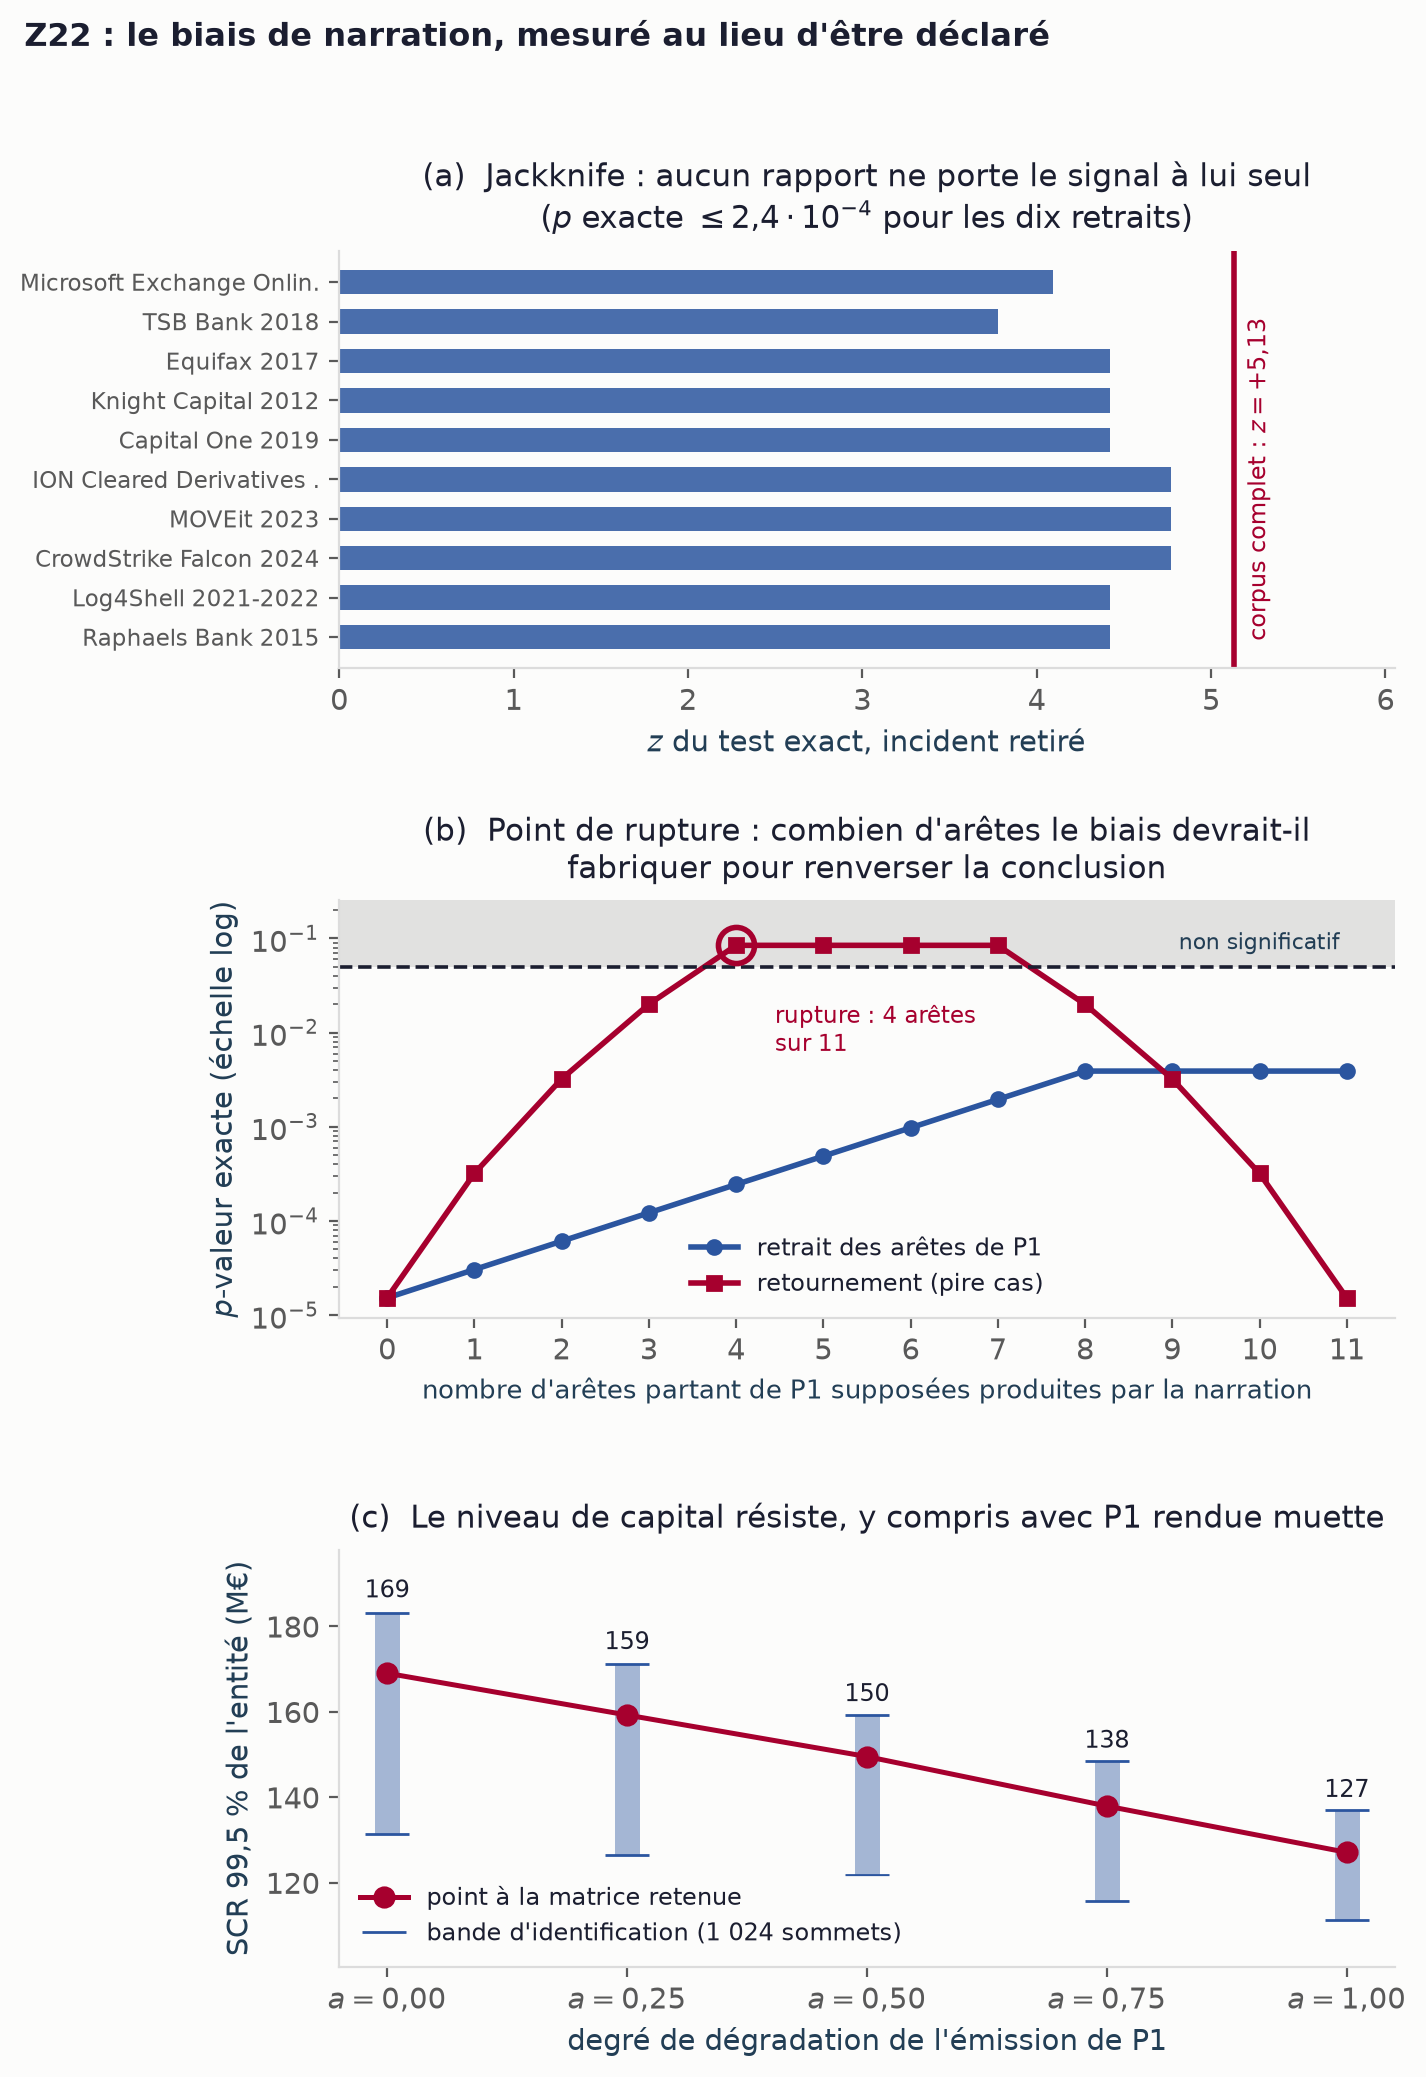
\includegraphics[width=0.99\textwidth]{Z22_biais_narration.png}
  \caption{Le biais de narration, mesuré au lieu d'être déclaré.
\textbf{(a)}~jackknife par incident : aucun rapport ne porte le signal à lui seul, les dix
retraits laissant $p \leq 2{,}4\cdot10^{-4}$. (b)~point de rupture, en $p$-valeur
exacte et non en $z$ : il faudrait quatre arêtes de $P_1$ retournées dans la pire configuration
pour perdre la significativité, et aucun nombre de retraits n'y suffit. La courbe de
retournement remonte au-delà de sept parce que retourner \emph{toutes} les arêtes n'efface pas
l'asymétrie, elle l'inverse. (c)~le niveau de capital résiste, y compris avec $P_1$
rendue muette, et la bande d'identification se resserre à mesure que l'émission de $P_1$
disparaît.}
  \label{fig:biais-narration}
\end{figure}
% SOURCES-SCRIPTS: 64

% =====================================================================
\section{La direction bayésienne : prior sceptique et crédibilité par paire}
\label{sec:ann-bayes}

% SOURCES-SCRIPTS: 56

Cette pièce accompagne le \S\ref{sec:bayes}.

Deux vérifications s'imposent, et elles vont dans des sens opposés. La première est rassurante :
sous un prior sceptique $\mathrm{Beta}(4,4)$, qui tire vers $\theta=1/2$ donc vers
l'absence de direction et qui est le plus défavorable à la thèse, la médiane ne se déplace que de
$0{,}8\,\%$. La conclusion vient donc des comptes documentés, non du prior. La seconde est une
mise en garde, et elle est décisive : par paire, seules deux des six paires documentées
ont un intervalle de crédibilité à $90\,\%$ qui exclut $\theta=1/2$. Avec une à trois chaînes
observées, l'espérance penche nettement mais la crédibilité ne suffit pas. Le test de signe de
la section~\ref{sec:postmortems} répondait à une \emph{autre} question, celle de la cohérence
d'ensemble des dix-sept transitions ; le posterieur juge chaque paire séparément et se montre
plus prudent. Les deux lectures sont justes, et c'est la plus conservatrice qui doit être
retenue.

\begin{figure}[htbp]
\centering
\figover{Z19_bayes_direction.png}
\caption{Reformulation bayésienne de la direction. (a)~posterieurs par paire : les paires
documentées s'écartent de $\theta=1/2$, celles sans donnée restent uniformes. (b)~le capital
devient une loi, plus informative que des bornes de pire cas. (c)~robustesse au prior : la
médiane bouge de $0{,}8\,\%$, même sous prior sceptique.}
% SOURCES-SCRIPTS: 56
\label{fig:bayes}
\end{figure}

% =====================================================================
\section{Le benchmark copule sur plusieurs graines et plusieurs niveaux}
\label{sec:ann-benchmark-graines}

Cette pièce accompagne le \S\ref{sec:benchmark}.

\textbf{Le $+0{,}1\,\%$ est une graine, et la coïncidence est plus fragile que le nombre ne le
laisse croire.} La reprise du protocole sur quatre graines et un échantillon assez grand pour
qu'un quantile à $99{,}95\,\%$ ait un sens donne, au même niveau
% SOURCES-SCRIPTS: 80
$99{,}5\,\%$, un écart moyen de $+4{,}8\,\%$ d'étendue $10$ points entre graines. Le
$+0{,}1\,\%$ publié n'est donc pas faux, il est \emph{un tirage} : la conclusion à retenir n'est
pas que la gaussienne retombe exactement sur la cascade, c'est que leur écart ne dépasse
pas son propre bruit. L'énoncé faible est le seul qui tienne, et il suffit à l'argument.

\textbf{Et la séparation en queue ne vaut que pour la Student.} Le même protocole, décliné sur
huit niveaux de quantile de $50$ à $99{,}95\,\%$, marque d'une étoile les seules cases où l'écart
dépasse l'étendue entre graines. Au-delà de $99\,\%$, seule la Student sort de son
bruit, à $+20{,}4$, $+29{,}8$ puis $+31{,}2\,\%$ ; ni la gaussienne ni l'indépendance n'y
parviennent, leurs étendues atteignant $13$ et $31$ points. La raison est structurelle : la
Student est la seule des trois à porter une dépendance de queue \emph{asymptotique}. Le préprint
doit donc être cité sur le protocole, jamais sur l'ordre du résultat en queue, qui
dépend de l'indice de queue de la sévérité et non de l'architecture du modèle.

% =====================================================================
\section{La précision de simulation des six postures}
\label{sec:ann-postures}

% SOURCES-SCRIPTS: 46 51

Cette pièce accompagne le \S\ref{sec:predictive-robuste}.

\textbf{Les deux extrémités de l'échelle sont exactes, tout le bruit est au milieu.} Le point est
le quantile d'un ajustement unique et le pire-cas celui d'un $\xi$ \emph{posé} : ni l'un ni
l'autre ne comporte de simulation. Ce sont les postures intermédiaires, celles qui intègrent
l'incertitude, qui en héritent un bruit propre. Une posture plus riche est donc, à ce titre
précis, moins reproductible.

\textbf{La posture la plus prudente est la moins précise.} À $\beta=99\,\%$ l'écart-type de
simulation vaut $24$~M\euro, environ le double de celui des deux niveaux inférieurs, et la raison
est structurelle : un percentile à $99\,\%$ de la loi bootstrap s'estime sur bien moins de
tirages utiles que sa médiane, dans une queue lourde. Cela ne disqualifie pas la posture, mais
cela interdit de la citer à trois chiffres significatifs. Sur quatre rééchantillonnages, un
écart-type est lui-même connu à $40\,\%$ près : le classement de $\beta=90\,\%$ et
$\beta=95\,\%$ n'est donc pas résolu ici et n'a pas à l'être, seul le saut vers $\beta=99\,\%$
est net.

\textbf{Une conséquence de rédaction.} Toute grandeur simulée de cette section est publiée avec son
bruit. La VaR prédictive vaut ainsi $648$~M\euro{} sur un ensemble bootstrap de $2\,000$ tirages et
$645$ sur un ensemble de $3\,000$, celui de la figure : même estimateur, et un écart de
$3$~M\euro{} inférieur à un écart-type de simulation. Les deux valeurs sont un seul nombre, et le
bruit publié dit la précision à laquelle le lire.

\begin{figure}[htbp]\centering
\figover{J2_var_predictive.png}
\caption{VaR prédictive. (a)~le paramètre $\xi$ est incertain. (b)~les queues
\emph{plug-in} et prédictive ne divergent que loin dans la queue. (c)~le capital se lit
en profil et en bande.}
% SOURCES-SCRIPTS: 46
\label{fig:predictive}
\end{figure}
    % Réconciliations, inventaire, sensibilités
% =====================================================================================
% ANNEXE AJOUTEE LE 12 AOUT 2026, a la demande de Caroline Hillairet, qui a salue
% l'initiative de pallier le manque de donnees par un recueil d'avis d'experts et demande de
% mettre la methode de Cooke et le questionnaire en annexe.
%
% LE SENS DE L'ANNEXE A CHANGE AVEC LA DECISION DE NE PAS LANCER L'ELICITATION. Elle ne
% presente donc pas un protocole A VENIR mais un protocole PREPARE ET NON EXECUTE, avec le
% chiffrage de la raison. C'est un actif devant un jury qui demanderait pourquoi un modele dont
% la direction n'est pas identifiable ne recourt pas au jugement d'expert : la reponse existe,
% elle est chiffree, et le materiel est pret.
%
% ATTENTION AU PIEGE DU HARNAIS, ET IL A ETE RENCONTRE ICI. Une declaration
% HARNAIS-HORS-SCRIPT posee AVANT la premiere \section couvre tout le fichier : la premiere
% version de cette annexe declarait ainsi ses onze nombres d'un coup, dont les huit qui sont
% parfaitement verifiables. La declaration est donc descendue dans la seule section qui la
% justifie, et les autres citent leurs scripts.
% =====================================================================================

\chapter{Le protocole d'élicitation, préparé et non exécuté}
\label{ch:elicitation}

% SOURCES-SCRIPTS: 31 34 59

La direction de la matrice de contagion n'est pas identifiable sur la donnée disponible
(chapitre~\ref{ch:identifiabilite}). Le recours au jugement d'expert formalisé est la réponse
classique à ce genre d'impasse, et un protocole complet a été construit pour cela. Il n'a pas
été exécuté, et cette annexe existe pour que ce choix soit lisible : le protocole y est décrit,
la raison de ne pas le lancer y est chiffrée, et ce que l'on perd y est dit.

\section{La méthode de Cooke, en quatre temps}

% HARNAIS-HORS-SCRIPT: les quantiles demandes a l'expert sont une propriete de CONCEPTION du
% questionnaire, non une grandeur calculee : aucun script ne les imprime et aucun ne le devrait.

Le \emph{modèle classique} de Cooke ne traite pas les experts comme interchangeables : il les
\emph{note}, sur des questions dont l'analyste connaît la réponse, puis pondère leurs avis par
cette note. Il se déroule en quatre temps.

\begin{enumerate}[itemsep=3pt,topsep=3pt]
\item \textbf{Élicitation en quantiles.} Chaque expert ne donne pas un point mais trois
      quantiles, à $5$, $50$ et $95\,\%$, ce qui rend son incertitude déclarée mesurable.
\item \textbf{Calibration.} Sur les \emph{questions-graines}, dont la réponse est connue de
      l'analyste et masquée à l'expert, on compare la fréquence empirique des réalisations dans
      les intervalles déclarés à la fréquence théorique. L'écart se lit comme une statistique
      d'information de Kullback-Leibler, et son niveau de signification devient le
      score de calibration.
\item \textbf{Information.} Un expert bien calibré mais qui déclare des intervalles très larges
      n'apporte rien. Le score d'information mesure la concentration de ses
      distributions relativement à une loi de référence.
\item \textbf{Poids et agrégation.} Le poids d'un expert est le produit des deux scores, et il
      est nul sous un seuil de calibration. L'avis agrégé est la combinaison linéaire
      pondérée des distributions individuelles.
\end{enumerate}

C'est le quatrième point qui fait la force et la fragilité de la méthode : un expert mal
calibré est écarté, ce qui protège des dires péremptoires, mais réduit d'autant la taille
effective du panel.

\section{Le protocole construit pour la matrice de contagion}

Le questionnaire préparé comporte deux parties. La partie d'étalonnage pose des
questions à réponse connue, tirées de sources publiques vérifiables, sur des grandeurs du même
domaine que les cibles. La partie cible interroge les liens dirigés entre piliers, un
par un, sous la forme d'une probabilité conditionnelle : sachant que le pilier source est
défaillant, quelle est la probabilité que le pilier cible le devienne.

Le dispositif complet demande seize questions par expert, dont dix questions-graines. Ce ratio
n'est pas un excès de prudence : c'est le minimum qui permette de distinguer un expert calibré
d'un expert chanceux, et le réduire viderait la méthode de ce qui la distingue d'une moyenne
d'opinions. Le protocole, le questionnaire et le gabarit de réponses sont versionnés dans le
dépôt du mémoire, et deux scripts implémentent l'agrégation, l'un sur réponses fictives pour
valider la chaîne de traitement, l'autre prêt à recevoir des réponses réelles.

\paragraph{Une dixième graine a été retirée, et le dire fait partie du protocole.} La première
version de l'étalonnage portait une question sur l'indice de queue de sévérité $\xi$, de valeur
vraie annoncée $0{,}90$. Deux défauts s'y cumulaient. D'abord $0{,}90$ n'est pas la calibration
mais la valeur \emph{posée} du scénario de pire cas, la calibration figée donnant
$\hat\xi = 0{,}5954$ : or dans la méthode de Cooke une graine fausse n'ajoute pas du bruit, elle
\emph{inverse} les poids, en pénalisant le répondant qui vise juste. Ensuite, et c'est ce qui
justifie le retrait plutôt que la correction, $\xi$ est une \emph{estimation} d'intervalle
$[0{,}30\,;0{,}83]$, plus large que la valeur elle-même : une graine doit être une grandeur
réalisée, pas un paramètre estimé. Les dix graines de l'instrument révisé sont toutes reproductibles par une
sortie de script versionnée, ce qui est la condition pour qu'une notation d'expert soit
opposable.

\vspace{2pt}
% SOURCES-SCRIPTS: 26 47 63

%--------------------------------------------------------------
\section{Le questionnaire, reproduit}
\label{sec:questionnaire-reproduit}
%--------------------------------------------------------------
% LES VALEURS VRAIES DES GRAINES NE SONT PAS PUBLIEES ICI, ET C'EST DELIBERE : les imprimer
% BRULERAIT l'instrument, un expert qui a lu le memoire ne pouvant plus etre note dessus. Le
% script 105 les calcule, leur applique quatre controles et les imprime dans sa sortie de
% travail ; si l'elicitation etait lancee apres publication, les graines se retirent du meme jeu
% de donnees par ce meme script. Ce qui est cite ci-dessous est donc le seul nombre que
% l'arbitrage de conception exige de montrer, la valeur du candidat ecarte.
% SOURCES-SCRIPTS: 105

Décrire un instrument ne suffit pas à établir qu'il existe. Il est donc reproduit ici dans la
forme sous laquelle il aurait été soumis, de façon qu'un lecteur puisse juger sur pièce ce que
la section précédente affirme, et le réutiliser si la décision était rouverte. Le formulaire
complet, avec sa consigne, son exemple traité, sa mention d'usage et de conservation et son
accord signé du répondant, est versionné à part dans le dépôt du mémoire ; la présente annexe en
reprend les deux tables et l'essentiel de la consigne.

\begin{attention}
\textbf{L'instrument reproduit ici est la version révisée, et il diffère de l'exemplaire de
travail.} Celui-ci portait une question d'étalonnage sur l'indice de queue de sévérité, retirée
pour les deux motifs exposés plus haut. Elle n'est pas corrigée mais \emph{remplacée}, et le
remplacement a lui-même été arbitré : un indice de Gini de la concentration avait d'abord été
retenu, puis écarté parce qu'il fait doublon avec la question qui compte les incidents portant la
moitié du volume, et parce qu'une valeur vraie de $0{,}97$ se devine sans rien connaître du
dossier. La graine retenue porte sur la durée de confinement, qui est une performance de
résilience et donc du même domaine que les cibles. \textbf{L'exemplaire de travail ne doit pas
être soumis en l'état.}
\end{attention}

\paragraph{La règle que s'impose l'instrument, et elle est vérifiée.} Une graine doit être une
\emph{grandeur réalisée}, reproductible par une sortie de script versionnée, et jamais un
paramètre estimé. Les dix graines retenues sont donc des comptages, des parts, des délais ou des
quantiles observés : aucune ne demande d'ajuster un modèle. Un script les calcule et leur applique
quatre contrôles, portant sur ce caractère réalisé, sur la non-dégénérescence de la valeur, sur le
respect des bornes naturelles, et sur le pouvoir de séparation entre experts. Une seule graine est
signalée comme potentiellement devinable, celle qui porte sur la part du piratage, et elle est
conservée avec son motif : sa valeur vraie est nettement au-dessus de la réponse spontanée, si
bien qu'elle sépare malgré son caractère extrême.

\paragraph{Aucune graine ne porte une grandeur de capital, et c'est délibéré.} Un praticien de la
résilience observe des incidents, des délais et des concentrations ; il n'observe pas un quantile
de charge annuelle. Noter un expert sur une telle grandeur mesurerait sa familiarité avec le
présent mémoire, non son jugement sur le risque.

\subsection*{Consigne remise à l'expert}

\begin{cle}
\textbf{Comment répondre.} Pour chaque quantité, donnez trois nombres : une valeur \emph{basse}
($5\,\%$), une valeur \emph{médiane} ($50\,\%$), une valeur \emph{haute} ($95\,\%$), telles que
vous estimez à $90\,\%$ de chances que la vraie valeur soit comprise entre votre $5\,\%$ et votre
$95\,\%$. Il n'y a pas de réponse attendue : donnez votre meilleure estimation \emph{et} votre
incertitude. Répondez même incertain, un intervalle large étant une réponse honnête et
parfaitement valable. Ne cherchez pas les vraies valeurs : l'objet est de mesurer votre jugement.
\end{cle}

\subsection*{Partie A, les dix questions d'étalonnage}

Des quantités observées dans les bases du mémoire, dont la valeur vraie est connue de l'analyste
et n'est pas affichée au répondant. Elles servent à pondérer les experts, non à les piéger. Les
trois colonnes de droite sont vides dans les deux tables qui suivent : c'est l'espace de réponse
du formulaire, non une donnée manquante.

{\small
\renewcommand{\arraystretch}{1.22}
\begin{longtable}{@{}l p{8.0cm} c c c@{}}
\toprule
& \textbf{Quantité, sur les incidents notifiés de la chronologie} & $\mathbf{5\,\%}$ &
$\mathbf{50\,\%}$ & $\mathbf{95\,\%}$ \\
\midrule
\endfirsthead
\toprule
& \textbf{Quantité (suite)} & $\mathbf{5\,\%}$ & $\mathbf{50\,\%}$ & $\mathbf{95\,\%}$ \\
\midrule
\endhead
G1 & Délai médian entre la survenance d'un incident et sa déclaration, en jours & & & \\
G2 & Part des incidents déclarés plus de quatre-vingt-dix jours après leur survenance,
     en \% & & & \\
G3 & Délai médian de déclaration d'un incident de type piratage, en jours & & & \\
G4 & Durée médiane entre le début et la fin d'exposition d'un incident, en jours & & & \\
G5 & Nombre médian d'enregistrements touchés par incident & & & \\
G6 & Nombre d'incidents qui portent à eux seuls la moitié du volume touché
     sur sept exercices & & & \\
G7 & Part des incidents dont l'exposition a duré plus de trente jours, en \% & & & \\
G8 & Part des incidents de type piratage parmi ceux dont le vecteur est renseigné,
     en \% & & & \\
G9 & Part des lignes de la chronologie qui sont des doublons de notification d'un même
     incident, en \% & & & \\
G10 & Rapport du quatre-vingt-dix-neuvième centile à la médiane des pertes cyber du
      secteur financier & & & \\
\bottomrule
\end{longtable}}

\vspace{2pt}
\noindent\textbf{Ce que chaque graine cherche à mesurer.} G1 à G3 portent sur le \emph{délai de
détection}, qui est le canal que la conformité déplace le plus directement. G4 et G7 portent sur
le \emph{confinement}. G5, G6 et G10 portent sur la \emph{concentration} de la perte, c'est-à-dire
sur l'intuition de queue lourde. G8 porte sur la structure des vecteurs et G9 sur la qualité de la
donnée déclarative, dont un praticien de la notification a une expérience directe.

\subsection*{Partie B, les six liens dirigés entre piliers}

Force du lien dirigé de $j$ vers $k$, entre $0$ et $1$ : $0$ signifie qu'une défaillance du
pilier $j$ n'entraîne jamais celle de $k$, $1$ qu'elle l'entraîne quasi certainement dans la
foulée. Les trois mêmes quantiles sont demandés.

\begin{attention}
\textbf{Le sens des lettres n'est pas une coquette\-rie de notation.} La matrice du modèle
s'écrit $W_{jk}$ avec $j$ la \emph{source} et $k$ la \emph{cible} : la ligne émet, la colonne
reçoit, et deux scripts vérifient cette convention avant tout calcul. Un formulaire qui
demanderait la force du lien \emph{de $k$ vers $j$} ferait donc saisir la matrice
\emph{transposée}. Or c'est précisément entre une matrice et sa transposée que le
chapitre~\ref{ch:identifiabilite} montre que la donnée ne tranche pas, et le
chapitre~\ref{chap:cascade} que le capital et la décision diffèrent. Une inversion de lettres
dans l'instrument produirait donc exactement l'erreur que tout le mémoire s'emploie à ne pas
commettre, et elle ne serait rattrapée par aucun contrôle numérique.
\end{attention}

{\small
\renewcommand{\arraystretch}{1.25}
\begin{longtable}{@{}l p{8.2cm} c c c@{}}
\toprule
& \textbf{Lien dirigé $j \rightarrow k$, $j$ émet} & $\mathbf{5\,\%}$ & $\mathbf{50\,\%}$ &
$\mathbf{95\,\%}$ \\
\midrule
\endfirsthead
\toprule
& \textbf{Lien dirigé (suite)} & $\mathbf{5\,\%}$ & $\mathbf{50\,\%}$ & $\mathbf{95\,\%}$ \\
\midrule
\endhead
B1 & P1 $\rightarrow$ P2 : une défaillance de gouvernance entraîne des incidents & & & \\
B2 & P2 $\rightarrow$ P1 : des incidents entraînent une défaillance de gouvernance & & & \\
B3 & P4 $\rightarrow$ P2 : une défaillance d'un tiers entraîne des incidents & & & \\
B4 & P1 $\rightarrow$ P4 : une défaillance de gouvernance entraîne une défaillance côté
     tiers & & & \\
B5 & P3 $\rightarrow$ P1 : une défaillance des tests de résilience entraîne une défaillance
     de gouvernance & & & \\
B6 & P5 $\rightarrow$ P2 : une défaillance du partage d'information entraîne des
     incidents & & & \\
\bottomrule
\end{longtable}}

\paragraph{Le couple B1 et B2 est l'objet même du mémoire.} Les deux questions portent sur le
\emph{même} couple de piliers, dans les deux sens. Une donnée de co-occurrence ne les distingue
pas ; un expert, lui, peut les séparer. C'est précisément la quantité que le
chapitre~\ref{ch:identifiabilite} montre non identifiable, et c'est la raison pour laquelle ce
questionnaire aurait eu une valeur que nulle autre source du dossier ne porte.

\paragraph{Ce qui est fait des réponses.} La partie~A mesure la calibration du répondant, c'est-à-dire
la justesse de ses intervalles, et son information, c'est-à-dire leur finesse ; ces deux
grandeurs fixent son poids dans l'agrégation. La partie~B, pondérée par ce poids et croisée avec
les réponses des autres experts, produirait chaque lien de la matrice sous forme d'\emph{intervalle}
et non de point. Le traitement est automatique et aucune donnée d'incident n'est requise, seulement
le jugement.

\section{Pourquoi il n'a pas été exécuté}

La raison est arithmétique, et elle porte sur la \emph{taille effective} du panel.

\paragraph{Un panel de deux experts n'a aucun pouvoir de calibration.} Avec le calendrier du
mémoire et un taux de réponse réaliste sur un questionnaire de seize questions quantitatives, le
nombre de réponses exploitables, c'est-à-dire complètes et passant le seuil de calibration,
serait de l'ordre de une à deux. Or à deux experts la pondération de Cooke dégénère : soit un
seul survit au seuil et l'on obtient un avis unique déguisé en agrégation, soit les deux
survivent et le poids relatif est estimé sur dix graines, ce qui ne le distingue pas d'une
moyenne simple. Dans les deux cas la méthode ne fait plus ce pour quoi elle est choisie.

\paragraph{Et une élicitation faible ne serait pas neutre, elle serait trompeuse.} C'est
l'argument décisif, et il est chiffré. Le chapitre~\ref{chap:partielle} mesure l'effet d'un
panel biaisé sur le capital : il déplace le \textsc{scr} de $777$~M\euro{} sans
qu'aucun signal ne l'indique au lecteur, là où l'approche par bornes reste \emph{invariante} à
ce biais. Un jugement d'expert faiblement calibré introduirait donc dans le résultat une
incertitude \emph{non déclarable}, alors que la non-identifiabilité, elle, se déclare et se
borne. En termes de qualité de la conclusion, l'échange serait défavorable : on remplacerait
une ignorance mesurée par une erreur invisible.
% SOURCES-SCRIPTS: 31

\paragraph{Une asymétrie à assumer, car un relecteur la trouvera.} Cet argument condamne le
jugement d'expert non vérifiable, or ce mémoire \emph{utilise} du jugement d'expert ailleurs :
la direction de la contagion s'appuie sur un corpus de dix rapports codés, et par un seul codeur
à ce jour. Refuser l'élicitation au nom du biais d'expert tout en s'appuyant sur un codage
d'expert demande donc une justification, et non un silence.

Elle tient en trois différences, et c'est leur cumul qui compte. Le codage est
\emph{auditable} : le protocole est écrit, les dix récits sont publics, et n'importe qui peut
recoder le corpus et confronter ses réponses aux nôtres, ce qu'une élicitation quantitative en
séance ne permet pas. Son biais principal est mesuré plutôt que redouté : le biais de
narration fait l'objet d'un test contre une loi nulle exacte, dont le résultat est publié
\emph{et négatif} (\S\ref{sec:biais-narration}). Et son produit est un ordre partiel,
un objet qualitatif que la suite du raisonnement borne, là où une élicitation produirait des
coefficients numériques entrant directement dans le capital. Un dire d'expert qui alimente une
borne et un dire d'expert qui alimente un nombre n'engagent pas le même risque.

Reste que la comparaison n'est pas entièrement favorable : le codage demeure à juge
unique, et cela se lit comme une limite déclarée et non comme une étape en attente. Ce
qui la distingue du défaut reproché à l'élicitation est qu'elle est \emph{bornée} : la
dégradation complète de la source contestée coûte moins que l'ignorance directionnelle déjà
publiée (\S\ref{sec:biais-narration}), là où un panel faiblement calibré introduirait une
incertitude non déclarable. Un second codage en aveugle renforcerait l'énoncé, et le dispositif
reste préparé à cette fin.

\section{Ce qui le remplace}

Trois dispositifs, tous en place et tous sans prior d'expert.

\begin{description}[itemsep=3pt,topsep=3pt]
\item[Le corpus documentaire.] Dix rapports post-mortem officiels sont codés selon un protocole
      écrit, et le sens des transitions y est testé contre une loi nulle exacte de permutation :
      $z = +5{,}12$ sur le corpus étendu. La direction n'est donc pas seulement posée, elle est
      \emph{corroborée} par une source indépendante du classeur qualitatif.
\item[L'échelle de repli sur la direction.] Plutôt que de connaître la direction, on peut
      supposer qu'elle est de rang faible. Le premier cran de cette échelle capte $74{,}1\,\%$
      de la variance de la direction posée et resserre le capital dans
      $[7\,761\,;\,8\,316]$~M\euro, soit une largeur de $555$~M\euro{} contre $1\,839$ sous
      ignorance totale. C'est une hypothèse structurelle, déclarée comme telle, et bien plus
      modeste qu'un dire d'expert.
\item[Les ancrages réglementaires.] Les niveaux d'exigence des textes et les publications des
      autorités fournissent des repères externes sur les états de conformité, sans passer par un
      panel.
\end{description}

% SOURCES-SCRIPTS: 30 34 59

\section{La relecture de praticien et son résultat}
\label{sec:relecture-praticien}

\paragraph{Pourquoi ce dispositif est nécessaire, et il l'est pour une raison qui n'a rien de
conjoncturel.} La direction de $W$ n'est pas identifiable sur les données disponibles,
et le chapitre~\ref{ch:identifiabilite} le démontre plutôt que de le déplorer : les statistiques
que les sources permettent de construire sont aveugles à la partie antisymétrique, donc une
matrice et sa transposée y sont indiscernables. Il en résulte que $W$ n'est pas calibrée au sens où le sont la fréquence et
la sévérité. Sa structure est \emph{déduite} d'un corpus de rapports post-mortem, source qui
porte son propre confondant, le biais de narration d'une enquête officielle, borné au
\S\ref{sec:biais-narration} mais non levé.

Sur une structure ainsi posée, il ne reste qu'un seul contrôle externe possible : le
jugement de praticiens qui ont vu des défaillances réelles, et qui n'ont lu ni le corpus ni le
mémoire. Ce dispositif est donc nécessaire et non facultatif. Mais il faut voir ce
qu'il peut et ce qu'il ne peut pas : un praticien peut corroborer ou contredire une
structure, il ne peut pas la calibrer, faute de quoi on retomberait sur l'élicitation
que ce chapitre vient d'écarter, avec son déplacement de capital non déclarable. C'est
exactement la différence entre une relecture et une élicitation, et elle commande la forme de
l'instrument.

Le dispositif est donc de nature différente des trois précédents : non pas recueillir des
probabilités, mais soumettre à des praticiens du secteur les affirmations \emph{qualitatives}
sur lesquelles le modèle repose, en leur demandant de les contredire. L'instrument est
un questionnaire de sept phrases, sans lecture préalable du mémoire, dont deux portent
explicitement sur l'ordre P1 vers P2. Le choix de demander des désaccords plutôt que des
accords est délibéré : un accord ne discrimine rien, alors qu'un désaccord argumenté désigne
l'endroit exact où le modèle s'écarte de ce que le terrain observe.

\paragraph{La première réponse ne contredit rien.} Une consultante de Nexialog, exerçant en
gestion des risques et du contrôle depuis une dizaine d'années, n'a contredit aucune
des sept phrases : deux accords pleins, cinq accords assortis d'une nuance. Un instrument
construit pour recueillir des désaccords et qui n'en recueille aucun renseigne d'abord sur
lui-même, et cette information vaut d'être écrite plutôt que passée sous silence.

\paragraph{Ce que la réponse corrobore, et ce n'est pas la direction.} Deux affirmations
reçoivent un accord franc et argumenté, et toutes deux portent sur la \emph{faisabilité} des
recommandations plutôt que sur la structure du modèle. Sur les trois indicateurs pilotables,
la répondante les juge cohérents et produisibles, et suggère de les compléter par une fréquence
d'occurrence. Sur le registre d'incidents mieux spécifié, qui est le prolongement le plus utile
identifié par ce mémoire, elle va plus loin que l'accord : elle décrit un usage professionnel
établi, un tableau de bord des incidents par prestataire servant, dans une analyse de risque
conduite au titre de DORA, à évaluer la fréquence du risque de défaillance système et le taux
d'indisponibilité sur douze mois. La recommandation la moins mathématique du mémoire est donc
aussi celle que le terrain confirme le plus directement.

\paragraph{Une qualification substantielle, qu'il faut déclarer sans la traiter.} La nuance la
plus utile porte sur l'arc de la gouvernance vers la gestion des prestataires tiers. La
répondante distingue l'occurrence et la maîtrise : une gouvernance solide ou
fragile ne change pas, selon elle, le fait qu'un prestataire critique tombe, mais elle change
la capacité de l'entité à en limiter les conséquences. Traduite dans les termes du modèle,
cette distinction déplacerait cet arc de la matrice de propagation vers le canal de détection,
ce qui n'est pas la même chose et ne donne pas le même chiffre. La réserve est donc
déclarée et non traitée : la traiter reviendrait à recalibrer, ce que le gel interdit,
et une réponse unique ne justifie pas de rouvrir la calibration.

\paragraph{Et un argument d'antériorité, le seul de la réponse qui soutienne vraiment un
ordre.} Sur la phrase qui fait de la gestion des incidents un puits, la répondante avance un
argument temporel plutôt qu'une intuition : les tests sont conduits en amont de la mise en
service, donc un incident postérieur ne peut pas dégrader les tests. C'est de la précédence, et
c'est précisément ce que le corpus documentaire code. Elle ajoute une critique de la définition
du pilier lui-même, en séparant l'incident de sa gestion, deux objets que la nomenclature
réglementaire réunit.

\paragraph{Ce que l'instrument devient.} Deux défauts du questionnaire ont été identifiés par
cette première réponse, tous deux dans les phrases et non chez la répondante. La phrase sur la
gouvernance source pure \emph{empaquetait} deux affirmations, et la répondante a nuancé la
première sans se prononcer sur la seconde, qui est celle qui compte. Et la phrase opposant la
contagion à la cause commune ne discriminait pas ce qu'elle prétendait discriminer, pour la
raison exposée au chapitre~\ref{ch:identifiabilite}. Trois questions à choix forcé ont été
ajoutées,
qui séparent les deux affirmations empaquetées, demandent au répondant de choisir entre
contagion et cause commune, et font trancher la distinction occurrence contre maîtrise. La
modalité \emph{je ne peux pas trancher} y est offerte explicitement, et c'est la plus
intéressante : un praticien qui la choisit corrobore la frontière d'identifiabilité sur le
terrain, ce qui vaut davantage qu'un accord sur la matrice.

\paragraph{La seconde réponse contredit deux phrases, et c'est ce que l'instrument cherchait.}
Un consultant de Nexialog, expert de la résilience et de la continuité d'activité dans les
services financiers depuis sept ans, a répondu à la même version du questionnaire, sans les
questions à choix forcé ajoutées depuis. Il ne se prononce pas sur la première phrase tout en la
commentant, donne quatre accords assortis d'une nuance, et exprime deux désaccords argumentés,
sur les deux phrases que le questionnaire désignait comme les plus importantes.

\paragraph{La cause commune, avancée sans y être invité.} Sur la phrase qui oppose la contagion à
la cause extérieure commune, il reconnaît des chaînes de causalité, une gouvernance peu
structurée conduisant à des tests insuffisants puis à des incidents, mais ajoute que plusieurs
domaines peuvent céder ensemble parce qu'ils partagent une cause : un manque de ressources, une
transformation mal pilotée, une architecture vieillissante. Il conclut qu'il parlerait de
dépendances entre domaines plutôt que de causalité systématique. Là où la première réponse
illustrait la frontière d'identifiabilité sans la nommer, celle-ci la formule : c'est la
corroboration la plus nette que le dispositif ait produite, et elle porte sur la frontière, non
sur la matrice.

\paragraph{Deux désaccords sur le sens des arcs, déclarés.} Il conteste que la gouvernance soit une
source pure : un incident significatif peut conduire à changer les responsabilités, à renforcer
les comités de suivi ou à augmenter les budgets, si bien que la gouvernance est aussi une
conséquence des défaillances. Il conteste de même que la gestion des incidents soit un puits : un
incident mal géré révèle des tests insuffisants et conduit à les renforcer, un incident impliquant
un prestataire fait revoir les contrats et la surveillance, et une escalade défaillante dégrade la
circulation de l'information. Deux lectures de ces exemples doivent être tenues ensemble. La
plupart décrivent une rétroaction corrective, l'incident conduisant à renforcer un domaine :
elle relève de l'évolution des états de conformité modélisée au chapitre~\ref{chap:multietats},
non de la propagation d'une perte que porte la matrice. Un seul décrit une dégradation en retour,
de la gestion des incidents vers le partage d'information, sens qu'aucun rapport du corpus ne
code. Ce désaccord ne déplace pas le capital publié : l'ensemble admissible du
chapitre~\ref{chap:partielle} ne fixe aucune direction et contient aussi bien les matrices à
dépendance réciproque que celles où l'arc est inversé. Il affaiblit en revanche la structure que
le corpus suggère, déjà déclarée corroborée et non calibrée, et il est enregistré comme tel.

\paragraph{La faisabilité, sous conditions.} Il juge les trois indicateurs pertinents et
actionnables mais insuffisants à eux seuls, et y ajouterait les incidents récurrents, les
vulnérabilités critiques non corrigées, les résultats des tests et la disponibilité des services
critiques. Il juge le registre d'incidents réaliste, et la distinction entre date de survenue et
date de déclaration particulièrement utile, sous réserve de règles de qualification précises :
le classement d'un incident par domaine peut être subjectif, et reconnaître une cause commune à
plusieurs victimes suppose de disposer de l'information qui l'établit. Sur le prestataire
partagé, il confirme le choc simultané en rappelant que le niveau de dépendance résulte lui-même
de choix de gouvernance.

\paragraph{Ce qui manque selon lui.} La gestion des changements et celle des vulnérabilités,
qu'il désigne comme des déclencheurs fréquents d'une chaîne traversant plusieurs domaines sans
qu'aucun ait été défaillant au départ. Le modèle fait naître un incident sur un pilier ; un
déclencheur transversal de ce type n'y a pas de place propre, et c'est une limite de périmètre à
inscrire parmi les prolongements.

\paragraph{Statut.} Deux réponses ne font pas un panel. Cette relecture n'entre donc dans aucune
table de robustesse et ne modifie aucun niveau publié. Elle est citée pour ce qu'elle est, une
relecture de praticiens engagée et partiellement rendue, et les répondants ne sont pas nommés.

\section{Le coût de la décision et sa réversibilité}

Il faut nommer le coût. L'élicitation avait une fonction précise et une seule :
\textbf{départager P1 et P4} en tête du classement des piliers sources. Sans elle, les deux
restent pratiquement à égalité sur l'ensemble admissible, P1 arrivant premier dans
$43{,}6\,\%$ des configurations et P4 dans $37{,}7\,\%$, pour un écart de regret maximal de
$1{,}5\,\%$ (\S\ref{sec:res-prio}). Le mémoire conclut donc que P1 et P4 devancent nettement les
trois autres piliers, et il s'arrête là où la donnée s'arrête, au lieu de trancher entre eux par
un avis.
% SOURCES-SCRIPTS: 30 31

\begin{cle}
\textbf{Une décision, pas un renoncement.} Le protocole est écrit, le questionnaire est prêt, le
gabarit de réponses et la chaîne d'agrégation sont testés. Ce qui manque n'est pas le
dispositif mais un panel de taille suffisante pour que la pondération de Cooke ait un sens.
La décision est donc \emph{réversible sans coût de développement} : si un accès à un panel
d'une dizaine de répondants devient possible, l'élicitation reprend là où elle a été laissée,
et son apport attendu est connu d'avance, à savoir le départage de P1 et P4 et un resserrement
de la bande d'identification. C'est le seul point du mémoire où une donnée supplémentaire
changerait une conclusion plutôt qu'un niveau.
\end{cle}
    % Protocole de Cooke, préparé et non exécuté
\chapter{Table des notations}

% MIGRÉ depuis memoire/main.tex (plages 3230-3259).
% RELECTURE FAITE (août 2026) : la table héritée ne portait AUCUN symbole du
% modèle de cascade (W, S, A, TRANS, ROOT, g, s_j, e_j, R_0, t, kappa), alors
% que c'est le modèle central. Elle est réécrite et organisée en cinq blocs.
\label{not:ann:notations}

\noindent Les symboles sont regroupés par brique du modèle, dans l'ordre où le mémoire les
introduit. La colonne de droite renvoie au chapitre qui les définit.

\renewcommand{\arraystretch}{1.22}
\begin{center}\small
\begin{tabular}{>{\raggedright}p{3.3cm} >{\raggedright\arraybackslash}p{10.2cm} c}
\toprule
\rowcolor{lightblue}
\textbf{Symbole} & \textbf{Signification} & \textbf{Ch.} \\
\midrule
\multicolumn{3}{@{}l}{\textit{\textcolor{navy}{Piliers et cascade dirigée}}} \\
$P_1,\dots,P_5$ & Les cinq piliers DORA : gouvernance, gestion des incidents, tests de résilience, prestataires tiers, partage d'informations & \ref{chap:cascade} \\
$\mathrm{TRANS}$ & Matrice d'influence brute du classeur qualitatif, asymétrique, non normalisée & \ref{chap:cascade} \\
$\mathrm{ROOT}$ & Propension de chaque pilier à \emph{amorcer} une chaîne & \ref{chap:cascade} \\
$s_j$ & Somme de la ligne $j$ de $\mathrm{TRANS}$ ; $s_{\max}=\max_j s_j$ & \ref{chap:cascade} \\
$g$ & Gain de propagation, part de contagion du pilier le plus exposé & \ref{chap:cascade} \\
$W$ & Matrice de contagion normalisée à la Leontief, $W=g\,\mathrm{TRANS}/s_{\max}$ & \ref{chap:cascade} \\
$e_j$ & Propension à propager depuis $j$, $e_j=g\,s_j/s_{\max}$ & \ref{chap:cascade} \\
$\rho(W)$ & Rayon spectral de $W$ ; $\rho(W)\le g<1$ garantit la stabilité & \ref{chap:cascade} \\
$(I-W)^{-1}$ & Inverse de Leontief, descendance espérée avec multiplicité & \ref{chap:cascade} \\
$M,\ R_0$ & Matrice de génération suivante et son rayon spectral (extinction si $R_0<1$) & \ref{chap:cascade} \\
$S_a$ & Ensemble des piliers atteints depuis l'amorce $a$ & \ref{chap:cascade} \\
$K_j,\ u_j$ & Seuil sur la latente ; seuil de matérialité observable (art.~18) & \ref{chap:cascade} \\
\midrule
\multicolumn{3}{@{}l}{\textit{\textcolor{navy}{Identifiabilité et identification partielle}}} \\
$S,\ A$ & Parties symétrique et antisymétrique de $W$ : co-occurrence (identifiée) et direction (non identifiée) & \ref{ch:identifiabilite} \\
$J_{jk}$ & Courant de probabilité $\pi_jP_{jk}-\pi_kP_{kj}$ ; nul ssi réversibilité & \ref{ch:identifiabilite} \\
$\pi,\ \tilde P$ & Loi stationnaire ; noyau adjoint (chaîne renversée dans le temps) & \ref{ch:identifiabilite} \\
$\mathcal{E}(f,f)$ & Forme de Dirichlet, variation quadratique de la martingale ; ne dépend que de $S$ & \ref{ch:identifiabilite} \\
$\sigma$ & Production d'entropie ; nulle ssi la chaîne est réversible & \ref{ch:identifiabilite} \\
$T(M),\ z$ & Statistique d'asymétrie et son écart réduit au placebo par permutation & \ref{ch:identifiabilite} \\
$t$ & Degré d'ignorance directionnelle, $|A_{jk}|\le t\,S_{jk}$ ; $t=1$ = ignorance totale & \ref{chap:partielle} \\
$\mathcal{W}(t)$ & Ensemble admissible des matrices compatibles avec la donnée & \ref{chap:partielle} \\
$u_{ij}$ & Excès de propagation propre à la source, $\operatorname{logit}p_{ij}=\operatorname{logit}p_j+u_{ij}$ & \ref{chap:partielle} \\
$L(\mathcal{V}),\ V(\mathcal{I})$ & Largeur de bande de capital ; valeur d'une information & \ref{ch:livrable} \\
\midrule
\multicolumn{3}{@{}l}{\textit{\textcolor{navy}{Socle : fréquence et sévérité}}} \\
$\xi,\ \sigma_{\text{GPD}},\ u$ & Indice de queue, échelle et seuil POT de la GPD de sévérité & \ref{chap:socle} \\
$\zeta_u=p_u$ & Probabilité de dépassement du seuil, $\Prob(X>u)$ & \ref{chap:socle} \\
$N_u$ & Nombre d'excès au-delà de $u$ & \ref{chap:socle} \\
$\lambda_{ref}$ & Fréquence de référence PRC ($341$/an) : \emph{clé de répartition} par vecteur, n'alimente pas le moteur & \ref{chap:donnees} \\
$\lambda$ & Fréquence d'entrée du moteur, incidents \textsc{tic} matériels ($21{,}6$/an au secteur) & \ref{chap:donnees} \\
$\varphi,\ a$ & Facteur de surdispersion ; charge systémique commune du mélange lognormal & \ref{chap:socle} \\
$r,\ p$ & Paramètres de la loi binomiale négative de fréquence & \ref{chap:socle} \\
$b$ & Élasticité de la sévérité à la taille de la firme & \ref{chap:donnees} \\
\midrule
\multicolumn{3}{@{}l}{\textit{\textcolor{navy}{Conformité multi-états}}} \\
$C^\star_j,\ \Theta$ & Capacité de conformité latente du pilier $j$ ; facteur systémique commun & \ref{chap:multietats} \\
$\gamma$ & Charge systémique de la latente de conformité ($0{,}68$) & \ref{chap:multietats} \\
$K_{\text{bas}},K_{\text{haut}}$ & Seuils ordonnés découpant les états NC / PC / C & \ref{chap:multietats} \\
$Q$ & Générateur de la chaîne de Markov de mise en conformité (séjours de type phase) & \ref{chap:multietats} \\
$S_0,S_1,S_2$ & Scénarios conforme / partiel / non conforme (multiplicateurs de fréquence) & \ref{chap:socle} \\
\midrule
\multicolumn{3}{@{}l}{\textit{\textcolor{navy}{Capital, allocation et décision}}} \\
$\VaR_\alpha,\ \TVaR_\alpha$ & Value-at-Risk et Tail-VaR au niveau $\alpha=99{,}5\,\%$ & \ref{chap:socle} \\
$\Delta_{DORA}$ & Surcoût de capital imputable à la non-conformité & \ref{chap:resultats} \\
$AC_k,\ \phi_j$ & Contribution d'Euler ; valeur de Shapley du pilier $j$ & \ref{chap:resultats} \\
$\mathrm{CoC}$ & Taux de coût du capital de la marge de risque ($6\,\%$, révisé à $4{,}75\,\%$) & \ref{chap:resultats} \\
$L,\ L^\star$ & Portée d'un traité en excès de perte annuel ; portée optimale & \ref{chap:resultats} \\
$\kappa$ & Coefficient d'inefficacité du transfert (capacité, base, contrepartie) & \ref{chap:resultats} \\
$\theta$ & Paramètre de la copule de Gumbel, \emph{utilisée comme axe de comparaison} et non comme modèle & \ref{ch:robustesse} \\
\bottomrule
\end{tabular}
\end{center}

\clearpage

% =====================================================================
                % Table des notations

\bibliographystyle{plainnat-fr}
{\NoAutoSpacing\bibliography{references}}

\end{document}

% ---------------------------------------------------------------------
% NOTE SUR LE CHAPITRE DU CADRE REGLEMENTAIRE, ET C'EST UN CHOIX ASSUME.
% Le plan de restructuration prevoyait d'en degager deux pages par relecture
% resserree, avec une clause explicite : « si la relecture ne degage pas ce gain
% sans perte, le chapitre reste inchange ». Le chapitre ne porte aucune decoupe en
% sections, donc le gain n'etait accessible que par reecriture de prose
% reglementaire, a dix-neuf jours du depot et sur un texte qui cite des articles.
% La clause joue : le chapitre est repris tel quel. C'est deux pages de moins que
% la cible, et il vaut mieux le dire que de le masquer.
